%% ----------------------------------------------------------------
%% Thesis.tex -- MAIN FILE (the one that you compile with LaTeX)
%% ---------------------------------------------------------------- 

% Set up the document
\documentclass[a4paper, 12pt, oneside]{uet_thesis}  % Use the "Thesis" style, based on the ECS Thesis style by Steve Gunn
\graphicspath{{Figures/}}  % Location of the graphics files (set up for graphics to be in PDF format)

% Include any extra LaTeX packages required
\usepackage[square, numbers, comma, sort&compress]{natbib}  % Use the "Natbib" style for the references in the Bibliography

\usepackage{verbatim}  % Needed for the "comment" environment to make LaTeX comments

%\usepackage{vector}  % Allows "\bvec{}" and "\buvec{}" for "blackboard" style bold vectors in maths

\usepackage{url}
\usepackage{natbib}


% for horizontal table 
\usepackage{booktabs}



\usepackage{array}
\usepackage[export]{adjustbox}
\usepackage{amsmath}
\hypersetup{urlcolor=blue, colorlinks=true}  % Colours hyperlinks in blue, but this can be distracting if there are many links.

% remove the unnecessary spacing before and after the headings/subheadings
\usepackage[compact]{titlesec}
\titlespacing{\section}{0pt}{*0}{*0}
\titlespacing{\subsection}{0pt}{*0}{*0}
\titlespacing{\subsubsection}{0pt}{*0}{*0}

\setlength{\parskip}{6pt}
%\setlength{\parsep}{0pt}
%\setlength{\headsep}{0pt}
%\setlength{\topskip}{0pt}

%% ----------------------------------------------------------------
\begin{document}
\frontmatter	  % Begin Roman style (i, ii, iii, iv...) page numbering

% Set up the Title Page
\title  {Digital Board Marker (Storage Efficient System for Class Lectures)}
\session {2016 -- 2020}
\advisor {Samyan Qayyum Wahla}
\authors {  % please enter the students names and registration numbers
Muhammad Haris Khan \quad 2016-CS-105 \\Hamza Farooq  \quad 2016-CS-122 \\Ayesha Atif\quad 2016-CS-152 \\Komal Shehzadi \quad 2016-CS-178 }

\addresses  {\deptname \\ \univname}  % Do not change this here, instead these must be set in the "Thesis.cls" file, please look through it instead
\date       {\today}
\subject    {}
\keywords   {}

\maketitle
%% ----------------------------------------------------------------

\setstretch{1.3}  % It is better to have smaller font and larger line spacing than the other way round

% Define the page headers using the FancyHdr package and set up for one-sided printing
\fancyhead{}  % Clears all page headers and footers
\rhead{\thepage}  % Sets the right side header to show the page number
\lhead{}  % Clears the left side page header

\pagestyle{fancy}  % Finally, use the "fancy" page style to implement the FancyHdr headers


%% Select only one of the certification pages  
%\CertificationMSc{}
%\CertificationBSc{}
\clearpage  % Certification ended, now start a new page


%% ----------------------------------------------------------------
% Declaration Page required for the Thesis, your institution may give you a different text to place here
\Declaration{
%\addtocontents{toc}{\vspace{1em}}  % Add a gap in the Contents, for aesthetics

We declare that the work contained in this thesis is our own, except where explicitly stated otherwise. In addition this work has not been submitted to obtain another degree or professional qualification.

\bigskip

Signed:~~ \rule[0em]{10em}{1.0pt} \\ % This prints a line for the signature 
Date:~~~~ \rule[0em]{10em}{1.0pt}  % This prints a line to write the date
}
\clearpage     % Declaration ended, now start a new page

%% ----------------------------------------------------------------

\setstretch{1.3}  % Reset the line-spacing to 1.3 for body text (if it has changed)

% The Acknowledgements page, for thanking everyone
\acknowledgements{
%\addtocontents{toc}{\vspace{1em}}  % Add a gap in the Contents, for aesthetics

First of all, we wish to thank Almighty Allah for giving us strength in fulfilling this work. It gives us great pleasure to express our deep sense of gratitude and respect to our supervisor, Sir Samyan Qayyum Wahla, for boasting our confidence and a sense of excitement and inspiring us in our work through his guidance. Our sincere thanks to him for his valuable suggestions and efforts. It is with great pride and pleasure that we submit this dissertation as his students. Lastly we would like to thank our parents for their unconditional, love, affection, kind cooperation and encouragement.

}
\clearpage  % End of the Acknowledgements

%% ----------------------------------------------------------------
% End of the pre-able, contents and lists of things
% Begin the Dedication page
\setstretch{1.3}  % Return the line spacing back to 1.3
\pagestyle{empty}  % Page style needs to be empty for this page
\dedicatory{To out parents and respected members}


%% ----------------------------------------------------------------
\pagestyle{fancy}  %The page style headers have been "empty" all this time, now use the "fancy" headers as defined before to bring them back

%% ----------------------------------------------------------------
\lhead{\emph{Contents}}  % Set the left side page header to "Contents"
\tableofcontents  % Write out the Table of Contents

%% ----------------------------------------------------------------
\lhead{\emph{List of Figures}}  % Set the left side page header to "List if Figures"
\listoffigures  % Write out the List of Figures

%% ----------------------------------------------------------------
\lhead{\emph{List of Tables}}  % Set the left side page header to "List of Tables"
\listoftables  % Write out the List of Tables

%% ----------------------------------------------------------------
\setstretch{1.5}  % Set the line spacing to 1.5, this makes the following tables easier to read
\clearpage  % Start a new page
\lhead{\emph{Abbreviations}}  % Set the left side page header to "Abbreviations"
\listofsymbols{ll}  % Include a list of Abbreviations (a table of two columns)
{
% \textbf{Acronym} & \textbf{W}hat (it) \textbf{S}tands \textbf{F}or \\
\textbf{LAH} & \textbf{L}ist \textbf{A}bbreviations \textbf{H}ere \\
}

%% ----------------------------------------------------------------
% The Abstract Page
\addtotoc{Abstract}  % Add the "Abstract" page entry to the Contents
\abstract{
%\addtocontents{toc}{\vspace{1em}}  % Add a gap in the Contents, for aesthetics

In a new educational concept, the Lecture Recording system is one of the devices that are widely used to provide educational material to students. Lecture recording plays an important role in online learning and distance education. Most of they are recorded by a cameraman or a static camera. But high resolution recorded video require lot of storage space and also the internet bandwidth. In this work, a storage and bandwidth efficient lecture recording system is proposed to minimize the storage and bandwidth issues. This system is 100 times more efficient that the previously developed lecture recording system. This system is also small in size and portable. This lecture recording system allows students to re-experience the lecture session at anytime and anywhere by downloading it with the minimum bandwidth available or viewing it through the portal. It is made public to promote research and further development in this system. The proposed system is combination of hardware module and software modules. Its first step is position detection at each point of board marker through stereo vision cameras to generate a file that will later be easily played offline as well as online on the web portal. \ldots

}
\clearpage  % Abstract ended, start a new page

%% ----------------------------------------------------------------
\mainmatter	  % Begin normal, numeric (1,2,3...) page numbering
\pagestyle{fancy}  % Return the page headers back to the "fancy" style
\onehalfspacing
% Include the chapters of the thesis, as separate files
% Just uncomment the lines as you write the chapters

% Chapter 1

\chapter{Introduction} % Write in your own chapter title
\label{Chapter1}
\lhead{Chapter 1. \emph{Introduction}} % Write in your own chapter title to set the page header
\section{Overview of the Project}
Digital board marker is a size efficient, bandwidth saving lecture recording system. It can record lecture, providing automated google search of handwritten words. Provides on the spot wiki. Lecture text notes can be generated automatically. Lecture can be named and divided into topics and subtopics automatically. According to a survey, 94\% students go for online help of recently attended lectures because they can't fully grab the concepts. Recorded lectures as video format require so much internet bandwidth to play. In most cases, large sized videos are difficult to handle or download. Because students mostly don't have huge amount of extra space available especially for the CSE students, as they already use bulky software and also students don't have large amount of bandwidth of internet available.
\bigskip

\section{Background}
Mostly systems for online video lecture that exist now a days work on the principle of simple video recording and a website for that organization. The systems like edx, coursera, MIT Open Courseware simple records mp4(or any other format) video and then upload it on their website in a particular section related to particular course. Some of them allow to download the videos. These mp4 videos of 1 hour can take upto 900mb to 1gb of storage space and internet data.\\
Now DBM came up with the solution of this large storage issue and more internet usage. Instead of recording video it stores position of a pen from which teacher is writing on the white-board. Since position of pen/marker is stored in a text/json file which will reduce the size upto 100 times. 

%The main aim of digital board marker is to provide ease to the students of all the educational institutes. Mostly lecture systems that already exist, of different universities, provide lectures online on youtube but the problem is they need great internet bandwidth and lot of memory to download and watch the lectures which is difficult for students especially in Pakistan. So that we provide bandwidth and storage efficient lecture system.\\
%Universities are places of knowledge production, and the economy and society are the users of this knowledge. So universities can provide ease to student with this system.
\bigskip

\section{Motivation}
The motivation and purpose to do this project is to minimize the use of resources that are used in lecture systems now a days working in all over the world i.e. video lecture recording and streaming through internet. 

\begin{itemize}

\item The first motivation is to deal with the large amount of storage that normally video lectures take. This system is not based on video recording but on recording the writing on the board with marker. It will record the position of the marker as the coordinates of board where marker touches and store it in the text file (which will later be converted and played like a video). This will take minimum amount of database storage to store this kind of data on a website.

\item The second motivation to do this project is to use less internet resources for accessing the lectures. Normally the video lectures of different institutes worldwide are very large and to download those on the system through internet requires large amount of resources which are normally difficult for students to get and to download it in high quality even more resources are required. The lectures for recording are very low in memory as compared to normal video recording and will require very minimum resources to download on the system.

\item The third motivation is for example a power failure occurred during the lecture and you cannot clearly see the board but teacher is still writing and erases the board after some time, this may result in not getting proper notes or missing the important point of lecture. Moreover students can get benefit by seeing the lecture again and again if they missed any concept or if they were absent minded or not attending lecture. These few are the reasons which motivated us to do this project.

\end{itemize}


\bigskip
\section{Objectives of the Project}
\bigskip
\subsection{Industry Objectives}
In industry most of the time it is hard to choose areas for work which have low bandwidth internet and let's suppose you are playing a lagging call of duty run-through and your stream is buffering and stopping because of low bandwidth it's like you are losing because of this or you are presenting something which is improved work of someone else and It requires high quality fast internet to present it but it's not guaranteed.
\par In some places people try to reduce the cost of these things as much as possible but not having proper interface is the main reason of failure so we can cop up with this issue by this new system we are introducing.

\begin{itemize}

\item To reduce internet bandwidth usage which will lead to progress in industry. Every industry wants to minimum resources and get maximum results so when you want to record some writing on a white-board you can reduce that video size from giga-bytes to few mega-bytes. This smaller size will use less and internet resources.
\item To minimize the storage issue which can increase working efficiency of industry. Instead of recording video in mp4 DBM records position of marker writing on the white-board which is just like text file. The text file takes very less storage than a video file. So using minimum storage resources will increase industry's efficiency.
%\item It will reduce the cost of internet and cost of storage and will help the industry in fast growing world of today.
%\item Main aim of the project is to provide ease and best performance than most previous ones and will eventually lead to progress in industrial field.

\end{itemize}

\bigskip

\subsection{Research Objectives}
In the development of digital board marker, computer vision is used and computer vision is most vital in the field of research. Computer vision plays a great role in research work. So by improving the uses of computer vision in future work its vast area for research work.
Research objective of the system is to go through all the recent research work done in system's development fields and then on its basis, developing a system which is storage and bandwidth efficient.

\begin{itemize}

\item To reduce storage and internet usage by recording position of marker and storing it in a text/json file.
\item To find precise orientation and position of marker on white board with the help of computer vision.
\item To use colour detection to find location of marker just by using stereo vision.
\item To find correct way to give offset while calibration of marker for translating position of marker from real world to local(computer) world by interconversion Euler angle and Quaternion.
\item To reduce the noise in audio hardware due to analogue input in mic. Instead of using mic module is used(built-in noise reduction feature) a mic is used, noise is reduced by using electronic components like capacitor, variable resistor, potential divider resistors and coding(in Embedded C).

%\item Project research is related to find position and orientation of marker precisely and accurately.
%\item The high level research part is finding the position and then syncing it with the audio data to play like a video.
%\item Research must be deep so that researchers must be able to discover new and improved techniques to reduce storage issues.
%\item Research should be able to help future work in detection of ball in any sort environment without assumptions and with more accuracy.

\end{itemize}

\bigskip

\subsection{Academic Objectives}
Digital board marker mainly cover academic area the main purpose is to provide each and every student all the lectures with better quality and less bandwidth because in Pakistan we students face this issue the most, as we know it cannot be resolved in near future we have to work something out for this issue and that's where this system will work it will provide an interface to all the students which have all the lectures of their respective subjects from their respective teachers which can be streamed online and downloaded for offline to play later on at very low bandwidth. It will provide all the assignment related material and lectures at same platform to students. It is the new revolution in the academic field.

\begin{itemize}

\item To learn major computer science field i.e. computer vision.

%\item On basis of computer fields used in project developers must be able to use this knowledge to improve in this field.

\item To complete all the work before respective deadlines. So by working in a professional way project will be at its best.

\item To be able to risk the change management in their projects, during the projects, developers might face different kinds of situation and their decision making plays and important role in leading them to success.

\end{itemize}
\bigskip

\section{Problem Statement}
To make a storage and bandwidth efficient system with a lecture player and learning management system for the students and the educational institutes.
\bigskip

\section{Scope of the Project}
Digital board marker mainly cover academic area the main purpose is to provide each and every student all the lectures with better quality and less bandwidth because in Pakistan we students face this issue the most, as we know it cannot be resolved in near future we have to work something out for this issue and that’s where this system will work it will provide an interface to all the students which have all the lectures of their respective subjects from their respective teachers which can be streamed online and downloaded for offline to play later on at very low bandwidth. It will provide all the assignment related material and lectures at same platform to students. It is the new revolution in the academic field. Although it covers industry and researches as well.
\bigskip

\section{Challenges}
\bigskip
\subsection{Technology Selection}
The technology used is:
\begin{itemize}

\item Angular 8 and C\# for web application
\item C\# windows application for desktop application
\item Embedded C for marker hardware

\end{itemize}

The selection of technology was one of the first major issue at the start of project. The first technology we thought of using was \textbf{django} (a python related framework) but we could not get comfortable with that so we switched to C\# and angular 8. These were quiet familiar to us and also angular 8 was newly stable released latest technology so we opted these.
\bigskip


\subsection{Marker not Visible to Camera}
Teacher's hand might come in front of camera which will cover the marker and it cannot correctly record the position and orientation. Glowing ball of board marker must be at least partially visible by either of the cameras. Precision of marker position decreases from Case 1 to 6. Best Accuracy in Case 1 and no output at all in Case 6.
\bigskip

\subsection{Marker}
User is supposed to be not touching the Marker tip while recording the lecture. If touched it can make error in input.
\bigskip

\subsection{Ball detection}
The ball attached on the top of marker is used to detect the position of marker but sometimes the color of ball can match with dress of user and cameras can confuse with the color, which came up as a challenge.
\bigskip

\subsection{Marker Transmitter Range}
Board Marker Transmitter and Receiver are in range of 2 meters for less noise and preventing latency issues.
\bigskip

\subsection{Pressure Sensor handling}
Pressure threshold of board marker tip is 5 Pascals that is equivalent to pressure of lead pencil tip. Above this pressure, marker will write and otherwise not.
\bigskip

\subsection{Defined Boundary of Platform}
User is supposed to be write only in the boundary of the defined platform i.e. whiteboard. 
\bigskip

\subsection{Audio Transmitter and Receiver Range}
Audio Transmitter and Audio Receiver must be in range of 5 meters.
\bigskip

\subsection{Microphone Range}
Microphone should be in range of 10cm from the audio source i.e. speaker's mouth.
\bigskip

\subsection{Controller Application}
Application is not closed while recording otherwise all recording will be wasted.
\bigskip

%Marker hardware was also a challenge. To make a marker which is almost same as light weight as the normal marker and make it easy to pick. Also to make it in less cost with all the hardware parts and wires attached.
%\bigskip


%\subsection{Marker Receiver}
%Receiving correct orientation data from marker transmitter as Euler angles and send it to desktop application via usb connection with no loss and noise.
%%Marker hardware was also a challenge. To make a marker which is almost same as light weight as the normal marker and make it easy to pick. Also to make it in less cost with all the hardware parts and wires attached.
%\bigskip




%\subsection{Marker Orientation Calibration}
%There should be precise and accurate orientation data of marker so that proper position data can be recorded and later used which became a big challenge.
%\bigskip

%\subsection{Pressure Sensor handling}
%There was a lot of noise in the data that is recording which was handled using pressure sensor, it was also one of the major challenges.
%\bigskip

%\subsection{Transmission Speed}
%The transmission speed lag between \textbf{NRF24L01} came up as a challenge with and without antenna.
%\bigskip

%\subsection{Audio Hardware}
%Audio hardware itself was bit of a challenge which is to be attached so that synchronized audio data can be recorded.
%\bigskip

%\subsection{Noise Reduction}
%The noise from audio should be removed to get clear audio which was also one of the challenge.
%\bigskip

%\subsection{Marker and duster thickness configuration}
%Selecting the dimensions, size and configuration of marker and duster so that it can sync with stereo vision of cameras and input to camera.
%\bigskip

%\subsection{Erasing board}
%When erasing the board or a part of board there should be removal from the video that is played in the video player. So it was a difficult challenge to keep record of that.
%\bigskip

%\subsection{Seek bar control}
%Controlling the seek bar in audio player for forward and rewind of video came up as a challenge.
%\bigskip

%\subsection{Getting familiar with new framework}
%Angular 8 came up as a new framework for the developers so it was a bit challenge for getting familiar with this. Moreover we started using simple HTML and then converting to angular material was bit of a challenge.
%\bigskip

%\subsection{Cross Platform Linking}
%Connecting front end to API came up as a challenge as developers have never worked with API before. Also there were many development related issue to work with .NET core framework since it is updated version of what developers were already using (.NET classic). So it was a bit of challenge to combine API and front end.
%\bigskip

\section{Assumptions and Constraints}

Following are assumptions which were kept in mind during the implementation of the project:

\begin{itemize}

\item The position is detected via ball using the computer vision so ball color should not interfere with color of surroundings.

\item Teacher should erase complete board and not some words or some parts and also there should be an indication of that so that screen can be removed accordingly.

\item Teacher or writer should not block the vision of camera by coming in the way.

\item Teacher should start recording using a button on the controller app and similarly stop in the same way.

\end{itemize}
\bigskip


\section{Possible Applications of Work}
Following are the possible applications where DBM can be used:
\bigskip

\subsection{Educational Institutes}
There can be different types of users in educational institutes so DBM will be helpful to all these users. Although there are many other online lecture systems but they are not very efficient in terms of storage space and internet bandwidth usage. Already existing systems have mp4 videos which require approx. 1gb of storage space which is a big issue for students.\\
So DBM will be using much less resources. The video size will reduce from 1gb to few mbs(less than 100mb) which will be helpful for students with limited resources.
\bigskip

\begin{figure}[h]
  \centering
  
\includegraphics[width=5cm, height=4cm]{Educational Institutes}
  \caption{Digital Board Marker Application: Educational Institute}
\end{figure}
\bigskip


\subsection{Online Tutors}
Online tutors can use DBM. There can be different types of users in online tutors as well. Online tutors are also the one with limited storage space so instead of recording normal video of 1 hour which can take too much space they can use DBM which will use very less resources and will also be helpful to people listening to these onlune tutors.

\bigskip

\begin{figure}[h]
  \centering
  
\includegraphics[width=4cm, height=4cm]{Online Tutors}
  \caption{Digital Board Marker Application: Online Tutors}
\end{figure}

\bigskip
\newpage


\subsection{Sketch Artist}
Sketch artists can use the system just like online education and showing their sketch skills and help others in improving theirs. The people learning from these sketches need to watch the video again and again which will require a lot of internet data. So DBM will reduce the data usage as it has very small size for video and users can easily buffer the video again and again.
\bigskip

\begin{figure}[h]
  \centering
  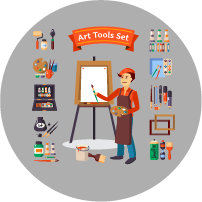
\includegraphics[width=4cm, height=4cm]{Sketch Artists}
  \caption{Digital Board Marker Application: Sketch Artists}
\end{figure}

\bigskip

\subsection{Industrial Presentations}
Digital board marker can be helpful in industrial presentation so that if any person cannot appear at the particular time, that person can watch the recorded (storage efficient) presentation later. So industry will also have less use of its resources.

\bigskip

\begin{figure}[h]
  \centering
  
\includegraphics[width=5cm, height=3cm]{Industry}
  \caption{Digital Board Marker Application: Industrial Presentations}
\end{figure}

\bigskip













 % Introduction 

% Chapter 2

\chapter{Literature Review} % Write in your own chapter title
\label{Chapter2}
\lhead{Chapter 2. \emph{Literature Review}} % Write in your own chapter title to set the page header

\section{Literature Review}
Have you ever wanted as a student that if you can take the lecture again because you missed it last time because of some mishap or the concepts delivered in that lecture was too hard to grasp immediately and you wanted to discuss them later with other people but you could not remember most of it because you cannot jot down each and every thing? One time or another we all have been there. To achieve this goal many techniques were used providing notes or recording lectures and later providing them to all the students but since every thing has its own pros and cons so first we have to make sure that these facilities are either productive or destructive many researches has done to support the idea of use of revolutionized lecture systems different techniques were used to achieve this goal but we will get back to those techniques later. First we have to see the use of these facilities is beneficial or not.
The use of video lectures in educational institution is considered as an essential source because students can't pay complete attention in class whole the time. It is important to provide an alternative as good as possible that's why video lectures pay a huge role. Web-based lecture technologies are being used increasingly in higher education. One widely-used method is the recording of lectures delivered during face-to-face teaching of on-campus courses. The recordings are subsequently made available to students on-line and have been variously referred to as lecture capture, video podcasts, and Lectopia. We examined the literature on lecture recordings for on-campus courses from the perspective of students, lecturers, and the institution. Institutions receive pressure from a range of sources to implement web-based technologies, including from students and financial imperatives, but the selection of appropriate technologies must reflect the vision the institution holds. Students are positive about the availability of lecture recordings. They make significant use of the recordings, and the recordings have some demonstrated benefits to student learning outcomes. Lecturers recognize the benefits of lecture recordings for students and themselves, but also perceive several potential disadvantages, such as its negative effect on attendance and engagement, and restricting the style and structure of lectures. It is concluded that the positives of lecture recordings outweigh the negatives and its continued use in higher education is recommended. However, further research is needed to evaluate lecture recordings in different contexts and to develop approaches that enhance its effectiveness.\cite{OCallaghan2017}\\
Then a research team decided to see the impact of flipped classroom on students and their growth.A flipped classroom is an instructional strategy and a type of blended learning that reverses the traditional learning environment by delivering instructional content, often online, outside of the classroom. It moves activities, including those that may have traditionally been considered homework, into the classroom.\\
The meta-analysis comparing these 29 traditional flipped interventions in relation to student achievement showed an overall significant effect in favor of the flipped classroom over traditional lecturing (Hedges' g =0.289, 95\% CI [0.165, 0.414], p< .001). A moderator analysis showed that the effect of the flipped classroom was further enhanced when instructors offered a brief review at the start of face-to-face classes.\\
They calculated students learning rate by means of hedges' g which tells whether the impact of flipped classroom is positive or negative and the impact of flipped classrooms was mostly positive the learning rate of students increased and passing rate of class also increased. That means flipped classroom was much more good than traditional classrooms. They used number of samples to make sure the conclusion and in majority of samples result was same that flipped classroom are an innovation in educational institutions.\cite{Lo2019}\\
Then we have to see the effects of prior knowledge on students because different approaches can be used to increase the growth rate of students so it can be a positive approach. A research was conducted to analyze these results and a research paper was published as a result of data set in 2019. That paper shows how a student behaves in general if lecture related material or videos are provided first. They categorized students in two categories the one with low prior knowledge LK and the one with high prior knowledge HK then they used these samples to examine the behavior of students in each sample to check with prior knowledge how many times students does what actions like start over rewind a video after the lecture so that they can see how much interest students are showing and how these videos are helping them in their studies and students with high prior knowledge had more potential and passed their exams with more marks then LK.\\
The purpose of this analysis was to answer the following questions:\\
1. Does prior knowledge affect students’ engagement level of viewing video lectures?\\
2. Does prior knowledge affect students’ strategies used for viewing video lectures?\\
3. Does prior knowledge affect students’ learning performance when learning from video lectures?\\
4. Does prior knowledge affect learners’ attitudes toward video lectures?\\
Effect was positive for all the students with high prior knowledge they have to do less effort.\cite{Li2019}\\
Then a system was made to use the video lectures but to make them more effective it was based on the brainwaves of learner. This system was made for the benefit of students so that they can learn everything on the basis of their attention. Video lectures are common but this system records the patches of video based on the attention of students on brain signals that if they missed any part which was important they can watch it later and know that they missed this thing.\cite{Lin2019}
A study was done in 2019 to see the benefit of recorded lectures that they are decreasing the burden off for both students and teachers and how they are helpful for them. This study was done for the students of pharmacy to see their response and performance if they get recorded lectures or not study shows that students have more storage space like a storage device when we tell them they can have the recorded lectures so they can focus on other things which are more productive and it will increase their performance because now they have a medium for later use so that they can use their brain for other important things study shows how human minds works as a storage space if we tell them that they will not get recorded lectures they will save their storage space to absorb the lecture and fully remind so that later on they don't get any difficulty but in spite of helping them it will stop them from growing.\cite{Patel2019}\\
Sometimes customized things are better in educational system because everyone has their own method of teaching and learning for that purpose video lectures are used but what if we change the way of delivery of those lectures by marking the timeline so that students know which part is important for them for that purpose a research was done and published in 2019. That research shows how a marked timeline of a video lecture affects the behavior of students they took two groups of students as sample and showed one group conventional video of lectures and other group the marked timeline video and the experiment showed how the behavior of students who were shown a marked timeline with topics or keynotes was different they clicked less on timeline and their pattern of clicking the timeline was almost same and later on they performed well on that test or quiz held from that video because of the interactive timeline the behavior of students changes and the feel more open to learn and explore.\cite{Pimentel2019}\\
Now if we are using video lectures then we have to see the effects on audience on them. For that purpose a study was conducted on the effects of video lectures on university students and how they spend their time on them. This study shows how online lectures plays a good role in the learning of students they provided online videos to students with lectures and recorded their time spent on lecture and video lectures and study showed students uses online videos as a substitute of lectures and it is a positive thing to learn those who spent time in lecture have same learning to those who spent equal time on video lectures.\cite{Meehan2019}\\
Video lectures was invented because student cannot take notes about each and everything in lecture and they miss things. A research was conducted to see how it can be helpful to take effective notes in classroom. This research focuses on the behavior of students while taking notes typically students note everything written on board and a very few of them write on their own to find links between lecture and their learning and this thing is good for the growth of any student but a few does it because a student brain thinks what a teacher is writing on the board is most important and after that what he is saying is important very few thinks what they are learning and thats whats needed in notes taking for a productive notes taking of students.\cite{Iannone2019}\\
Online lectures have their own cons but they can be recovered by a number of things a research was conducted in 2018 to study the effect of these facilitation in online courses. This study shows how some strategies work for the students interaction and interest in an online course teacher uses different strategies to engage students in an online course because it is so easy for students to just let it go they can just quit it so all the teachers around the globe uses some strategies to develop the interest of student and in this study they examined 13 strategies to see the behavior of students.\\
1. Instructor presence\\
2. Instructor Connectedness\\
3. Engagement \\
4. Learning\\
All 13 strategies constructs around these four factors. and these strategies are:\\
1. Video based instructor introduction (e.g., Voicethread, Animoto, Camtasia)\\
2. Video based course orientation (e.g., recording using Camtasia, screencast o matic)\\
3. Able to contact the instructor in multiple ways (contact the instructor forum, email, phone, 4. virtual office hours)\\
5. Instructors timely response to questions (e.g., within 24 to 48 h) via forums, email\\
6. Instructors weekly announcements to the class (e.g. every Monday via announcement forum, email)\\
7. Instructor created content in the form of short videos/multimedia (e.g., Camtasia, articulate modules)\\
8. Instructor being present in the discussion forums (e.g., refers to students by name, responds to students posts)\\
9. Instructor providing timely feedback on assignments/projects (e.g., within 7days)\\
10. Instructor providing feedback using various modalities (e.g., text, audio, video, and visuals) on assignments/projects\\
11. Instructors personal response to student reflections (e.g., via journals to questions on benefits/challenges\\
12. Instructors use of various features in synchronous sessions to interact with students (e.g., polls, emoticons, whiteboard, text, or audio and video chat)\\
13. Interactive visual syllabi of the course (e.g., includes visual of the instructor and other interactive components)\cite{Martin2018}\\
Online learning environments use different approaches to convey their information to their audience but when learning is most important thing in an online environment then we can use learning centered environment it uses number of factors to increase the learning rate. The design of online course materials is rarely informed by learning theories or their pedagogical implications. The goal of this research was to develop, implement and assess a virtual learning environment (VLE), SOFIAA, which was designed using the cognitive apprenticeship model (CAM), a pedagogical model based on learning-centered theory. We present an instructional design case study that reveals the steps taken to improve student performance in a master’s level blended learning course on program evaluation. The case study documents four phases of improving on-line instruction in program evaluation, starting with Online Course Materials (OCM) that contained resources and information required to complete team field projects. In phase 1, quantitative analyses revealed that there was improvement of student test scores using the OCM, however, qualitative analyses of think-aloud sessions found that students failed to attain key course objectives. In phase 2, a team of experts reviewed the materials and suggested ways to improve opportunities for student learning. In phase 3, a (VLE) was designed based on the results of phase 2 using a reconceptualization of CAM as a design model. In phase 4, the VLE was validated using experts’ appraisal of content and presentation, and student achievement, which indicated that use of the VLE led to significant improvement in learning over use of OCM. The design process is discussed in terms of a reconceptualization of CAM as a general strategy for instructional design that can be used to improve both the content and quality of online course materials.\cite{Garcia-Cabrero2018}\\
A study was conducted on the note taking quality of students in 2018. Many Students are terrible note takers who record just one third of a lecture's important points in their notes. This is not a good practice, because the number of lesson points recorded in notes is directly proportional to student's achievement. Moreover, both recording notes and the continuous review of notes are beneficial. The authors offer instructors a menu of research-based advice for increasing effectively student note taking: provide complete notes, partial notes, note- taking cues, represent the lesson, pauses and revision opportunities, control laptop usage, control "cyber-slacking", use slides effectively, and teach notes-taking skills to students. Authors also suggest ways to help students change their notes during the note-review process and select, organize, associate, and regulate their notes effectively to success. This study shows how notes taking helps student and how student are not good with it but we have to do something to improve it so their are some things or remedies we can do to improve it because notes are basically most essential thing for a student to get through the exams.\cite{Kiewra2018}\\
Engagement of students increase student's satisfaction, enhances student's motivation to learn, reduces the isolation sense, and improves performance of each student in online course. A survey-based research study was conducted to examine student's perception on different engagement strategies which are used in online courses based on  an interaction framework MOOR. 38 item survey was completed by one hundred and fifty-five students which was based on engagement strategies of learner-to-learner, learner-to-instructor and learner-to-content. The most valued engagement strategy was Learner-to-instructor among the three categories .In the learner-to-learner category the engagement strategy rated the most was Icebreaker/introduction discussions and working collaboratively using online communication, whereas in learner to instructor category sending regular announcements or email reminders and providing grading rubrics for all assignments were rated most beneficial. In the learner-content category, students mentioned working on real-world projects and having discussions with structured or guiding questions were the most beneficial. This study also analyzed the effects of age, gender and years of online learning experience differences on student's perception of engagement strategies. The results of the study have involved conclusion for online instructors, instructional designers, and administrators who wish to enhance engagement in the online courses. Basically, this paper shows how engagement matters in an online course because online courses can be a complete waste if we don't do it properly and study properly in it includes engagement of the student that he can follow the course as the instructor is teaching and what strategies we should use to engage a student in an online course. \cite{Martin2018(2)}\\
A study was conducted to analyze the behavior of students in massive open online courses (MOOCS) like how students show their confusion about things and how to improve that model so that student will have less confusion because more confusion creates less retention so if we can provide things in a way that students would have less confusion then they will focus on much more creativity and new ideas so in MOOCS we have to reduce the reasons of confusion as much as possible.\cite{Yang2016}\\
Discussion forums are also held in MOOCS and the odds of confusion is much more greater than the online courses because different people are giving different views and discussing them which can lead to confusion among the learners. The construction and destruction both are equally possible in discussion forums because confusion can change the discussion entirely and to prove that point a study was conducted in 2015 to examine the effects of confusion in MOOCS.\cite{Yang2015}\\
Then we have to see the patterns on which a student view and understand a video lecture for that cause a study was conducted in 2016 to see if their is any relationship between video lecture pattern and student perception of watching them and results shows that their were certain patterns on which a student watches an online lecture.\cite{Giannakos2016}\\
We have discussed all the pros and cons of video lectures and how to make them more efficient for the students but what if the quality or source of video becomes a problem video lectures takes a lot of space and a lot of speed is needed to stream them smoothly. If they are not streamed smoothly it is almost impossible to understand a lecture. A human mind loses interest in something after 2 seconds if its buffering and we feel angry and irritated so how can we focus on a video lecture which buffers after every 1 minute or even seconds. For that purpose different techniques were introduced to optimized the video size or quality to stream it smoothly. A good quality video is hard to stream but an average quality video can be streamed easily but what if we cannot compromise on quality. It is a seesaw but we have to balance both quality and space.\\
Automated video recording system was introduced in 2010 by a researcher in his paper. A PTZ camera was used in this study to capture the video lecture instead of a cameraman this camera acts as a cameraman and tracks the screen and lecturer and starts recording the lecture.\cite{Chou2010} 
The cons of this system was it provides the simple video and the streaming issue remains the same even if a student downloads every lecture he may need a lot of space to save them because 1 lecture of one hour can take space up to 1 GB.\\
Another technique to increase the quality and understanding of video lecture was introduced in 2017 by research team in their research paper. This technique captures video from different angles and multi-stream them. The approach was to use multiple cameras to get same scenes from different angles and stream the most suitable. The movements and actions of cameras were synchronized all the cameras captures the video at the same time. It increased the canvas of video lecture at that time later this technique was used in many gaming engines too. \cite{Carlsson2017} The con of this technique was that to capture a scene which is static in case of lecture video use of multiple cameras was expensive and quality wasn't even that much better.\\
A tracker named Gal Tracker was also introduced in 2013 by a researcher. The use of this tracker was to optimize the lecture recording. It captures the lecture in real time environment also called real time lecture capturing. It captures all the important parts of lecture and creates slides of lecture according which can be later distributed among the users.\cite{Gonzalez-Agulla2013} Again the issue is it can not capture all the important points given that it works on cues it can only capture a certain type of info and if something new comes it might fail in that environment. Its basically optimizing the lecture notes not lecture videos but trying to provide the same feature.\\
In MOOCS platform it is essential to provide videos but many people are working how to optimize them as much as possible and their type of optimization depends on how user can interact with video lectures. A research was conducted in 2015 to check how user interacts with single and multi streamed videos and their behavior on them. They also tested how it will help if a user can stream two videos at the same time.\cite{Renz2015} This statistical data from this research can be used to improve many new video streaming engines.\\
Since many people are streaming videos worldwide it is a wast field to compress these files but but compression can cause loss of data. To minimize the loss of data as much as possible different techniques of compression are used throughout the years. Wavelet transform is an efficient method to compress videos but in 2011 a research was conducted to achieve video compression algorithm using frame difference approach. This technique was to discard unimportant frames and keep the ones which can be important now the factors which decides whether the frame is important or not can be compression performance or frame change from previous one if its too minor it can be discarded. This technique was tested on many videos and the results were positive it can optimize the video size upto 3 percent and it's a big thing when we stream a 2 GB HD video with less amount of bandwidth.\cite{AlAni2011}
As we discussed earlier video compression is a wast field so here is another technique to compress a video: in 1992 an algorithm was developed to compress a video by MPEG video compression algorithm. The major focus of this algorithm is based on two techniques: block based motion compensation for the reduction of the temporal redundancy and transform domain based compression for the reduction of spatial redundancy. Motion compensation techniques are used with both interpolative and predictive techniques. The prediction error signal is further compressed with spatial redundancy reduction (DCT). This algorithm changed the video about 1.5Mbit/s.\cite{LeGall1992}\\
As we discussed different compression algorithms but they have some cons when we compress a video we compromise its quality a data loss is possible. There are some techniques which focuses on video compression as well as preserving the quality or resolution of video one of them was presented in 2016 which focuses on multi-level optimization of encoding to balance video compression and retention of 8k resolution. A paper was presented for this technique. This Paper is focused on providing better quality videos after compression by using some factors and techniques. This paper presents a technique that aimed to achieve an efficient balance between video compression using H.265 protocol and retention of 8K resolution. The study implements multi-level of optimization in the encoding process using H.265 where we can see JPEG2000 standards play an important role. The study also uses a novel concept of orthogonal projection that manages pixels metadata required in every frame transition by using motion compensation. By using multiple file formats of 30 video datasets, the outcome of the study is found to be achieving approximately 49 percent of increase in data quality and around 59 percent of enhancement in video compression in comparison to the former techniques of HEVC-based video compression which are most commonly used techniques.\cite{Murthy2016}\\
We saw how video lectures are helpful for learning and growth of students, how different video recording techniques are used to provide video lectures or notes, how compression of videos is important and how quality is important. We discussed different techniques and studies to achieve and justify all the goals. These techniques are not perfect but they are achieving the goal somehow "provide video lectures with ease". Ease can be considered as less space hogging and less bandwidth usage and still stream the lecture as possible. But first we have to see one thing to capture these lectures we have to change the environment of a classroom and we have to see either these changes are good or bad for classroom environment some studies were conducted to see the behavior of students towards these changes and the studies have shown positive result students were much attentive in lecture because they don't have to jot down the lecture they can focus on the concept because now they can access those lectures later on if wanted.\cite{Brooks2014}\cite{Chen2015}\cite{Barokas2010}\\
After discussing all the pros and cons of video lectures, availability of video lectures and techniques to make it easier. We are going to discuss another technique introduced by us. Compression may cause loss of data and quality may increase the space or bandwidth issue. To overcome this issue we are introducing DBM(digital board marker) this technique uses coordinate information to generate a video later on. DBM erases all the noise from video and chooses to save the information written on board or screen and audio of instructor. It draws a virtual plain on board and saves the coordinate information with respect to time in a customized file which can be later used to generate the video of board on our customized player integrated in web app and desktop application with a speed less than 2.5Kb. Which is much less than all the compression techniques used. So, DBM is solving all the compression problems for lecture videos and providing video lectures which is essential for the growth of student's learning.
 

 
\section{Comparison Table}

\begin{sideways}
\centering
\begin{tabularx}{1.5\textwidth} { 
  | >{\raggedright\arraybackslash}X 
  | >{\centering\arraybackslash}X | >{\centering\arraybackslash}X | >{\centering\arraybackslash}X | >{\raggedleft\arraybackslash}X | }
 \hline
\bfseries{Name} & \bfseries{Support Video Lectures} &\bfseries{Provide Video Lectures} &\bfseries{Technique to Provide Video Lectures} & \bfseries{Video Optimization}  \\
\hline
Muti-level optimization in encoding to balance video compression and retention of 8k resolution
&
&
&
&
\\
\hline
Muti-level optimization in encoding to balance video compression and retention of 8k resolution
&
&
&
&
\\
\hline

Muti-level optimization in encoding to balance video compression and retention of 8k resolution
&
&
&
&
\\
\hline

Muti-level optimization in encoding to balance video compression and retention of 8k resolution
&
&
&
&
\\
\hline



\end{tabularx}
\end{sideways}


\begin{sideways}
\centering
\begin{tabularx}{1.5\textwidth} { 
  | >{\raggedright\arraybackslash}X 
  | >{\centering\arraybackslash}X | >{\centering\arraybackslash}X | >{\centering\arraybackslash}X | >{\raggedleft\arraybackslash}X | }
 \hline
\bfseries{Name} & \bfseries{Support Video Lectures} &\bfseries{Provide Video Lectures} &\bfseries{Technique to Provide Video Lectures} & \bfseries{Video Optimization}  \\
\hline
Muti-level optimization in encoding to balance video compression and retention of 8k resolution
&
&
&
&
\\
\hline
Muti-level optimization in encoding to balance video compression and retention of 8k resolution
&
&
&
&
\\
\hline

Muti-level optimization in encoding to balance video compression and retention of 8k resolution
&
&
&
&
\\
\hline

Muti-level optimization in encoding to balance video compression and retention of 8k resolution
&
&
&
&
\\
\hline



\end{tabularx}
\end{sideways}

\section{Shortcomings in Existing Systems}





 % What to Write 

% Chapter 3

\chapter{Proposed Methodology} % Write in your own chapter title
\label{Chapter3}
\lhead{Chapter 3. \emph{Proposed Methodology}} % Write in your own chapter title to set the page header

\section{Proposed Solution}
The proposed system focuses on size efficiency of the output video. System acts well in the environment where there is storage issue and bandwidth issue in terms of internet transfer rate. Ultra-durability makes the system more portable to use and more reliable to handle. Re-positionable cameras make the system able to work well in different canvas sizes i.e. size of writing board. System automates the process of video compression technique. Video of the lecture is not recorded as it as video format rather only the important data is extracted. By utilizing the stereo vision and high-speed cameras and low wireless latency, video animation and sound quality is maintained in noisy environment as well. 


\section{General Flow}
The system consists on several modules and deliverables one of which is controller application. This application is quite important because it include major functionalities and complex image processing algorithms. Furthermore, the instructor in mainly connected to the controller application so that he/she is controlling the recording of lecture i.e. he can start, pause or stop the recording. After the lecture is recorded, he can replay the lecture for any further changes. When the lecture is finally uploaded to central computer, students can play lecture online or save the lecture file in .dbm(file extension) extension to watch later.\\ Offline player is also one of the major modules of the project. It plays the downloaded lecture file just like video player. Learning management system is the online platform where all uploaded online lecture hierarchy is accessible. It is a comprehensive management system designed by placing the convenience of instructor and student in focus. Reliability, security and quality are the top priorities.
A simple visual of the working of system can be seen below

\begin{figure}[h]
  \centering
  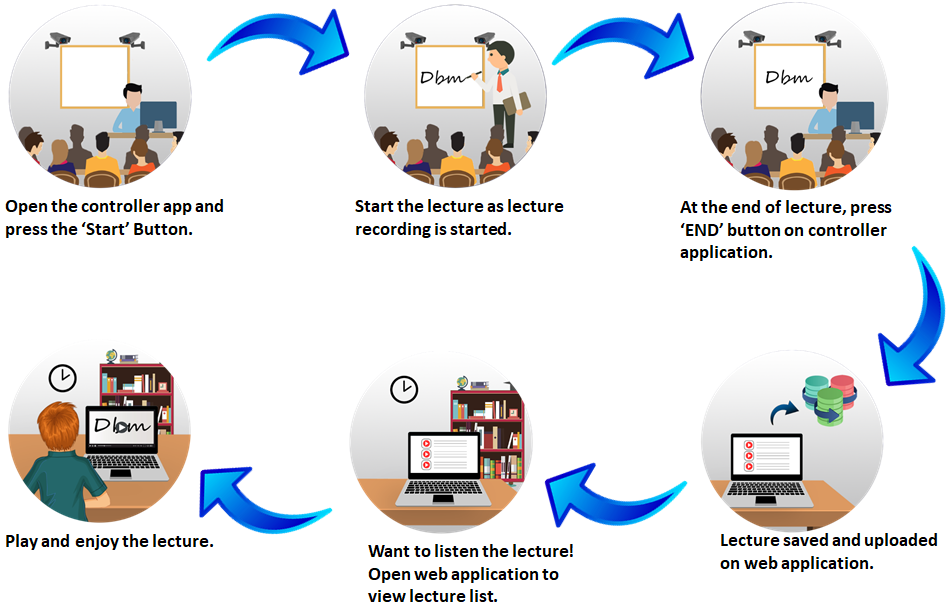
\includegraphics[width=13cm, height=8cm]{Workflow}
  \caption{General Flow of the Project}
\end{figure}

\section{General Proposed Model}
General working model of the system can be seen below

\begin{figure}[h]
  \centering
  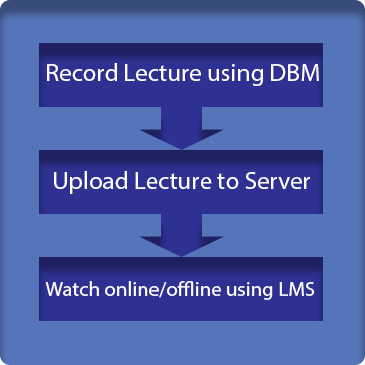
\includegraphics[width=14cm, height=9cm]{General Model}
  \caption{General Methodology View of the System}
\end{figure}

\newpage
%\bigskip

\section{Formulas Used}
\begin{longtable}{|>{\raggedright\arraybackslash}p{3cm}|p{4cm}|p{7cm}|}
\hline
\textbf{Descriptor} & \textbf{Explanation} & \textbf{Formula}\\
\hline
% Row 1 start
\vspace{0pt}\large Euler Angles Rotation Matrices &
Transpose of the fixed-axis matrix. Used in orientation extraction of Board Marker & 
\begin{minipage}{.3\textwidth}
      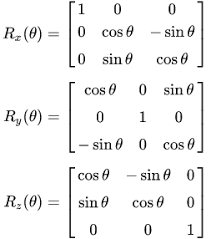
\includegraphics[width=\linewidth, height=50mm, valign=T]{EulerAngles}
\end{minipage}
\\
% Row 1 end
\hline

% Row 1 start
\vspace{0pt}\large Quaternion to Euler conversion &
Used in Marker calibration when an offset is given in particular dimension. & 
\bigskip
\begin{minipage}{.3\textwidth}
      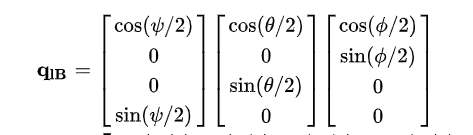
\includegraphics[width=65mm, height=30mm]{Quaternion to Euler conversion}
\end{minipage}
\\
% Row 1 end
\hline



% Row 1 start
\vspace{0pt}\large Euclidean distance formula &
Used to compute the distance in one-dimension. & 
\begin{minipage}{.3\textwidth}
      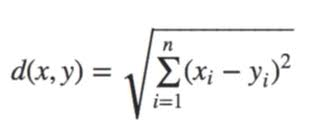
\includegraphics[width=60mm, height=30mm]{Euclidean distance formula}
\end{minipage}
\\
% Row 1 end
\hline


% Row 1 start
\vspace{0pt}\large Equation of line in slope-intercept form &
Used to draw lines and get relative position of Marker with respect to cameras. & 
\bigskip

\begin{minipage}{.3\textwidth}
      
\includegraphics[width=60mm, height=10mm]{slope-intercept form}
\end{minipage}
\\
% Row 1 end
\hline



\caption{Formulae and Equations used}
\end{longtable}

\section{Use-Case Diagrams}
To describe the system requirements, use-case diagrams in form of simple user interaction are detailed below
\subsection{Controller Application}
The main end user of controller application is the class instructor or teacher. Teacher use the controller application in
\begin{itemize}

\item Calibrating hardware
\item Record the Lecture
\item Live Stream Lecture
\item Generate Lecture File and annotate it
\item Send Lecture file to Central Server


\end{itemize}

\begin{figure}[h]
  \centering
  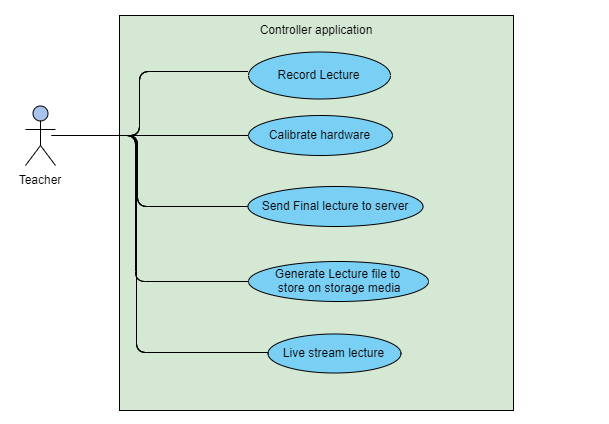
\includegraphics[width=13cm, height=12cm]{ControllerApplication}
  \caption{Use-case Diagram of Controller Application}
\end{figure}


\subsection{Player Application}
Just like media player, the player application plays the lecture. Common end user of Player Application is student. Teacher and Student are end users of controller application. Typical actions of Player application are:

\begin{itemize}

\item View Playlist
\item Play Lecture
\item Live Stream Lecture


\end{itemize}

\bigskip

\begin{figure}[h]
  \centering
  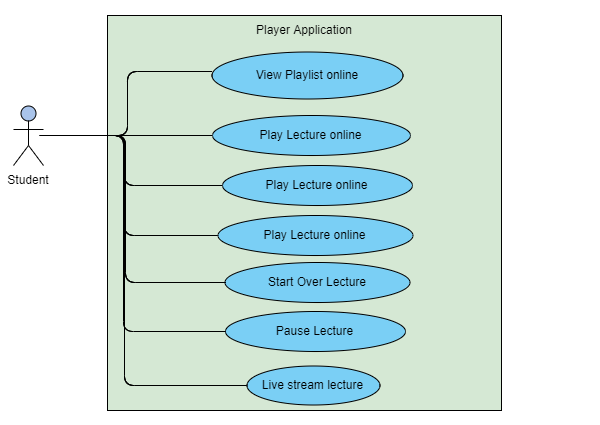
\includegraphics[width=13cm, height=14cm]{PlayerApplication}
  \caption{Use-case Diagram of Player Application}
\end{figure}

\newpage
\subsection{LMS Web Application}
LMS application is major module in terms of accessibility. Students, Teachers and administration can have access to this module simultaneously. LMS functionality is sub-divided into following different users:

\begin{itemize}

\item Admin, who manages the institute.
\item Teacher, who manages students
\item Users, who are students

\end{itemize}

\newpage
\begin{figure}[h]
  \centering
  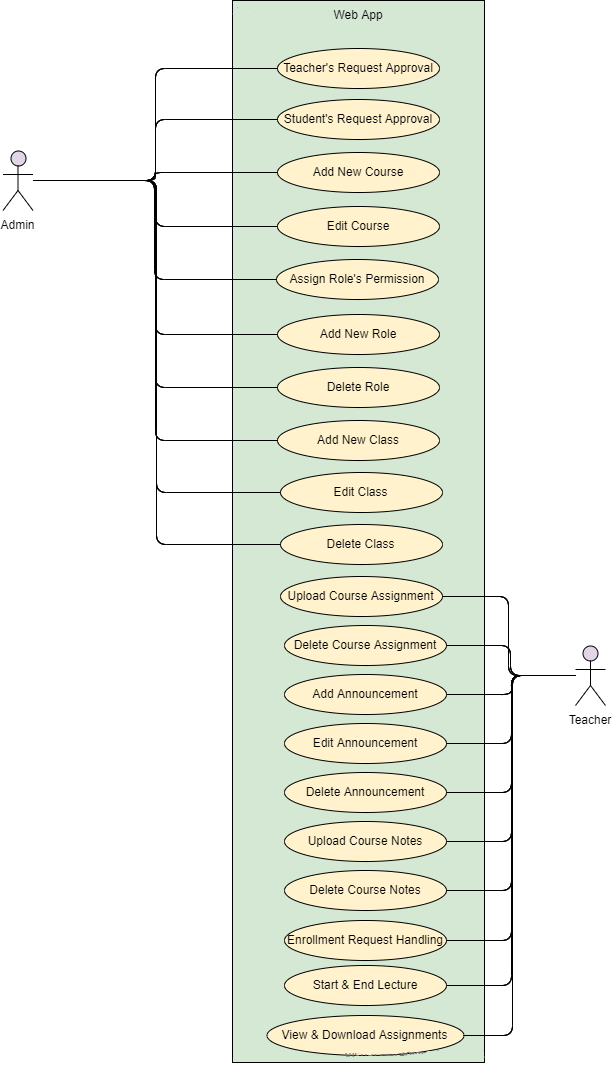
\includegraphics[width=15cm, height=20cm]{DBMUseCaseWebAppPart1}
  \caption{Use-case Diagram of LMS Web Application Part-I}
\end{figure}

\newpage

\begin{figure}[h]
  \centering
  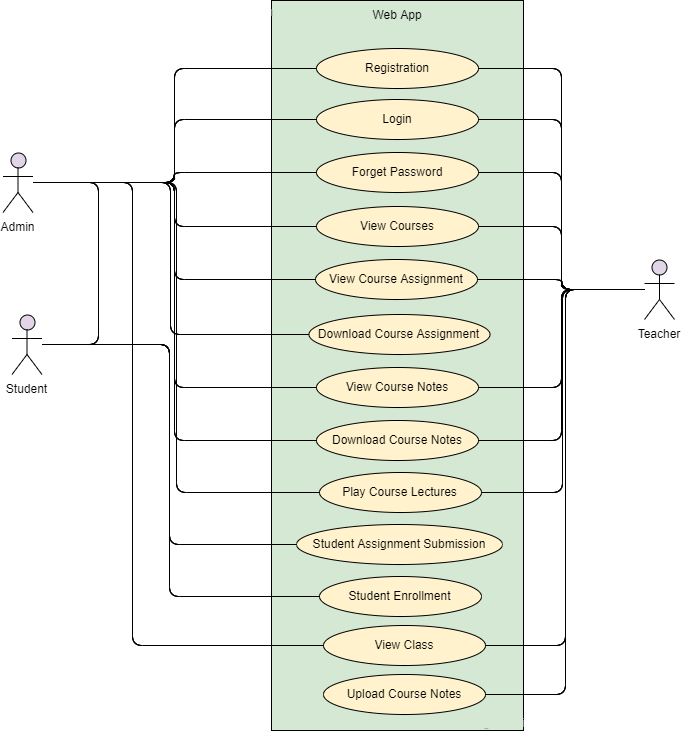
\includegraphics[width=15cm, height=14cm]{DBMUseCaseWebAppPart2}
  \caption{Use-case Diagram of LMS Web Application Part-II}
\end{figure}


\section{Use Cases(Web App)}
\subsection{Use Case UC-1: User Registration}
\textbf{Stakeholders: } University, Educational Institutes \\
\textbf{Primary Actors: } Student, Teacher \\
\textbf{Post Condition: }\\
User data successfully sent to admin request approval page.\\
\textbf{Main Success Scenario: }
\begin{enumerate}
\item User wants to register.
\item User clicks on the Register link from the main Page header.
\item Registration page will be open by the system.
\item User will enter First Name, Last Name, Email, CNIC, Password and Date of birth.
\item User will select Institute name from the select list.
\item User select whether he is teacher or a student from the select list.
\item If user is student then system will show a input box for student registration No.
\item Student will enter his registration Number.
\item User clicks the \textbf{Sign Up} button.
\item System then send data to the Admin Request Approval page for the student request approval. 
\end{enumerate}
\textbf{Alternative Flow: }\\
\\
*a. At any time system fails.
\begin{enumerate}
\item User must check the internet connectivity.
\item Restart the browser and try again.
\item Try after sometime might be servers are down.
\end{enumerate}
3a. Registration page is not opened.
\begin{enumerate}
\item Refresh the browser.
\item Reload the page and try again.
\end{enumerate}
4a. User entered the invalid First Name, Last Name.
\begin{enumerate}
\item System will show the error message.
\item System will ask the user to enter the data again.
\end{enumerate}
4b. User entered the invalid Email.
\begin{enumerate}
\item System will show the error message.
\item System will ask the user to enter the data again.
\end{enumerate}
4c. User entered the invalid CNIC.
\begin{enumerate}
\item System will show the error message.
\item System will ask the user to enter the data again.
\end{enumerate}
4d. User entered the invalid Registration No.
\begin{enumerate}
\item System will show the error message.
\item System will ask the user to enter the data again.
\end{enumerate}
4e. User entered the invalid Date of birth.
\begin{enumerate}
\item System will show the error message.
\item System will ask the user to enter the data again.
\end{enumerate}
8a. Student entered the registration No. in invalid format.
\begin{enumerate}
\item System will show the error message.
\item System will ask the user to enter the data again.
\end{enumerate}
9a. Required fields are empty.
\begin{enumerate}
\item System will show the error message.
\item System will ask the user to complete all the required fields.
\end{enumerate}
9b. Sign Up button is not clicked.
\begin{enumerate}
\item information will be saved as a draft for later use.
\end{enumerate}
\textbf{Frequency of Occurrence:}\\
One time per user.



\subsection{Use Case UC-2: User Login}
\textbf{Stakeholders: } University, Educational Institutes \\
\textbf{Primary Actors: } Student, Teacher, Admin \\
\textbf{Preconditions: }
\begin{itemize}
\item User is approved by the admin.
\item User is identified and authenticated.
\item User's record is saved.
\end{itemize}
\textbf{Post Condition: }
\begin{itemize}
\item User is logged in into the system.
\item User has access to different functionality of the system.
\end{itemize}

\textbf{Main Success Scenario:}
\begin{enumerate}
\item User wants to login.
\item User clicked on the login link to access the login page from the header.
\item System open the login page for the user.
\item User enter email address along with the password.
\item User clicked the \textbf{Sign In} button.
\item System validates the user email and password.
\item System will redirect the user to next page.
\end{enumerate}
\textbf{Alternative Flows:}\\
\\
*a. At any time, system fails.
\begin{enumerate}
\item User must check the internet connectivity.
\item Restart the browser and try again.
\item Try after sometime might be servers are down.
\end{enumerate}
3a. Login page is not opened.
\begin{enumerate}
\item Refresh the browser.
\item Reload the page and try again.
\end{enumerate}
4a. User entered invalid email and password.
\begin{enumerate}
\item System will show the error message.
\item System will ask the user to enter the data again.
\end{enumerate}
5a. Required fields are empty.
\begin{enumerate}
\item System will show the error message.
\item System will ask the user to complete all the required fields.
\end{enumerate}
6a. User is not identified or authenticated.
\begin{enumerate}
\item System will show error message.
\item System will ask the user to register yourself first.
\end{enumerate}
\textbf{Frequency of Occurrence:}\\
Whenever the user wants to login.





\subsection{Use Case UC-3: Teacher's Requests Approval/Disapproval}
\textbf{Stakeholders: } University, Educational Institutes \\
\textbf{Primary Actors: } Admin \\
\textbf{Preconditions:}
\begin{itemize}
\item Admin is logged in the system..
\item Admin is identified and authenticated.
\end{itemize}
\textbf{Post Conditions: }
\begin{itemize}
\item Requests are approved / disapproved.
\item On approval / disapproval, Email is sent to the teacher.
\item Teachers can login to the system.
\end{itemize}
\textbf{Main Success Scenario:}
\begin{enumerate}
\item Admin wants to handle the requests of teachers.
\item Admin clicks on the Teacher requests approval link from the header.
\item System open the \textbf{teachers request approval} page for the admin.
\item Admin can see the list of all the requests of teachers.
\item Admin clicks on the \textbf{Approve} button for approval of request.
\item System send the approval email to that teacher.
\item System show the success message to admin that email is sent.
\item System saves the record of the teacher.
\item System removes the request from the page.
\item Admin disapprove the request of a teacher by clicking on \textbf{Disapprove} button.
\item System delete that temporary record of the user.
\item System send an disapproval email to the teacher.
\item System show the success message to admin that email is sent.
\item System removes the request from the page.
\end{enumerate}
\textbf{Alternative Flows:}\\
\\
*a. At any time, system fails.
\begin{enumerate}
\item User must check the internet connectivity.
\item Restart the browser and try again.
\item Try after sometime might be servers are down.
\end{enumerate}
3a. Page is not opened.
\begin{enumerate}
\item Refresh the browser.
\item Reload the page and try again.
\end{enumerate}
5a. Approve button is not working properly.
\begin{enumerate}
\item Admin must have to refresh the page.
\item Restart the browser and try again.
\item May be some backend issue, resolve that issue.
\end{enumerate}
6-7a. Email is not sent to the teacher.
\begin{enumerate}
\item Admin must again approve the request of teacher.
\item May be some backend issue, resolve that issue.
\end{enumerate}
8-9a. Request is not removed from the page and record is unsaved.
\begin{enumerate}
\item Admin must again approve the request of teacher.
\item May be some backend issue, resolve that issue.
\end{enumerate}
10a. Disapprove button is not working properly.
\begin{enumerate}
\item Admin must have to refresh the page.
\item Restart the browser and try again.
\item May be some backend issue, resolve that issue.
\end{enumerate}
12-13a. Email is not sent to the teacher.
\begin{enumerate}
\item Admin must again approve the request of teacher.
\item May be some backend issue, resolve that issue.
\end{enumerate}
14a. Request is not removed from the page.
\begin{enumerate}
\item Admin must again approve the request of teacher.
\item May be some backend issue, resolve that issue.
\end{enumerate}
\textbf{Frequency of Occurrence:}\\
Whenever the requests appear on the page.
\\
\textbf{Open Issues:}\\
What will happen if admin has mistakenly approve or disapprove the request of teacher?


\subsection{Use Case UC-4: Student's Requests Approval/Disapprovals}
\textbf{Stakeholders: } University, Educational Institutes \\
\textbf{Primary Actors: } Admin \\
\textbf{Preconditions:}
\begin{itemize}
\item Admin is logged in the system..
\item Admin is identified and authenticated.
\end{itemize}
\textbf{Post Conditions: }
\begin{itemize}
\item Requests are approved / disapproved.
\item On approval / disapproval, Email is sent to the student.
\item Students can login to the system.
\end{itemize}
\textbf{Main Success Scenario:}
\begin{enumerate}
\item Admin wants to handle the requests of students.
\item Admin clicks on the student requests approval link from the header.
\item System open the \textbf{Students Request Approval} page for the admin.
\item Admin can see the list of all the request of students.
\item Admin clicks on the \textbf{Approve} button for approval of request.
\item System send the approval email to that student.
\item System show the success message to admin that email is sent.
\item System saves the record of the student.
\item System removes the request from the page.
\item Admin disapprove the request of a student by clicking on \textbf{disapprove} button.
\item System delete that temporary record of the user.
\item System send an disapproval email to the student.
\item System show the success message to admin that email is sent.
\item System removes the request from the page.
\end{enumerate}
\textbf{Alternative Flows:}\\
\\
*a. At any time, system fails.
\begin{enumerate}
\item User must check the internet connectivity.
\item Restart the browser and try again.
\item Try after sometime might be servers are down.
\end{enumerate}
3a. Page is not opened.
\begin{enumerate}
\item Refresh the browser.
\item Reload the page and try again.
\end{enumerate}
5a. Approve button is not working properly.
\begin{enumerate}
\item Admin must have to refresh the page.
\item Restart the browser and try again.
\item May be some backend issue, resolve that issue.
\end{enumerate}
6-7a. Email is not sent to the student.
\begin{enumerate}
\item Admin must again approve the request of student.
\item May be some backend issue, resolve that issue.
\end{enumerate}
8-9a. Request is not removed from the page and record is unsaved.
\begin{enumerate}
\item Admin must again approve the request of student.
\item May be some backend issue, resolve that issue.
\end{enumerate}
10a. Disapprove button is not working properly.
\begin{enumerate}
\item Admin must have to refresh the page.
\item Restart the browser and try again.
\item May be some backend issue, resolve that issue.
\end{enumerate}
12-13a. Email is not sent to the teacher.
\begin{enumerate}
\item Admin must again approve the request of student.
\item May be some backend issue, resolve that issue.
\end{enumerate}
14a. Request is not removed from the page.
\begin{enumerate}
\item Admin must again approve the request of student.
\item May be some backend issue, resolve that issue.
\end{enumerate}
\textbf{Frequency of Occurrence:}\\
Whenever the admin get requests from students.
\\
\textbf{Open Issues:}\\
What will happen if admin has mistakenly approve or disapprove the request of student?


\subsection{Use Case UC-5: Add New Course}
\textbf{Stakeholders: } University, Educational Institutes \\
\textbf{Primary Actors: } Admin \\
\textbf{Preconditions:}
\begin{itemize}
\item Admin is logged in the system.
\item Admin is identified and authenticated.
\end{itemize}
\textbf{Post Condition: }\\
Course is added successfully.\\
\textbf{Main Success Scenario:}
\begin{enumerate}
\item Admin want to add new course.
\item He clicks on the course link from the header.
\item All courses screen will be open.
\item Admin clicks the \textbf{Add Course} button to add new course.
\item System open a new page.
\item Admin add all course related information.
\item Admin clicks the \textbf{Submit} button. 
\end{enumerate}
\textbf{Alternative Flows:}\\
*a. At any time, System fails.
\begin{enumerate}
\item User must check the internet connectivity.
\item Restart the browser and try again.
\item Try after sometime might be servers are down.
\end{enumerate}
2a. Courses link is not shown on the header.
\begin{enumerate}
\item Admin must have to refresh the page.
\item Restart the browser and try again.
\end{enumerate} 
3a. All courses page is not opened.
\begin{enumerate}
\item Admin must check the internet connectivity.
\item Refresh the browser.
\item Reload the page and try again.
\end{enumerate}
4a. Add button not working.
\begin{enumerate}
\item Admin must check the internet connectivity.
\item Refresh the browser.
\item Reload the page and try again.
\item May be some backend issue, try to resolve that issue.
\end{enumerate}
5a. New page is not appearing.
\begin{enumerate}
\item Admin must check the internet connectivity.
\item Refresh the browser.
\item Try for sometime, may be servers are down.
\end{enumerate}
6a. Admin enter invalid data.
\begin{enumerate}
\item System will prompt an error message.
\item System will ask the user to enter valid data.
\end{enumerate}
7a. Required fields are empty.
\begin{enumerate}
\item System will prompt an error message.
\item System will ask the user to enter all the required information.
\end{enumerate}
7b. Admin don't click on \textbf{Add} button.
\begin{enumerate}
\item System will save the record as draft for later use.
\end{enumerate}
\textbf{Frequency of Occurrence:}\\
Whenever the admin wants to add new course.



\subsection{Use Case UC-6: Edit Course}
\textbf{Stakeholders: } University, Educational Institutes \\
\textbf{Primary Actors: } Admin \\
\textbf{Preconditions:}
\begin{itemize}
\item Admin is logged in the system.
\item Admin is identified and authenticated.
\item Course must be added.
\end{itemize}
\textbf{Post Condition: }\\
Course is updated successfully.\\

\textbf{Main Success Scenario:}
\begin{enumerate}
\item Admin wants to edit particular course.
\item Admin clicks on the courses link from the header.
\item System open a page of all courses.
\item Admin click on the \textbf{Edit} button of course which he wants to update.
\item Course Edit screen will appear.
\item Admin update the required information.
\item Admin clicks the \textbf{Update Course} button.
\item System update the course.
\end{enumerate}
\textbf{Alternative Flows:}\\
\\
*a. At any time, System fails.
\begin{enumerate}
\item User must check the internet connectivity.
\item Restart the browser and try again.
\item Try after sometime might be servers are down.
\end{enumerate}
2a. Courses link is not shown on the header.
\begin{enumerate}
\item Admin must have to refresh the page.
\item Restart the browser and try again.
\end{enumerate} 
3a. All courses page is not opened.
\begin{enumerate}
\item Admin must check the internet connectivity.
\item Refresh the browser.
\item Reload the page and try again.
\end{enumerate}
4a. Edit button not working.
\begin{enumerate}
\item Admin must check the internet connectivity.
\item Refresh the browser.
\item Reload the page and try again.
\item May be some backend issue, try to resolve that issue.
\end{enumerate}
5a. Edit Course page is not appearing.
\begin{enumerate}
\item Admin must check the internet connectivity.
\item Refresh the browser.
\item Try for sometime, may be servers are down.
\end{enumerate}
6a. Admin enter invalid data.
\begin{enumerate}
\item System will prompt an error message.
\item System will ask the user to enter valid data.
\end{enumerate}
7a. Required fields are empty.
\begin{enumerate}
\item System will prompt an error message.
\item System will ask the user to enter all the required information.
\end{enumerate}
7b. Admin don't click on \textbf{Update Course} button.
\begin{enumerate}
\item System will save the record as draft for later use.
\end{enumerate}
\textbf{Frequency of Occurrence:}\\
Whenever the user wants to update the course information.



\subsection{Use Case UC-7: Delete Course}
\textbf{Stakeholders: } University, Educational Institutes \\
\textbf{Primary Actors: } Admin \\
\textbf{Preconditions:}
\begin{itemize}
\item Admin is logged in the system.
\item Admin is identified and authenticated.
\item Course must be added.
\end{itemize}
\textbf{Post Condition: }\\
Course is deleted successfully.\\
\textbf{Main Success Scenario:}
\begin{enumerate}
\item Admin wants to delete particular course.
\item Admin clicks on the courses link from the header.
\item System open a page of all courses.
\item Admin click on the \textbf{Delete} button of course which he wants to delete.
\item A pop message show "Are you sure you want to delete the course?".
\item Admin clicks the sure button.
\item System delete that course from the record.
\end{enumerate}
\textbf{Alternative Flows:}\\
\\
*a. At any time, System fails.
\begin{enumerate}
\item User must check the internet connectivity.
\item Restart the browser and try again.
\item Try after sometime might be servers are down.
\end{enumerate}
2a. Courses link is not shown on the header.
\begin{enumerate}
\item Admin must have to refresh the page.
\item Restart the browser and try again.
\end{enumerate} 
3a. All courses page is not opened.
\begin{enumerate}
\item Admin must check the internet connectivity.
\item Refresh the browser.
\item Reload the page and try again.
\end{enumerate}
4a. Delete button not working.
\begin{enumerate}
\item Admin must check the internet connectivity.
\item Refresh the browser.
\item Reload the page and try again.
\item May be some backend issue, try to resolve that issue.
\end{enumerate}
5a. Admin clicks the sure button but course is not deleted.
\begin{enumerate}
\item May be servers are down. Try again after sometime.
\item Press again the delete button.
\end{enumerate}
\textbf{Frequency of Occurrence:}\\
Whenever the admin wants to delete a course.
\textbf{Open Issues:}\\
What will happen if admin has mistakenly deleted the course?



\subsection{Use Case UC-8: View Courses}
\textbf{Stakeholders: } University, Educational Institutes \\
\textbf{Primary Actors: }Admin,Teacher, Student \\
\textbf{Preconditions:}
\begin{itemize}
\item User is logged in the system.
\item User is identified and authenticated.
\item Courses must be added.
\end{itemize}
\textbf{Post Condition: }\\
Courses List is viewed successfully.\\
\textbf{Main Success Scenario:}
\begin{enumerate}
\item Admin wants to view all courses.
\item Admin clicks on the courses link from the header.
\item System open a page of all courses.
\end{enumerate}
\textbf{Alternative Flows:}\\
\\
*a. At any time, System fails.
\begin{enumerate}
\item User must check the internet connectivity.
\item Restart the browser and try again.
\item Try after sometime might be servers are down.
\end{enumerate}
2a. Courses link is not shown on the header.
\begin{enumerate}
\item Admin must have to refresh the page.
\item Restart the browser and try again.
\end{enumerate} 
3a. All courses page is not opened.
\begin{enumerate}
\item Admin must check the internet connectivity.
\item Refresh the browser.
\item Reload the page and try again.
\end{enumerate}
\textbf{Frequency of Occurrence:}\\
Whenever the user wants to view all course.




\subsection{Use Case UC-9: Upload Course Assignment}
\textbf{Stakeholders: } University, Educational Institutes \\
\textbf{Primary Actors: }Teacher \\
\textbf{Preconditions:}
\begin{itemize}
\item Teacher is logged in the system.
\item User is identified and authenticated.
\item Course is assigned to the teacher.
\end{itemize}
\textbf{Post Condition: }\\
Course assignment is uploaded successfully.\\
\textbf{Main Success Scenario:}
\begin{enumerate}
\item Teacher wants to upload course assignment.
\item Teacher clicks on the courses link from the header.
\item System opens a page of all courses.
\item Teacher clicks on the \textbf{View} button of course of which he wants to upload assignment.
\item System opens a course dashboard page.
\item Teacher clicks on the \textbf{Assignments} tab.
\item System opens the assignments page.
\item Teacher click on \textbf{Upload Assignment} button.
\item System opens upload assignment page.
\item Teacher enters all the data.
\item System validates the data.
\item Teacher press the \textbf{Upload Assignment} button.
\item System saves the assignment record.
\end{enumerate}
\textbf{Alternative Flows:}\\
\\
*a. At any time, System fails.
\begin{enumerate}
\item User must check the internet connectivity.
\item Restart the browser and try again.
\item Try after sometime might be servers are down.
\end{enumerate}
2a. Courses link is not shown on the header.
\begin{enumerate}
\item User must have to refresh the page.
\item Restart the browser and try again.
\end{enumerate} 
3a. All courses page is not opened.
\begin{enumerate}
\item User must check the internet connectivity.
\item Refresh the browser.
\item Reload the page and try again.
\end{enumerate}
4a. View button not working.
\begin{enumerate}
\item User must check the internet connectivity.
\item Refresh the browser.
\item Reload the page and try again.
\item May be some backend issue, try to resolve that issue.
\end{enumerate}
5a. Course dasboard page is not opened.
\begin{enumerate}
\item User must check the internet connectivity.
\item Refresh the browser.
\item Reload the page and try again.
\end{enumerate}
6a. Assignments tab not working.
\begin{enumerate}
\item Reload the page and try again.
\item May be some backend issue, try to resolve that issue.
\end{enumerate}
7a. Assignments page is not opened.
\begin{enumerate}
\item User must check the internet connectivity.
\item Refresh the browser.
\item Reload the page and try again.
\end{enumerate}
8a. Upload assignment button not working.
\begin{enumerate}
\item Reload the page and try again.
\item Check the internet connectivity.
\item May be some backend issue, try to resolve that issue.
\end{enumerate}
9a. Upload assignment page is not opened.
\begin{enumerate}
\item User must check the internet connectivity.
\item Refresh the browser.
\item Reload the page and try again.
\end{enumerate}
10-11a. User enter invalid data.
\begin{enumerate}
\item System will show error message.
\item System will ask the user to enter the data again.
\end{enumerate}
12a. Required fields are empty.
\begin{enumerate}
\item System will show error message.
\item System will ask the user to enter the required data. 
\end{enumerate}
\textbf{Frequency of Occurrence:}\\
Whenever user wants to upload assignments.



\subsection{Use Case UC-10: View Course Assignments}
\textbf{Stakeholders: } University, Educational Institutes \\
\textbf{Primary Actors: }Teacher, Student \\
\textbf{Preconditions:}
\begin{itemize}
\item User is identified and authenticated.
\item User is logged in the system.
\item Student is enrolled in that course.
\item Course is assigned to teacher.
\end{itemize}
\textbf{Post Condition: }\\
Course Assignment viewed successfully.\\
\textbf{Main Success Scenario:}
\begin{enumerate}
\item User wants to view course assignment.
\item User clicks on the courses link from the header.
\item System opens a page of all courses.
\item User clicks on the \textbf{View} button of course of which he wants to view assignment.
\item System opens a course dashboard page.
\item User clicks on the \textbf{Assignments} tab.
\item System opens the assignments page.
\end{enumerate}
\textbf{Alternative Flows:}\\
\\
*a. At any time, System fails.
\begin{enumerate}
\item User must check the internet connectivity.
\item Restart the browser and try again.
\item Try after sometime might be servers are down.
\end{enumerate}
2a. Courses link is not shown on the header.
\begin{enumerate}
\item User must have to refresh the page.
\item Restart the browser and try again.
\end{enumerate} 
3a. All courses page is not opened.
\begin{enumerate}
\item User must check the internet connectivity.
\item Refresh the browser.
\item Reload the page and try again.
\end{enumerate}
4a. View button not working.
\begin{enumerate}
\item User must check the internet connectivity.
\item Refresh the browser.
\item Reload the page and try again.
\item May be some backend issue, try to resolve that issue.
\end{enumerate}
5a. Course dasboard page is not opened.
\begin{enumerate}
\item User must check the internet connectivity.
\item Refresh the browser.
\item Reload the page and try again.
\end{enumerate}
6a. Assignments tab not working.
\begin{enumerate}
\item Reload the page and try again.
\item May be some backend issue, try to resolve that issue.
\end{enumerate}
7a. Assignments page is not opened.
\begin{enumerate}
\item User must check the internet connectivity.
\item Refresh the browser.
\item Reload the page and try again.
\end{enumerate}
\textbf{Frequency of Occurrence:}\\
Whenever user wants to view assignments.



\subsection{Use Case UC-11: Download Course Assignment}
\textbf{Stakeholders: } University, Educational Institutes \\
\textbf{Primary Actors: }Teacher, Student \\
\textbf{Preconditions:}
\begin{itemize}
\item User is logged in the system.
\item User is identified and authenticated.
\item Course is assigned to the teacher.
\item Student is enrolled in that course.
\end{itemize}
\textbf{Post Condition: }\\
Course assignment is downloaded successfully.\\
\textbf{Main Success Scenario:}
\begin{enumerate}
\item User wants to download course assignment.
\item User clicks on the courses link from the header.
\item System opens a page of all courses.
\item User clicks on the \textbf{View} button of course of which he wants to download assignment.
\item System opens a course dashboard page.
\item User clicks on the \textbf{Assignments} tab.
\item System opens the assignments page.
\item User click on \textbf{Download Assignment} button.
\item System downloads the assignment file for the user.
\end{enumerate}
\textbf{Alternative Flows:}\\
\\
*a. At any time, System fails.
\begin{enumerate}
\item User must check the internet connectivity.
\item Restart the browser and try again.
\item Try after sometime might be servers are down.
\end{enumerate}
2a. Courses link is not shown on the header.
\begin{enumerate}
\item User must have to refresh the page.
\item Restart the browser and try again.
\end{enumerate} 
3a. All courses page is not opened.
\begin{enumerate}
\item User must check the internet connectivity.
\item Refresh the browser.
\item Reload the page and try again.
\end{enumerate}
4a. View button not working.
\begin{enumerate}
\item User must check the internet connectivity.
\item Refresh the browser.
\item Reload the page and try again.
\item May be some backend issue, try to resolve that issue.
\end{enumerate}
5a. Course dasboard page is not opened.
\begin{enumerate}
\item User must check the internet connectivity.
\item Refresh the browser.
\item Reload the page and try again.
\end{enumerate}
6a. Assignments tab not working.
\begin{enumerate}
\item Reload the page and try again.
\item May be some backend issue, try to resolve that issue.
\end{enumerate}
7a. Assignments page is not opened.
\begin{enumerate}
\item User must check the internet connectivity.
\item Refresh the browser.
\item Reload the page and try again.
\end{enumerate}
8a. Download assignment button not working.
\begin{enumerate}
\item Reload the page and try again.
\item Check the internet connectivity.
\item May be some backend issue, try to resolve that issue.
\end{enumerate}
\textbf{Frequency of Occurrence:}\\
Whenever user wants to download assignments.



\subsection{Use Case UC-12: Delete Course Assignment}
\textbf{Stakeholders: } University, Educational Institutes \\
\textbf{Primary Actors: }Teacher \\
\textbf{Preconditions:}
\begin{itemize}
\item Teacher is logged in the system.
\item User is identified and authenticated.
\item Course is assigned to the teacher.
\end{itemize}
\textbf{Post Condition: }\\
Course assignment is deleted successfully.\\
\textbf{Main Success Scenario:}
\begin{enumerate}
\item Teacher wants to delete course assignment.
\item Teacher clicks on the courses link from the header.
\item System opens a page of all courses.
\item Teacher clicks on the \textbf{View} button of course of which he wants to upload assignment.
\item System opens a course dashboard page.
\item Teacher clicks on the \textbf{Assignments} tab.
\item System opens the assignments page.
\item Teacher click on \textbf{Delete Assignment} button.
\item A pop message show "Are you sure you want to delete the assignment?".
\item Teacher clicks the sure button.
\item System delete that assignment from the record.
\end{enumerate}
\textbf{Alternative Flows:}\\
\\
*a. At any time, System fails.
\begin{enumerate}
\item User must check the internet connectivity.
\item Restart the browser and try again.
\item Try after sometime might be servers are down.
\end{enumerate}
2a. Courses link is not shown on the header.
\begin{enumerate}
\item User must have to refresh the page.
\item Restart the browser and try again.
\end{enumerate} 
3a. All courses page is not opened.
\begin{enumerate}
\item User must check the internet connectivity.
\item Refresh the browser.
\item Reload the page and try again.
\end{enumerate}
4a. View button not working.
\begin{enumerate}
\item User must check the internet connectivity.
\item Refresh the browser.
\item Reload the page and try again.
\item May be some backend issue, try to resolve that issue.
\end{enumerate}
5a. Course dasboard page is not opened.
\begin{enumerate}
\item User must check the internet connectivity.
\item Refresh the browser.
\item Reload the page and try again.
\end{enumerate}
6a. Assignments tab not working.
\begin{enumerate}
\item Reload the page and try again.
\item May be some backend issue, try to resolve that issue.
\end{enumerate}
7a. Assignments page is not opened.
\begin{enumerate}
\item User must check the internet connectivity.
\item Refresh the browser.
\item Reload the page and try again.
\end{enumerate}
8a. Delete assignment button not working.
\begin{enumerate}
\item Reload the page and try again.
\item May be some backend issue, try to resolve that issue.
\end{enumerate}
10-11a. Teacher clicks the sure button but assignment is not deleted.
\begin{enumerate}
\item May be servers are down. Try again after sometime.
\item Press again the delete button.
\end{enumerate}
\textbf{Frequency of Occurrence:}\\
Whenever user wants to delete assignment.



\subsection{Use Case UC-13: Add Course Announcement}
\textbf{Stakeholders: } University, Educational Institutes \\
\textbf{Primary Actors: }Teacher \\
\textbf{Preconditions:}
\begin{itemize}
\item Teacher is logged in the system.
\item Teacher is identified and authenticated.
\item Course is assigned to the teacher.
\end{itemize}
\textbf{Post Condition: }\\
Course Announcement is added successfully.\\
\\
\textbf{Main Success Scenario:}
\begin{enumerate}
\item Teacher wants to add course related announcement.
\item Teacher clicks on the courses link from the header.
\item System opens a page of all courses.
\item Teacher clicks on the \textbf{View} button of course of which he wants to add announcement.
\item System opens a course dashboard page.
\item Teacher clicks on the \textbf{Announcement} tab.
\item System opens the announcement page.
\item Teacher click on \textbf{Add Announcement} button.
\item System opens add announcement page.
\item Teacher enters all the data.
\item System validates the data.
\item Teacher press the \textbf{Add Announcement} button.
\item System saves the announcement record.
\end{enumerate}
\textbf{Alternative Flows:}\\
\\
*a. At any time, System fails.
\begin{enumerate}
\item User must check the internet connectivity.
\item Restart the browser and try again.
\item Try after sometime might be servers are down.
\end{enumerate}
2a. Courses link is not shown on the header.
\begin{enumerate}
\item User must have to refresh the page.
\item Restart the browser and try again.
\end{enumerate} 
3a. All courses page is not opened.
\begin{enumerate}
\item User must check the internet connectivity.
\item Refresh the browser.
\item Reload the page and try again.
\end{enumerate}
4a. View button not working.
\begin{enumerate}
\item User must check the internet connectivity.
\item Refresh the browser.
\item Reload the page and try again.
\item May be some backend issue, try to resolve that issue.
\end{enumerate}
5a. Course dasboard page is not opened.
\begin{enumerate}
\item User must check the internet connectivity.
\item Refresh the browser.
\item Reload the page and try again.
\end{enumerate}
6a. Announcement tab not working.
\begin{enumerate}
\item Reload the page and try again.
\item May be some backend issue, try to resolve that issue.
\end{enumerate}
7a. Announcement page is not opened.
\begin{enumerate}
\item User must check the internet connectivity.
\item Refresh the browser.
\item Reload the page and try again.
\end{enumerate}
8a. Add announcement button not working.
\begin{enumerate}
\item Reload the page and try again.
\item May be some backend issue, try to resolve that issue.
\end{enumerate}
9a. Add announcement page is not opened.
\begin{enumerate}
\item User must check the internet connectivity.
\item Refresh the browser.
\item Reload the page and try again.
\end{enumerate}
\textbf{Frequency of Occurrence:}\\
Whenever user wants to add announcement.



\subsection{Use Case UC-14 :Edit Course Announcement}
\textbf{Stakeholders: } University, Educational Institutes \\
\textbf{Primary Actors: }Teacher \\
\textbf{Preconditions:}
\begin{itemize}
\item Teacher is identified and authenticated.
\item Teacher is logged in the system.
\item Course is assigned to the teacher.
\end{itemize}
\textbf{Post Condition: }\\
Course Announcement is updated successfully.\\

\textbf{Main Success Scenario:}
\begin{enumerate}
\item Teacher wants to edit course related announcement.
\item Teacher clicks on the courses link from the header.
\item System opens a page of all courses.
\item Teacher clicks on the \textbf{View} button of course of which he wants to edit announcement.
\item System opens a course dashboard page.
\item Teacher clicks on the \textbf{Announcement} tab.
\item System opens the announcement page.
\item Teacher click on \textbf{Edit Announcement} button of the announcement.
\item System opens edit announcement page.
\item Teacher edit the required data.
\item System validates the data.
\item Teacher press the \textbf{Update Announcement} button.
\item System updates the announcement record.
\end{enumerate}
\textbf{Alternative Flows:}\\
\\
*a. At any time, System fails.
\begin{enumerate}
\item User must check the internet connectivity.
\item Restart the browser and try again.
\item Try after sometime might be servers are down.
\end{enumerate}
2a. Courses link is not shown on the header.
\begin{enumerate}
\item User must have to refresh the page.
\item Restart the browser and try again.
\end{enumerate} 
3a. All courses page is not opened.
\begin{enumerate}
\item User must check the internet connectivity.
\item Refresh the browser.
\item Reload the page and try again.
\end{enumerate}
4a. View button not working.
\begin{enumerate}
\item User must check the internet connectivity.
\item Refresh the browser.
\item Reload the page and try again.
\item May be some backend issue, try to resolve that issue.
\end{enumerate}
5a. Course dasboard page is not opened.
\begin{enumerate}
\item User must check the internet connectivity.
\item Refresh the browser.
\item Reload the page and try again.
\end{enumerate}
6a. Announcement tab not working.
\begin{enumerate}
\item Reload the page and try again.
\item May be some backend issue, try to resolve that issue.
\end{enumerate}
7a. Announcement page is not opened.
\begin{enumerate}
\item User must check the internet connectivity.
\item Refresh the browser.
\item Reload the page and try again.
\end{enumerate}
8a. Edit announcement button not working.
\begin{enumerate}
\item Reload the page and try again.
\item May be some backend issue, try to resolve that issue.
\end{enumerate}
9a. Update announcement page is not opened.
\begin{enumerate}
\item User must check the internet connectivity.
\item Refresh the browser.
\item Reload the page and try again.
\end{enumerate}
10a. Teacher enters the invalid data.
\begin{enumerate}
\item System prompts the error message.
\item System will ask the user to enter the data again.
\end{enumerate}
12a. Required fields are empty.
\begin{enumerate}
\item System prompts the error message.
\item System will ask the user to enter the data in the empty fields.
\end{enumerate}
\textbf{Frequency of Occurrence:}\\
Whenever user wants to update announcement.



\subsection{Use Case UC-15: Delete Course Announcement}
\textbf{Stakeholders: } University, Educational Institutes \\
\textbf{Primary Actors: }Teacher \\
\textbf{Preconditions:}
\begin{itemize}
\item User is identified and authenticated.
\item User is logged in the system.
\item Course is assigned to the teacher.
\end{itemize}
\textbf{Post Condition: }\\
Course announcement is deleted successfully.\\
\textbf{Main Success Scenario:}
\begin{enumerate}
\item Teacher wants to delete course announcement.
\item Teacher clicks on the courses link from the header.
\item System opens a page of all courses.
\item Teacher clicks on the \textbf{View} button of course of which he wants to delete announcement.
\item System opens a course dashboard page.
\item Teacher clicks on the \textbf{Announcements} tab.
\item System opens the announcements page.
\item Teacher click on \textbf{Delete Announcement} button.
\item A pop message show "Are you sure you want to delete the announcement?".
\item Teacher clicks the sure button.
\item System delete that announcement from the record.
\end{enumerate}
\textbf{Alternative Flows:}\\
\\
*a. At any time, System fails.
\begin{enumerate}
\item User must check the internet connectivity.
\item Restart the browser and try again.
\item Try after sometime might be servers are down.
\end{enumerate}
2a. Courses link is not shown on the header.
\begin{enumerate}
\item User must have to refresh the page.
\item Restart the browser and try again.
\end{enumerate} 
3a. All courses page is not opened.
\begin{enumerate}
\item User must check the internet connectivity.
\item Refresh the browser.
\item Reload the page and try again.
\end{enumerate}
4a. View button not working.
\begin{enumerate}
\item User must check the internet connectivity.
\item Refresh the browser.
\item Reload the page and try again.
\item May be some backend issue, try to resolve that issue.
\end{enumerate}
5a. Course dasboard page is not opened.
\begin{enumerate}
\item User must check the internet connectivity.
\item Refresh the browser.
\item Reload the page and try again.
\end{enumerate}
6a. Announcement tab not working.
\begin{enumerate}
\item Reload the page and try again.
\item May be some backend issue, try to resolve that issue.
\end{enumerate}
7a. Announcement page is not opened.
\begin{enumerate}
\item User must check the internet connectivity.
\item Refresh the browser.
\item Reload the page and try again.
\end{enumerate}
8a. Delete announcement button not working.
\begin{enumerate}
\item Reload the page and try again.
\item May be some backend issue, try to resolve that issue.
\end{enumerate}
10-11a. Teacher clicks the sure button but announcement is not deleted.
\begin{enumerate}
\item May be servers are down. Try again after sometime.
\item Press again the delete button.
\end{enumerate}
\textbf{Frequency of Occurrence:}\\
Whenever user wants to delete announcement.\\
\textbf{Open Issues:}\\
What will happen if teacher have mistakenly delete the announcement?



\subsection{Use Case UC-16: Student Assignment Submission}
\textbf{Stakeholders: } University, Educational Institutes \\
\textbf{Primary Actors: }Student \\
\textbf{Preconditions:}
\begin{itemize}
\item User is identified and authenticated.
\item User is logged in the system.
\item Student is enrolled in that course.
\end{itemize}
\textbf{Post Condition: }\\
Assignment is submitted successfully.\\
\\
\textbf{Main Success Scenario:}
\begin{enumerate}
\item Student wants to submit course assignment.
\item Student clicks on the courses link from the header.
\item System opens a page of all courses.
\item Student clicks on the \textbf{View} button of course of which he wants to submit assignment.
\item System opens a course dashboard page.
\item Student clicks on the \textbf{Assignment} tab.
\item System opens the assignment page.
\item Student click on \textbf{Submit Assignment} button.
\item System open a new page.
\item Student upload assignment file which he/she wants to submit.
\item Student clicks on the \textbf{Submit} button.
\item System save the assignment of student in the record.
\end{enumerate}
\textbf{Alternative Flows:}\\
\\
*a. At any time, System fails.
\begin{enumerate}
\item User must check the internet connectivity.
\item Restart the browser and try again.
\item Try after sometime might be servers are down.
\end{enumerate}
2a. Courses link is not shown on the header.
\begin{enumerate}
\item User must have to refresh the page.
\item Restart the browser and try again.
\end{enumerate} 
3a. All courses page is not opened.
\begin{enumerate}
\item User must check the internet connectivity.
\item Refresh the browser.
\item Reload the page and try again.
\end{enumerate}
4a. View button not working.
\begin{enumerate}
\item User must check the internet connectivity.
\item Refresh the browser.
\item Reload the page and try again.
\item May be some backend issue, try to resolve that issue.
\end{enumerate}
5a. Course dasboard page is not opened.
\begin{enumerate}
\item User must check the internet connectivity.
\item Refresh the browser.
\item Reload the page and try again.
\end{enumerate}
6a. Assignment tab not working.
\begin{enumerate}
\item Reload the page and try again.
\item May be some backend issue, try to resolve that issue.
\end{enumerate}
7a. Assignment page is not opened.
\begin{enumerate}
\item User must check the internet connectivity.
\item Refresh the browser.
\item Reload the page and try again.
\end{enumerate}
8a. Submit assignment button not working.
\begin{enumerate}
\item Reload the page and try again.
\item May be some backend issue, try to resolve that issue.
\end{enumerate}
9a. Submit assignment page is not opened.
\begin{enumerate}
\item User must check the internet connectivity.
\item Reload the page and try again.
\item May be some backend issue, try to resolve that issue.
\end{enumerate}
11a. Assignment file is not attached.
\begin{enumerate}
\item System will show error message.
\item System will ask the user to attach the file first.
\end{enumerate}
\textbf{Frequency of Occurrence:}\\
Whenever user wants to submit assignment.



\subsection{Use Case UC-17: Upload Course Notes}
\textbf{Stakeholders: } University, Educational Institutes \\
\textbf{Primary Actors: }Teacher \\

\textbf{Preconditions:}
\begin{itemize}
\item Teacher is logged in the system.
\item User is identified and authenticated.
\item Course is assigned to the teacher.
\end{itemize}
\textbf{Post Condition: }\\
Course notes uploaded successfully.\\
\textbf{Main Success Scenario:}
\begin{enumerate}
\item Teacher wants to upload course notes.
\item Teacher clicks on the courses link from the header.
\item System opens a page of all courses.
\item Teacher clicks on the \textbf{View} button of course of which he wants to upload assignment.
\item System opens a course dashboard page.
\item Teacher clicks on the \textbf{Notes} tab.
\item System opens the Notes page.
\item Teacher click on \textbf{Add Notes} button.
\item System opens upload notes page.
\item Teacher enters all the data.
\item System validates the data.
\item Teacher press the \textbf{Submit} button.
\item System saves the notes.
\end{enumerate}
\textbf{Alternative Flows:}\\
*a. At any time, System fails.
\begin{enumerate}
\item User must check the internet connectivity.
\item Restart the browser and try again.
\item Try after sometime might be servers are down.
\end{enumerate}
2a. Courses link is not shown on the header.
\begin{enumerate}
\item User must have to refresh the page.
\item Restart the browser and try again.
\end{enumerate} 
3a. All courses page is not opened.
\begin{enumerate}
\item User must check the internet connectivity.
\item Refresh the browser.
\item Reload the page and try again.
\end{enumerate}
4a. View button not working.
\begin{enumerate}
\item User must check the internet connectivity.
\item Refresh the browser.
\item Reload the page and try again.
\item May be some backend issue, try to resolve that issue.
\end{enumerate}
5a. Course dasboard page is not opened.
\begin{enumerate}
\item User must check the internet connectivity.
\item Refresh the browser.
\item Reload the page and try again.
\end{enumerate}
6a. Notes tab not working.
\begin{enumerate}
\item Reload the page and try again.
\item May be some backend issue, try to resolve that issue.
\end{enumerate}
7a. Notes page is not opened.
\begin{enumerate}
\item User must check the internet connectivity.
\item Refresh the browser.
\item Reload the page and try again.
\end{enumerate}
8a. Upload notes button not working.
\begin{enumerate}
\item Reload the page and try again.
\item Check the internet connectivity.
\item May be some backend issue, try to resolve that issue.
\end{enumerate}
9a. Upload notes page is not opened.
\begin{enumerate}
\item User must check the internet connectivity.
\item Refresh the browser.
\item Reload the page and try again.
\end{enumerate}
12a. Required fields are empty.
\begin{enumerate}
\item System will show error message.
\item System will ask the user to enter the required data. 
\end{enumerate}
\textbf{Frequency of Occurrence:}\\
Whenever user wants to upload course notes.



\subsection{Use Case UC-18: View Course Notes}
\textbf{Stakeholders: } University, Educational Institutes \\
\textbf{Primary Actors: }Teacher, Student \\
\textbf{Preconditions:}
\begin{itemize}
\item User is identified and authenticated.
\item User is logged in the system.
\item Student is enrolled in that course.
\item Course is assigned to teacher.
\item Course Notes are added.
\end{itemize}
\textbf{Post Condition: }\\
Course notes viewed successfully.\\
\textbf{Main Success Scenario:}
\begin{enumerate}
\item User wants to view course notes.
\item User clicks on the courses link from the header.
\item System opens a page of all courses.
\item User clicks on the \textbf{View} button of course of which he wants to view notes.
\item System opens a course dashboard page.
\item User clicks on the \textbf{Notes} tab.
\item System opens the notes page.
\end{enumerate}
\textbf{Alternative Flows:}\\
\\
*a. At any time, System fails.
\begin{enumerate}
\item User must check the internet connectivity.
\item Restart the browser and try again.
\item Try after sometime might be servers are down.
\end{enumerate}
2a. Courses link is not shown on the header.
\begin{enumerate}
\item User must have to refresh the page.
\item Restart the browser and try again.
\end{enumerate} 
3a. All courses page is not opened.
\begin{enumerate}
\item User must check the internet connectivity.
\item Refresh the browser.
\item Reload the page and try again.
\end{enumerate}
4a. View button not working.
\begin{enumerate}
\item User must check the internet connectivity.
\item Refresh the browser.
\item Reload the page and try again.
\item May be some backend issue, try to resolve that issue.
\end{enumerate}
5a. Course dasboard page is not opened.
\begin{enumerate}
\item User must check the internet connectivity.
\item Refresh the browser.
\item Reload the page and try again.
\end{enumerate}
6a. Notes tab not working.
\begin{enumerate}
\item Reload the page and try again.
\item May be some backend issue, try to resolve that issue.
\end{enumerate}
7a. Notes page is not opened.
\begin{enumerate}
\item User must check the internet connectivity.
\item Refresh the browser.
\item Reload the page and try again.
\end{enumerate}
\textbf{Frequency of Occurrence:}\\
Whenever user wants to view course notes.




\subsection{Use Case UC-19: Download Course notes}
\textbf{Stakeholders: } University, Educational Institutes \\
\textbf{Primary Actors: }Teacher, Student \\
\textbf{Preconditions:}
\begin{itemize}
\item User is logged in the system.
\item User is identified and authenticated.
\item Course is assigned to the teacher.
\item Student is enrolled in that course.
\item Course notes are added.
\end{itemize}
\textbf{Post Condition: }\\
Course notes downloaded successfully.\\
\textbf{Main Success Scenario:}
\begin{enumerate}
\item User wants to download course notes.
\item User clicks on the courses link from the header.
\item System opens a page of all courses.
\item User clicks on the \textbf{View} button of course of which he wants to download notes.
\item System opens a course dashboard page.
\item User clicks on the \textbf{Notes} tab.
\item System opens the notes page.
\item User click on \textbf{Download Notes} button.
\item System downloads the notes file for the user.
\end{enumerate}
\textbf{Alternative Flows:}\\
\\
*a. At any time, System fails.
\begin{enumerate}
\item User must check the internet connectivity.
\item Restart the browser and try again.
\item Try after sometime might be servers are down.
\end{enumerate}
2a. Courses link is not shown on the header.
\begin{enumerate}
\item User must have to refresh the page.
\item Restart the browser and try again.
\end{enumerate} 
3a. All courses page is not opened.
\begin{enumerate}
\item User must check the internet connectivity.
\item Refresh the browser.
\item Reload the page and try again.
\end{enumerate}
4a. View button not working.
\begin{enumerate}
\item User must check the internet connectivity.
\item Refresh the browser.
\item Reload the page and try again.
\item May be some backend issue, try to resolve that issue.
\end{enumerate}
5a. Course dasboard page is not opened.
\begin{enumerate}
\item User must check the internet connectivity.
\item Refresh the browser.
\item Reload the page and try again.
\end{enumerate}
6a. Notes tab not working.
\begin{enumerate}
\item Reload the page and try again.
\item May be some backend issue, try to resolve that issue.
\end{enumerate}
7a. Notes page is not opened.
\begin{enumerate}
\item User must check the internet connectivity.
\item Refresh the browser.
\item Reload the page and try again.
\end{enumerate}
8a. Download notes button not working.
\begin{enumerate}
\item Reload the page and try again.
\item Check the internet connectivity.
\item May be some backend issue, try to resolve that issue.
\end{enumerate}
\textbf{Frequency of Occurrence:}\\
Whenever user wants to download notes.




\subsection{Use Case UC-20: Delete Course Notes}
\textbf{Stakeholders: } University, Educational Institutes \\
\textbf{Primary Actors: }Teacher \\
\textbf{Preconditions:}
\begin{itemize}
\item Teacher is logged in the system.
\item User is identified and authenticated.
\item Course is assigned to the teacher.
\item Course notes are added.
\end{itemize}
\textbf{Post Condition: }\\
Course notes deleted successfully.\\
\textbf{Main Success Scenario:}
\begin{enumerate}
\item Teacher wants to delete course notes.
\item Teacher clicks on the courses link from the header.
\item System opens a page of all courses.
\item Teacher clicks on the \textbf{View} button of course of which he wants to delete notes.
\item System opens a course dashboard page.
\item Teacher clicks on the \textbf{Notes} tab.
\item System opens the notes page.
\item Teacher click on \textbf{Delete Notes} button.
\item A pop message show "Are you sure you want to delete the notes?".
\item Teacher clicks the sure button.
\item System delete that notes from the record.
\end{enumerate}
\textbf{Alternative Flows:}\\
\\
*a. At any time, System fails.
\begin{enumerate}
\item User must check the internet connectivity.
\item Restart the browser and try again.
\item Try after sometime might be servers are down.
\end{enumerate}
2a. Courses link is not shown on the header.
\begin{enumerate}
\item User must have to refresh the page.
\item Restart the browser and try again.
\end{enumerate} 
3a. All courses page is not opened.
\begin{enumerate}
\item User must check the internet connectivity.
\item Refresh the browser.
\item Reload the page and try again.
\end{enumerate}
4a. View button not working.
\begin{enumerate}
\item User must check the internet connectivity.
\item Refresh the browser.
\item Reload the page and try again.
\item May be some backend issue, try to resolve that issue.
\end{enumerate}
5a. Course dasboard page is not opened.
\begin{enumerate}
\item User must check the internet connectivity.
\item Refresh the browser.
\item Reload the page and try again.
\end{enumerate}
6a. Notes tab not working.
\begin{enumerate}
\item Reload the page and try again.
\item May be some backend issue, try to resolve that issue.
\end{enumerate}
7a. Notes page is not opened.
\begin{enumerate}
\item User must check the internet connectivity.
\item Refresh the browser.
\item Reload the page and try again.
\end{enumerate}
8a. Delete notes button not working.
\begin{enumerate}
\item Reload the page and try again.
\item May be some backend issue, try to resolve that issue.
\end{enumerate}
10-11a. Teacher clicks the sure button but notes not deleted.
\begin{enumerate}
\item May be servers are down. Try again after sometime.
\item Press again the delete button.
\end{enumerate}
\textbf{Frequency of Occurrence:}\\
Whenever user wants to delete notes.\\
\textbf{Open Issues:}\\
What will happen if teacher has mistakenly deleted the course notes?






\subsection{Use Case UC-21: Student's Course Enrolment}
\textbf{Stakeholders: } University, Educational Institutes \\
\textbf{Primary Actors: }Student \\
\textbf{Preconditions:}
\begin{itemize}
\item User is identified and authenticated.
\item User is logged in the system.
\item Course must be added.
\end{itemize}
\textbf{Post Condition: }\\
Course enrollment request sent to the teacher successfully.\\
\textbf{Main Success Scenario:}
\begin{enumerate}
\item Student wants to enroll in a course.
\item Student clicks on the courses link from the header.
\item System open a page of all courses.
\item Students clicks on the \textbf{Enroll} button of the course.
\item System change the status of enrollment from Not Enrolled to pending.
\item System send the enrollment request to the course teacher.
\end{enumerate}
\textbf{Alternative Flows:}\\
\\
*a. At any time, System fails.
\begin{enumerate}
\item User must check the internet connectivity.
\item Restart the browser and try again.
\item Try after sometime might be servers are down.
\end{enumerate}
2a. Courses link is not shown on the header.
\begin{enumerate}
\item Student must have to refresh the page.
\item Restart the browser and try again.
\end{enumerate} 
3a. All courses page is not opened.
\begin{enumerate}
\item Student must check the internet connectivity.
\item Refresh the browser.
\item Reload the page and try again.
\end{enumerate}
4a. Enrollment link is not working.
\begin{enumerate}
\item Student must check the internet connectivity.
\item Refresh the browser.
\item Reload the page and try again.
\end{enumerate}
5a. Enrollment status is not changed.
\begin{enumerate}
\item Refresh the browser.
\item Reload the page and try again.
\end{enumerate}
\textbf{Frequency of Occurrence:}\\
Whenever the user wants to enroll in a course.



\subsection{Use Case UC-22: Course Enrolment Requests Handling}
\textbf{Stakeholders: } University, Educational Institutes \\
\textbf{Primary Actors: } Teacher \\
\textbf{Preconditions:}
\begin{itemize}
\item Teacher is identified and authenticated.
\item Teacher is logged in the system.
\item Course is added.
\item Teacher is assigned a course.
\end{itemize}
\textbf{Post Conditions: }
\begin{itemize}
\item Course enrollment requests are approved / disapproved.
\item On approval / disapproval, Email is sent to the student.
\item Students can view course details.
\end{itemize}
\textbf{Main Success Scenario:}
\begin{enumerate}
\item Teacher wants to handle the requests of student's course enrollment.
\item Teacher clicks on courses link from the header.
\item System opens a page of course assigned to teacher.
\item Teacher clicks on the enrollment requests button of the course of which he wants to approve/disapprove requests.
\item System open the \textbf{Course Enrollment Requests} page for the teacher.
\item Teacher can see the list of all the request of students.
\item Teacher clicks on the \textbf{Approve} button for approval of request.
\item System send the approval email to that student.
\item System show the success message to admin that email is sent.
\item System now allow the student to view all course details.
\item System removes the request from the page.
\item Teacher disapprove the request of a student by clicking on \textbf{disapprove} button.
\item System delete that temporary record of the user.
\item System send an disapproval email to the student.
\item System show the success message to admin that email is sent.
\item System removes the request from the page.
\end{enumerate}
\textbf{Alternative Flows:}\\
\\
*a. At any time, system fails.
\begin{enumerate}
\item User must check the internet connectivity.
\item Restart the browser and try again.
\item Try after sometime might be servers are down.
\end{enumerate}
3a. Assigned Course page is not opened.
\begin{enumerate}
\item Refresh the browser.
\item Reload the page and try again.
\end{enumerate}
4a. Enrollment request link is not working.
\begin{enumerate}
\item Teacher must have to refresh the page.
\item Restart the browser and try again.
\item May be some backend issue, resolve that issue.
\end{enumerate}

5a. Course Enrollment Requests page is not opened.
\begin{enumerate}
\item Refresh the browser.
\item Reload the page and try again.
\end{enumerate}
7a. Approve button is not working properly.
\begin{enumerate}
\item User must have to refresh the page.
\item Restart the browser and try again.
\item May be some backend issue, resolve that issue.
\end{enumerate}
8-9a. Email is not sent to the student.
\begin{enumerate}
\item User must again approve the request of student.
\item May be some backend issue, resolve that issue.
\end{enumerate}
11a. Request is not removed from the page.
\begin{enumerate}
\item User must again approve the request of student.
\item May be some backend issue, resolve that issue.
\end{enumerate}
12a. Disapprove button is not working properly.
\begin{enumerate}
\item User must have to refresh the page.
\item Restart the browser and try again.
\item May be some backend issue, resolve that issue.
\end{enumerate}
14a. Email is not sent to the teacher.
\begin{enumerate}
\item User must again approve the request of student.
\item May be some backend issue, resolve that issue.
\end{enumerate}
16a. Request is not removed from the page.
\begin{enumerate}
\item Admin must again approve the request of student.
\item May be some backend issue, resolve that issue.
\end{enumerate}
\textbf{Frequency of Occurrence:}\\
Whenever the teacher get course enrollment requests from students.
\\
\textbf{Open Issues:}\\
What will happen if teacher has mistakenly approve or disapprove the course enrollment request of student?






\subsection{Use Case UC-23: Assign Courses}
\textbf{Stakeholders: } University, Educational Institutes \\
\textbf{Primary Actors: }Admin\\
\textbf{Preconditions:}
\begin{itemize}
\item User is logged in the system.
\item User is identified and authenticated.
\item Courses must be added.
\end{itemize}
\textbf{Post Condition: }\\
Course is assigned successfully.\\
\textbf{Main Success Scenario:}
\begin{enumerate}
\item Admin wants to assign courses to teacher.
\item Admin clicks on the courses link from the header.
\item System open a page of all courses.
\item Admin clicks the \textbf{View} button.
\item System open the course dashboard.
\item Admin clicks on the \textbf{Assign Course} button.
\item System open the assign course page for the user.
\item Admin select the teacher to which he wants to assign course.
\item Admin clicks the \textbf{Submit} button.
\item System saves the record i.e assign course to the teacher.
\end{enumerate}
\textbf{Alternative Flows:}\\
\\
*a. At any time, System fails.
\begin{enumerate}
\item User must check the internet connectivity.
\item Restart the browser and try again.
\item Try after sometime might be servers are down.
\end{enumerate}
2a. Courses link is not shown on the header.
\begin{enumerate}
\item Admin must have to refresh the page.
\item Restart the browser and try again.
\end{enumerate} 
3a. All courses page is not opened.
\begin{enumerate}
\item Admin must check the internet connectivity.
\item Refresh the browser.
\item Reload the page and try again.
\end{enumerate}
4a. View button is not working.
\begin{enumerate}
\item Reload the page and try again.
\item May be some backend issue. Admin must resolve it.
\end{enumerate}
5a. Course dashboard page is not opened.
\begin{enumerate}
\item Admin must check the internet connectivity.
\item Refresh the browser.
\item Reload the page and try again.
\end{enumerate}
6a. Assign course button is not working.
\begin{enumerate}
\item Reload the page and try again.
\item May be some backend issue. Admin must resolve it.
\end{enumerate}
7a. Assign Course page is not opened.
\begin{enumerate}
\item Admin must check the internet connectivity.
\item Refresh the browser.
\item Reload the page and try again.
\end{enumerate}
9a. User didn't select any teacher.
\begin{enumerate}
\item System show error message.
\item System will ask the user to select atleast one teacher.
\end{enumerate}
\textbf{Frequency of Occurrence:}\\
Whenever the user wants to assign course.



\subsection{Use Case UC-24: View Students Assignments}
\textbf{Stakeholders: } University, Educational Institutes \\
\textbf{Primary Actors: } Teacher \\
\textbf{Preconditions:}
\begin{itemize}
\item Teacher is identified and authenticated.
\item Teacher is logged in the system.
\item Course is added.
\item Teacher is assigned a course.
\item Course assignments uploaded.
\end{itemize}
\textbf{Post Conditions: }\\
 Students assignments viewed successfully.\\
\textbf{Main Success Scenario:}
\begin{enumerate}
\item Teacher wants to view students assignments.
\item Teacher clicks on courses link from the header.
\item System opens a page of all courses.
\item Teacher clicks on the course which he is assigned and click on the button of submitted assignments.
\item System open the \textbf{Students Assignments} page for the teacher.
\item Teacher can see the list of all the assignments of students.
\end{enumerate}
\textbf{Alternative Flows:}\\
\\
*a. At any time, system fails.
\begin{enumerate}
\item User must check the internet connectivity.
\item Restart the browser and try again.
\item Try after sometime might be servers are down.
\end{enumerate}
3a. Assigned Course page is not opened.
\begin{enumerate}
\item Refresh the browser.
\item Reload the page and try again.
\end{enumerate}
4a. Students Assignments button is not working.
\begin{enumerate}
\item Teacher must have to refresh the page.
\item Restart the browser and try again.
\item May be some backend issue, resolve that issue.
\end{enumerate}
5a. Students Assignments page is not opened.
\begin{enumerate}
\item Refresh the browser.
\item Reload the page and try again.
\end{enumerate}
\textbf{Frequency of Occurrence:}\\
Whenever the teacher wants to view the students assignment.



\subsection{Use Case UC-25: Download Student's Assignments}
\textbf{Stakeholders: } University, Educational Institutes \\
\textbf{Primary Actors: } Teacher \\
\textbf{Preconditions:}
\begin{itemize}
\item Teacher is identified and authenticated.
\item Teacher is logged in the system.
\item Course is added.
\item Teacher is assigned a course.
\item Students have submitted the assignments.
\end{itemize}
\textbf{Post Conditions: }\\
Teacher downloaded the assignments successfully.
\textbf{Main Success Scenario:}
\begin{enumerate}
\item Teacher wants to download the students assignments.
\item Teacher clicks on assigned courses link from the header.
\item System opens a page of all courses assigned to teacher.
\item Teacher clicks on the \textbf{Students Assignments} link.
\item System open the \textbf{Students Assignments} page for the teacher.
\item Teacher can see the list of all the students assignments.
\item Teacher clicks on the \textbf{Download} button.
\item System download the Assignments files for the user.
\end{enumerate}
\textbf{Alternative Flows:}\\
\\
*a. At any time, system fails.
\begin{enumerate}
\item User must check the internet connectivity.
\item Restart the browser and try again.
\item Try after sometime might be servers are down.
\end{enumerate}
3a. Assigned Course page is not opened.
\begin{enumerate}
\item Refresh the browser.
\item Reload the page and try again.
\end{enumerate}
4a. Students Assignments link is not working.
\begin{enumerate}
\item Teacher must have to refresh the page.
\item Restart the browser and try again.
\item May be some backend issue, resolve that issue.
\end{enumerate}
5a. Students Assignments page is not opened.
\begin{enumerate}
\item Refresh the browser.
\item Reload the page and try again.
\end{enumerate}
7a. Download button is not working properly.
\begin{enumerate}
\item User must have to refresh the page.
\item Restart the browser and try again.
\item May be some backend issue, resolve that issue.
\end{enumerate}
8a. Assignments files not downloaded.
\begin{enumerate}
\item User must have to refresh the page.
\item Restart the browser and try again.
\item May be some backend issue, resolve that issue.
\end{enumerate}
\textbf{Frequency of Occurrence:}\\
Whenever the teacher wants to download the Students Assignments.


\section{Use Cases (Offline Player)}
\subsection{Use Case UC1: User Authentication}
\textbf{Stakeholders: } University, Educational Institutes \\
\textbf{Primary Actors: } Student, Teacher \\
\textbf{Post Condition: }\\
User data successfully sent to server and token successfully saved in local database.
\textbf{Main Success Scenario: }
\begin{enumerate}
\item User has to authenticate to use other features.
\item User clicks on the authenticate button on dashboard.
\item Authentication page will be opened.
\item User will enter username and password.
\item User clicks the \textbf{Login} button.
\item System then send data to the web api to authenticate user and show proper message based on data. 
\end{enumerate}
\textbf{Alternative Flow: }\\
a*. At any time system fails.
\begin{enumerate}
\item User must check the internet connectivity.
\item Try after sometime might be servers are down.
\end{enumerate}
3a. Authentication page is not opened.
\begin{enumerate}
\item Make sure the internet connectivity.
\item try again.
\end{enumerate}
4a. User entered the invalid username.
\begin{enumerate}
\item System will show the error message.
\item System will ask the user to enter the data again.
\end{enumerate}
4b. User entered the invalid password.
\begin{enumerate}
\item System will show the error message.
\item System will ask the user to enter the data again.
\end{enumerate}



\subsection{Use Case UC2: View Lecture Playlist(Online)}
\textbf{Stakeholders: } University, Educational Institutes \\
\textbf{Primary Actors: } Student, Teacher \\
\textbf{Post Condition: }\\
All the downloaded and recently fetched lectures from website are shown in lecture playlist.\\
\textbf{Main Success Scenario: }
\begin{enumerate}
\item User must have the authentication token in local database which is not expired.
\item User must have the stable internet connection.
\item If token is expired then fresh token can be fetched from website.
\item User will open lecture playlist page from navbar.
\item User clicks the \textbf{Fetch Lectures} button on lecture playlist page.
\item System then send request to website with token.
\item All the downloaded lectures will be same and newly fetched lectures will be shown on page. 
\end{enumerate}
\textbf{Alternative Flow: }\\
a*. At any time system fails.
\begin{enumerate}
\item Start the application again.
\item User must check the internet connectivity.
\item Try after sometime might be servers are down.
\end{enumerate}
3a. Lecture playlist is not opened.
\begin{enumerate}
\item Make sure the internet connectivity and token is present in local database which is not expired.
\item try again.
\end{enumerate}




\subsection{Use Case UC3: View Lecture Playlist(Offline)}
\textbf{Stakeholders: } University, Educational Institutes \\
\textbf{Primary Actors: } Student, Teacher \\
\textbf{Post Condition: }\\
All the downloaded and previously fetched lectures from website are shown in lecture playlist.\\
\textbf{Main Success Scenario: }
\begin{enumerate}
\item User must have the authentication token in local database which is not expired.
\item If token is expired then fresh token can be fetched from website but it requires internet connectivity.
\item User will open lecture playlist page from navbar.
\item All the downloaded and previously fetched lectures will be shown on page. 
\end{enumerate}
\textbf{Alternative Flow: }\\
a*. At any time system fails.
\begin{enumerate}
\item Start the application again.
\end{enumerate}
3a. Lecture playlist is not opened.
\begin{enumerate}
\item Make sure the token is present in local database which is not expired.
\item try again.
\end{enumerate}





\subsection{Use Case UC4: Play Lecture(Online)}
\textbf{Stakeholders: } University, Educational Institutes \\
\textbf{Primary Actors: } Student, Teacher \\
\textbf{Post Condition: }\\
All the downloaded lectures can be played in lecture player and recently fetched lectures can be downloaded.\\
\textbf{Main Success Scenario: }
\begin{enumerate}
\item User must have the stable internet connection.
\item User must have the authentication token in local database which is not expired.
\item If token is expired then fresh token can be fetched from website.
\item User will open lecture playlist page from navbar.
\item All the downloaded and newly fetched lectures will be shown on page.
\item Then user can download any lecture by clicking on checkbox of that lecture.
\item When checkbox is ticked it means lecture is downloaded user can play that lecture by clicking on \textbf{Play} button.
\item It will open the lecture player where user can play, pause and start over that lecture.

\end{enumerate}
\textbf{Alternative Flow: }\\
a*. At any time system fails.
\begin{enumerate}
\item check the internet connectivity.
\item Start the application again.
\end{enumerate}
3a. Lecture player is not opened.
\begin{enumerate}
\item Make sure the lecture is downloaded and checkbox is ticked.
\item Make sure the token is present in local database which is not expired.
\item try again.
\end{enumerate}


\subsection{Use Case UC5: Play Lecture(Offline)}
\textbf{Stakeholders: } University, Educational Institutes \\
\textbf{Primary Actors: } Student, Teacher \\
\textbf{Post Condition: }\\
All the downloaded lectures can be played in lecture player.\\
\textbf{Main Success Scenario: }
\begin{enumerate}
\item User must have the authentication token in local database which is not expired.
\item If token is expired then fresh token can be fetched from website but it requires internet connectivity.
\item User will open lecture playlist page from navbar.
\item All the downloaded and previously fetched lectures will be shown on page.
\item Then user can play any lecture which is downloaded whose checkbox is ticked.
\item When checkbox is ticked it means lecture is downloaded user can play that lecture by clicking on \textbf{Play} button.
\item It will open the lecture player where user can play, pause and start over that lecture.

\end{enumerate}
\textbf{Alternative Flow: }\\
a*. At any time system fails.
\begin{enumerate}
\item Start the application again.
\end{enumerate}
3a. Lecture player is not opened.
\begin{enumerate}
\item Make sure the lecture you are trying to play is downloaded.
\item Make sure the token is present in local database which is not expired.
\item try again.
\end{enumerate}
\subsection{Use Case UC6: View About page}
\textbf{Stakeholders: } University, Educational Institutes \\
\textbf{Primary Actors: } Student, Teacher \\
\textbf{Post Condition: }\\
About page of dbm offline player is shown successfully.\\
\textbf{Main Success Scenario: }
\begin{enumerate}
\item User will open the About page from navbar.
\item User will click \textbf{About} button on navbar.
\item About page will be opened.
\item Now user can read about our terms and condition and how to use Offline player.

\end{enumerate}
\textbf{Alternative Flow: }\\
a*. At any time system fails.
\begin{enumerate}
\item Start the application again.
\end{enumerate}
3a. About page is not opened.
\begin{enumerate}
\item try again.
\end{enumerate}




\subsection{Use Case UC7: View Contact us page}
\textbf{Stakeholders: } University, Educational Institutes \\
\textbf{Primary Actors: } Student, Teacher \\
\textbf{Post Condition: }\\
Contact us page of dbm offline player is shown successfully.\\
\textbf{Main Success Scenario: }
\begin{enumerate}
\item User will open the Contact us page from navbar.
\item User will click \textbf{Contact us} button on navbar.
\item Contact us page will be opened.
\item Now user can read contact info in case of any problem user can contact us by that information.

\end{enumerate}
\textbf{Alternative Flow: }\\
a*. At any time system fails.
\begin{enumerate}
\item Start the application again.
\end{enumerate}
3a. Contact us page is not opened.
\begin{enumerate}
\item try again.
\end{enumerate}



\section{Architecture Diagram}
Interaction among different modules of the system is not simple but can be simplified and easy to understand. The set of rules and concepts concerned by the overall project are visually explained by the Architecture Diagram shown below.
It consist of follow modules:
\begin{itemize}

\item Stereo Vision Cameras
\item Marker Hardware
\item Audio Hardware
\item Controller Application
\item Player Application
\item Learning Management System

\end{itemize}


\begin{figure}[h]
  \centering
  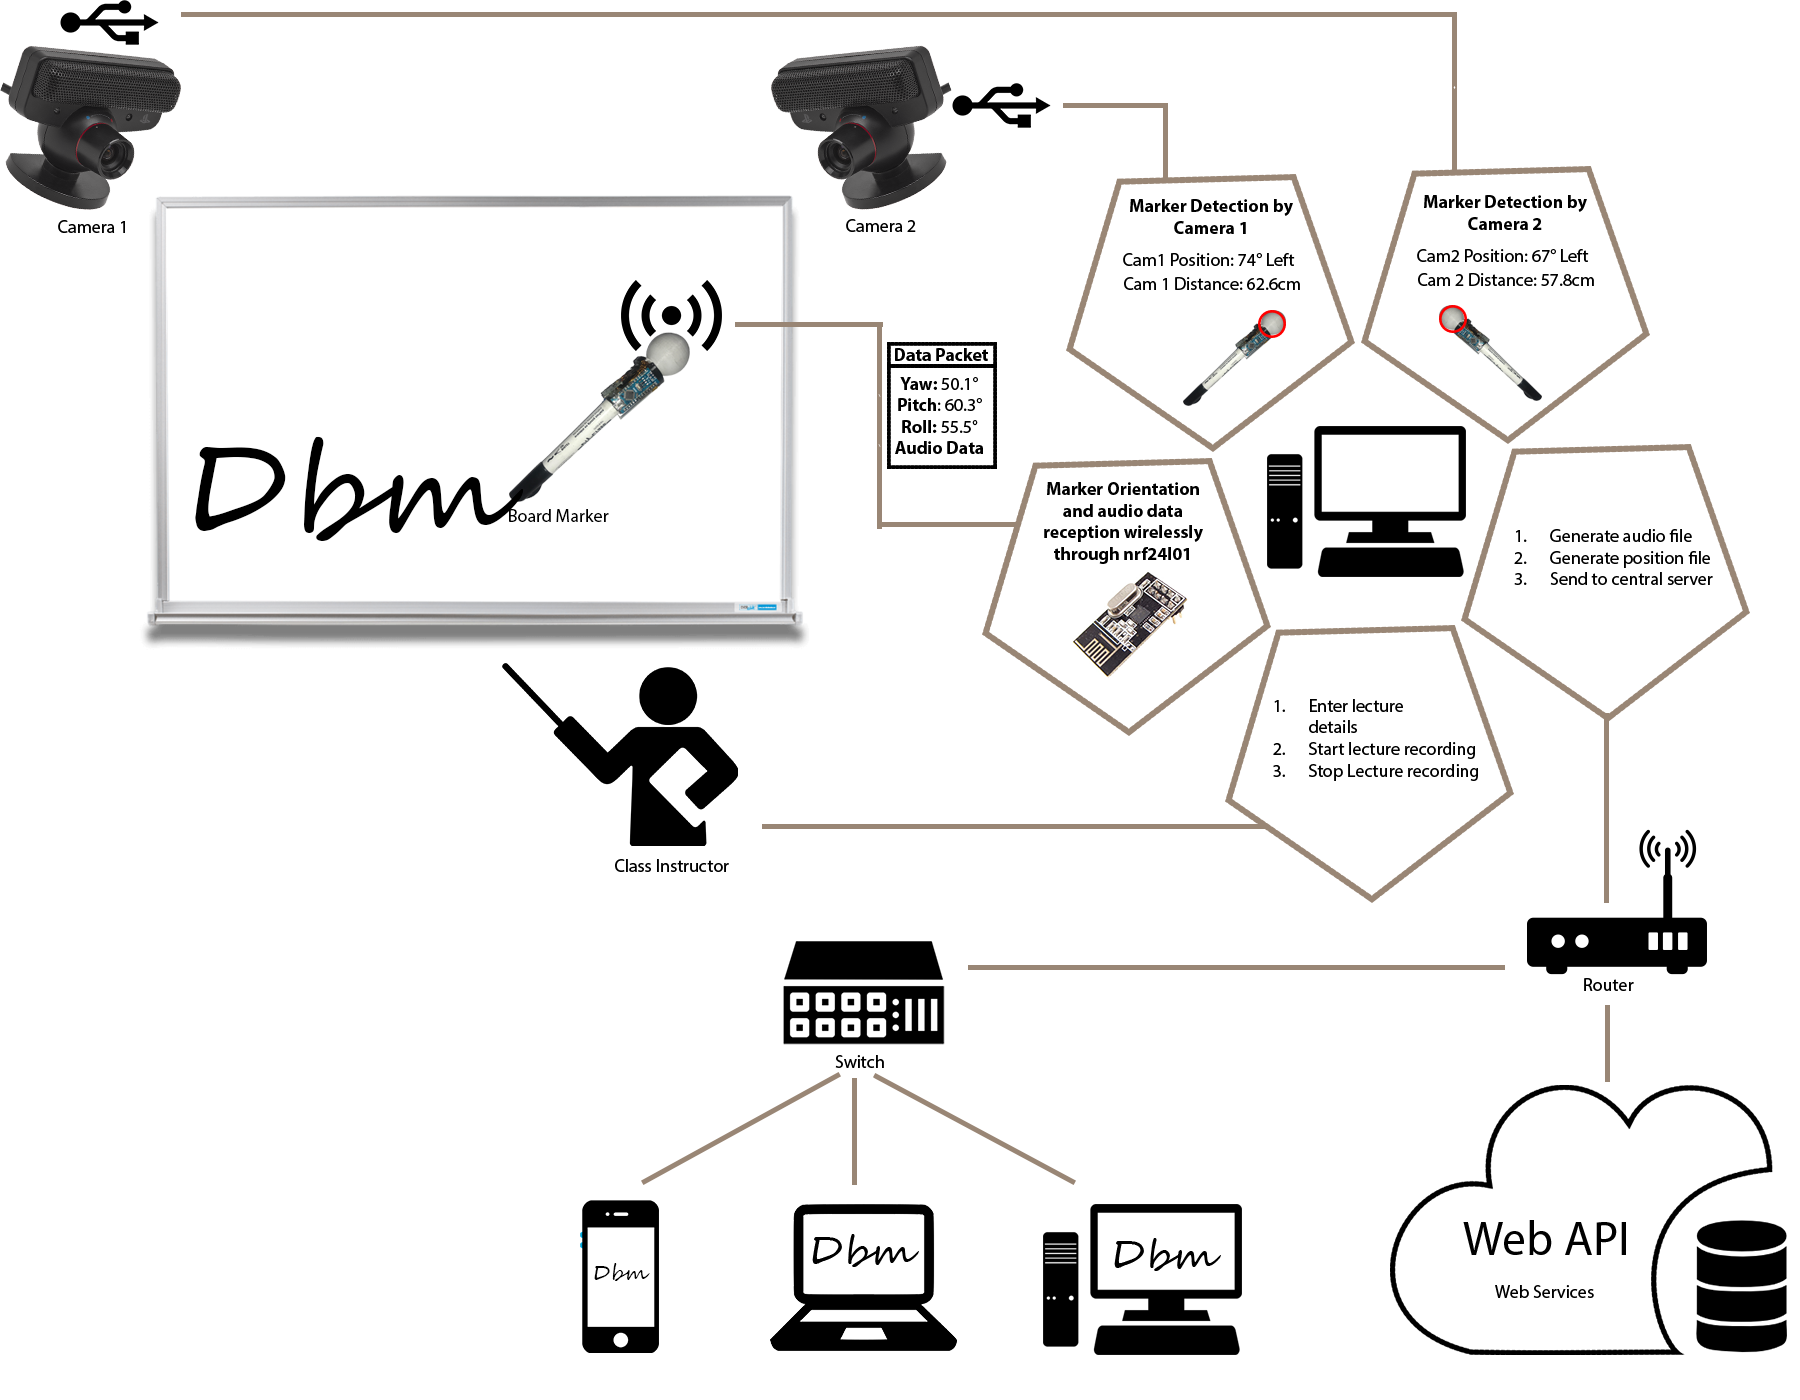
\includegraphics[width=16cm, height=14cm]{Architect 3}
  \caption{Architecture Diagram of Digital Board Marker}
\end{figure}
\bigskip

\section{Modules Methodology Description}
System consists of five major modules. General work flow of each module is detailed using visuals and diagrams.
\subsection{Board Marker}
Board marker transfer the position data of currently written word on the platform i.e. Whiteboard. It is subdivided in two sub-modules
\subsection{Audio Hardware}
Wireless voice transmission is done by this module. Voice data is accepted at transmitter module. This data is converted into digital audio. Digital audio is then transmitted to receiver at another end. Receiver module decode the digital audio into analogue audio. Receiver module is attached to computer through Line-in[2] on which controller application is being executed. Controller application encode the analogue audio into lightweight ogg(file extension) file format. After the audio file generation is successful, audio file is then embedded into lecture file and uploaded to central server.
\subsubsection{Stereo Vision Cameras}
At least two high framerate cameras get the video of back ball and send it to controller application. Stereo vision is important for accurately extracting marker position by placing these cameras at such position so that different angles make same alignment to the writing platform irrespective to size. Square and rectangular boards can be mapped to same parent algorithm with simple to calibrate camera placement guide.

\bigskip

\begin{figure}[h]
  \centering
  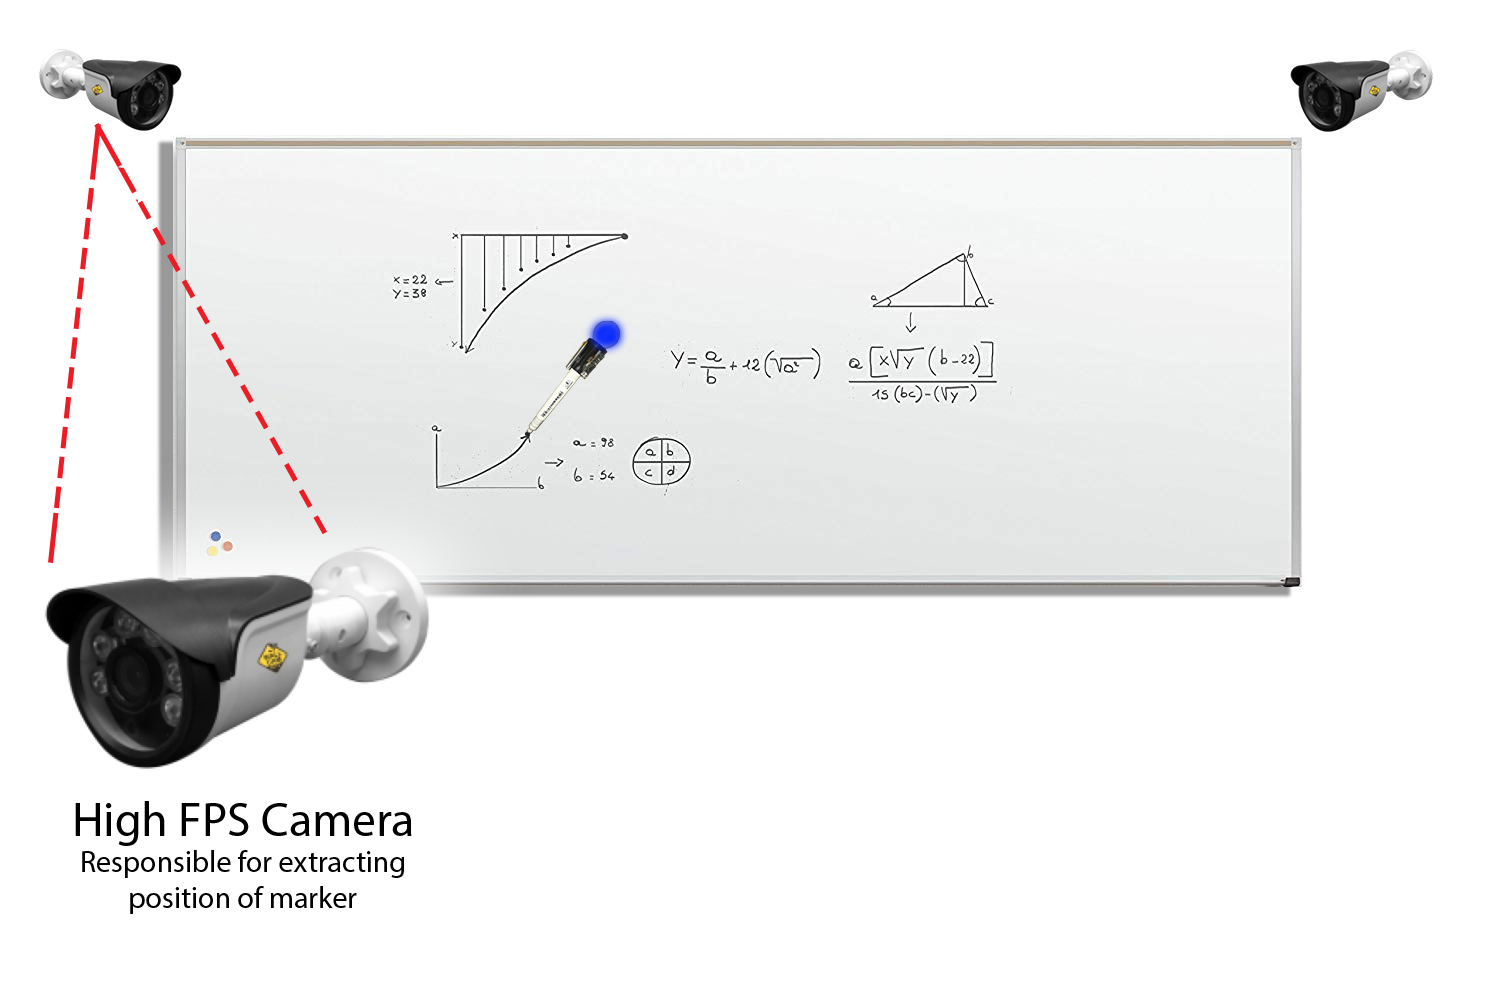
\includegraphics[width=13cm, height=12cm]{Main_Camera}
  \caption{High frame rate camera placement}
\end{figure}





\subsection{Controller Application}
Controller application plays several roles in the project. First of all, it is responsible for application of computer vision algorithms to detect marker and extract the position data. At least two camera perspectives are considered for position extraction. Manual calibration system aids in the setup and view port positioning of multiple cameras. Marker position data and audio data have to be synchronously written in the final output file.\\
Second, it is also responsible for decoding the orientation data. Orientation data is sent using encoded packet by Marker Hardware and received by the controller application. Orientation is extracted using quaternions. Euler angles then extracted using converted quaternion to avoid gimble lock. Position of the marker is extracted.\\
Third, it can play the lecture file before uploading the lecture. Lecture can be paused, resumed and replayed. also, the lecture can be annotated by the instructor i.e. topic and sub-topic markings. Audio and video quality can be controlled over performance of lecture play media.\\

\bigskip
\begin{figure}[h]
  \centering
  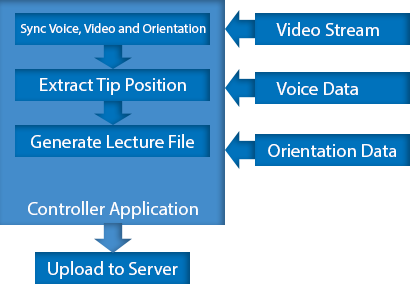
\includegraphics[width=11cm, height=8cm]{Controller Application Methodology}
  \caption{Controller Application General Methodology}
\end{figure}

\subsubsection{Marker Hardware}
To extract marker orientation, Marker Hardware is connected to controller application.

\begin{figure}[h]
  \centering
  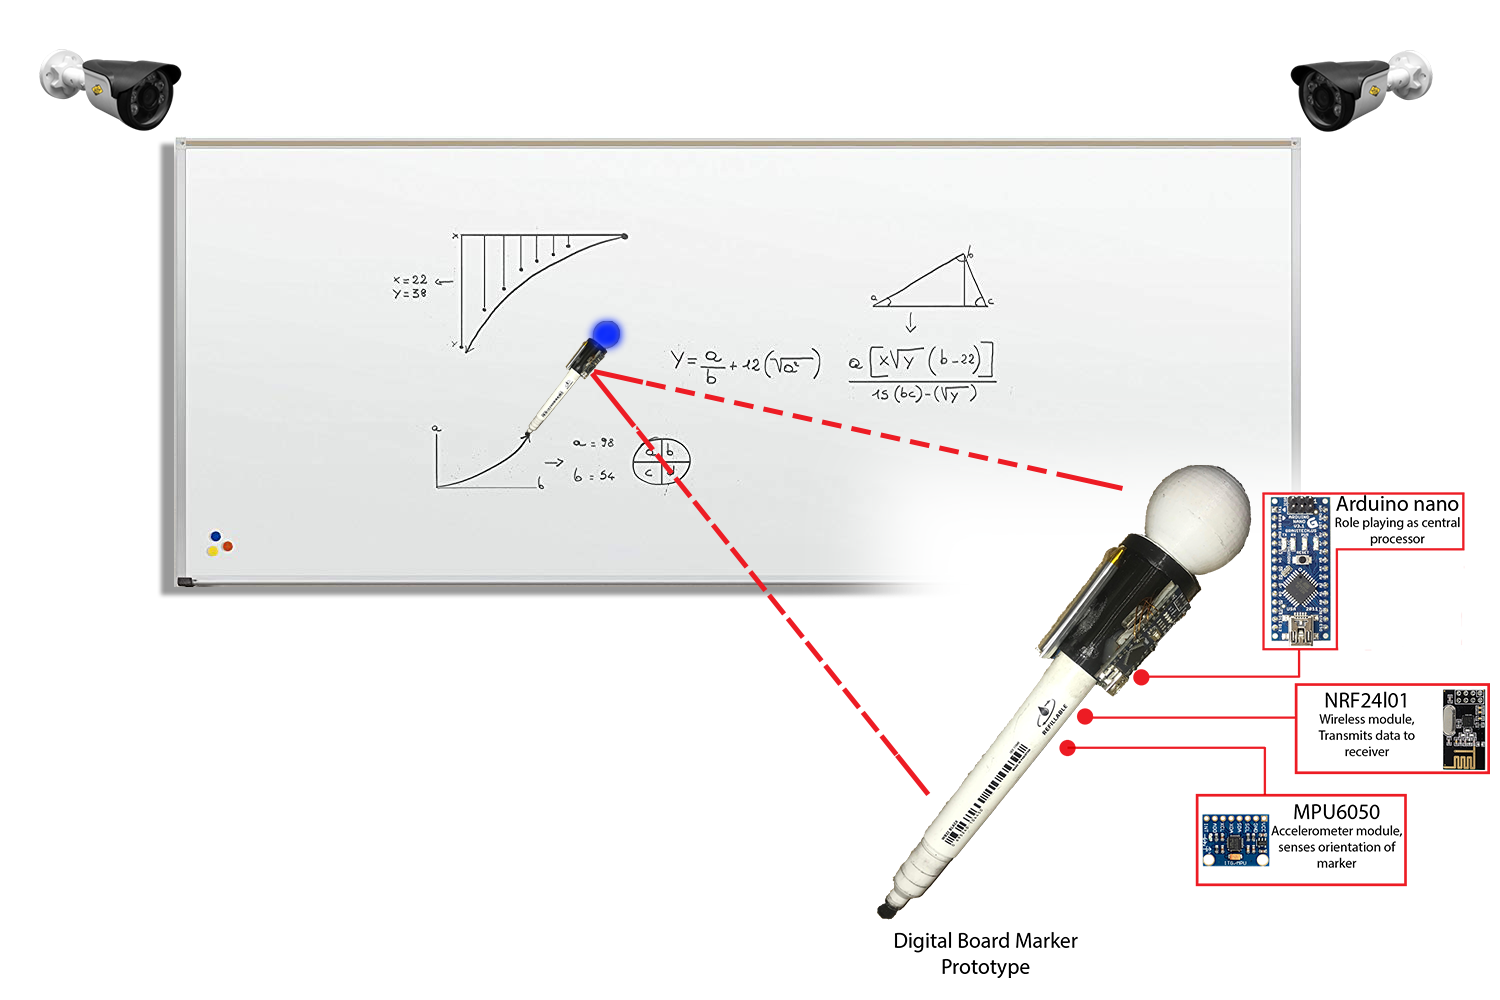
\includegraphics[width=11cm, height=9cm]{Main_Marker}
  \caption{Marker Hardware working methodology}
\end{figure}

\begin{figure}[h]
  \centering
  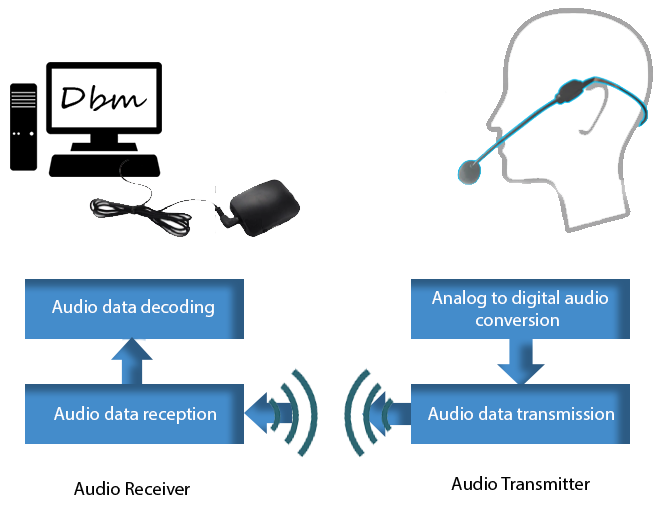
\includegraphics[width=13cm, height=12cm]{Audio Methodology}
  \caption{Audio Hardware General Methodology}
\end{figure}


\subsection{Player Application}
Just like media player, the player application plays the lecture. Common end user of Player Application is student. Player application has two version based on data availability.
\bigskip
\bigskip
\subsection{Offline Player}
Lecture file can be played on the computer via Offline Player with no interaction with internet at all. Typical end user is student. A student can rewind, play, pause, stop and resume while watching the lecture. As the lecture is being played by generated lecture file So, there is no compromise on quality.
\newpage
\begin{figure}[h]
  \centering
  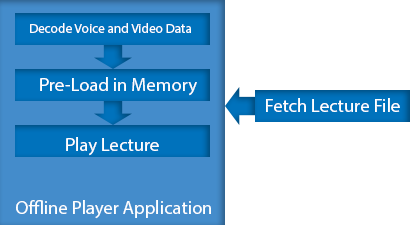
\includegraphics[width=13cm, height=8cm]{Player Application Methodology (Offline)}
  \caption{Offline Player Application General Methodology}
\end{figure}

\subsection{WebGL Player}
It is an online in-browser player that streams the lecture right in the webpage. Similar to video media player, flow of video can be controlled by user. This online player first loads its necessary packages and plugins before it could be fully functional. While browsing the lecture hierarchy, any lecture can be played by user and annotated by an instructor.

\begin{figure}[h]
  \centering
  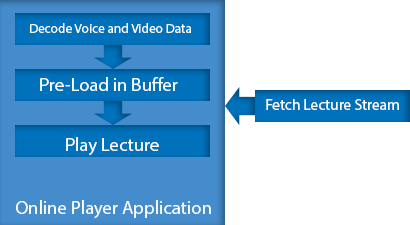
\includegraphics[width=13cm, height=8cm]{Player Application Methodology (Online)}
  \caption{Online Player Application General Methodology}
\end{figure}

\newpage
\subsection{Learning Management System}
LMS System that provides platform for playing online lectures, assignment submission and course content management. This module will act as a final deliverable when integrated with Online Lecture Player. This module consists of many sub-modules and functionalities. It also acts as an online portal for students and play important role in maintaining their profile. Below is further detailed discussion about this module. LMS developed for this project has other features including Administration, Access to high quality study material and learning data, email updates for students as well as teachers, fast delivery of learning material guided by the instructor and organized by existing institute, updates of emerging technologies to make students up-to-date and excel in their career in future. Report generation is another major advantage of the developed module. Using this functionality, instructor of the class can generate reports daily, weekly, monthly and so on. Also, reports are not only about the students. They can be about course material and Lecture data as well. Attendance of students and instructors as well can be maintained and reported easily. Concerned party can view the generated report at any time. Students can view timetable. Concerned instructor can suggest the adjustments to the timetable that administration can see and adjust accordingly. The application is web based so that accessibility of the system could be increased. Reliability and security are major concerns to the system. Administration can suspend the user by analysing the suspicious activity performed by the corresponding person.
\subsubsection{Entity Relationship Diagram}
\begin{figure}[h]
  \centering
  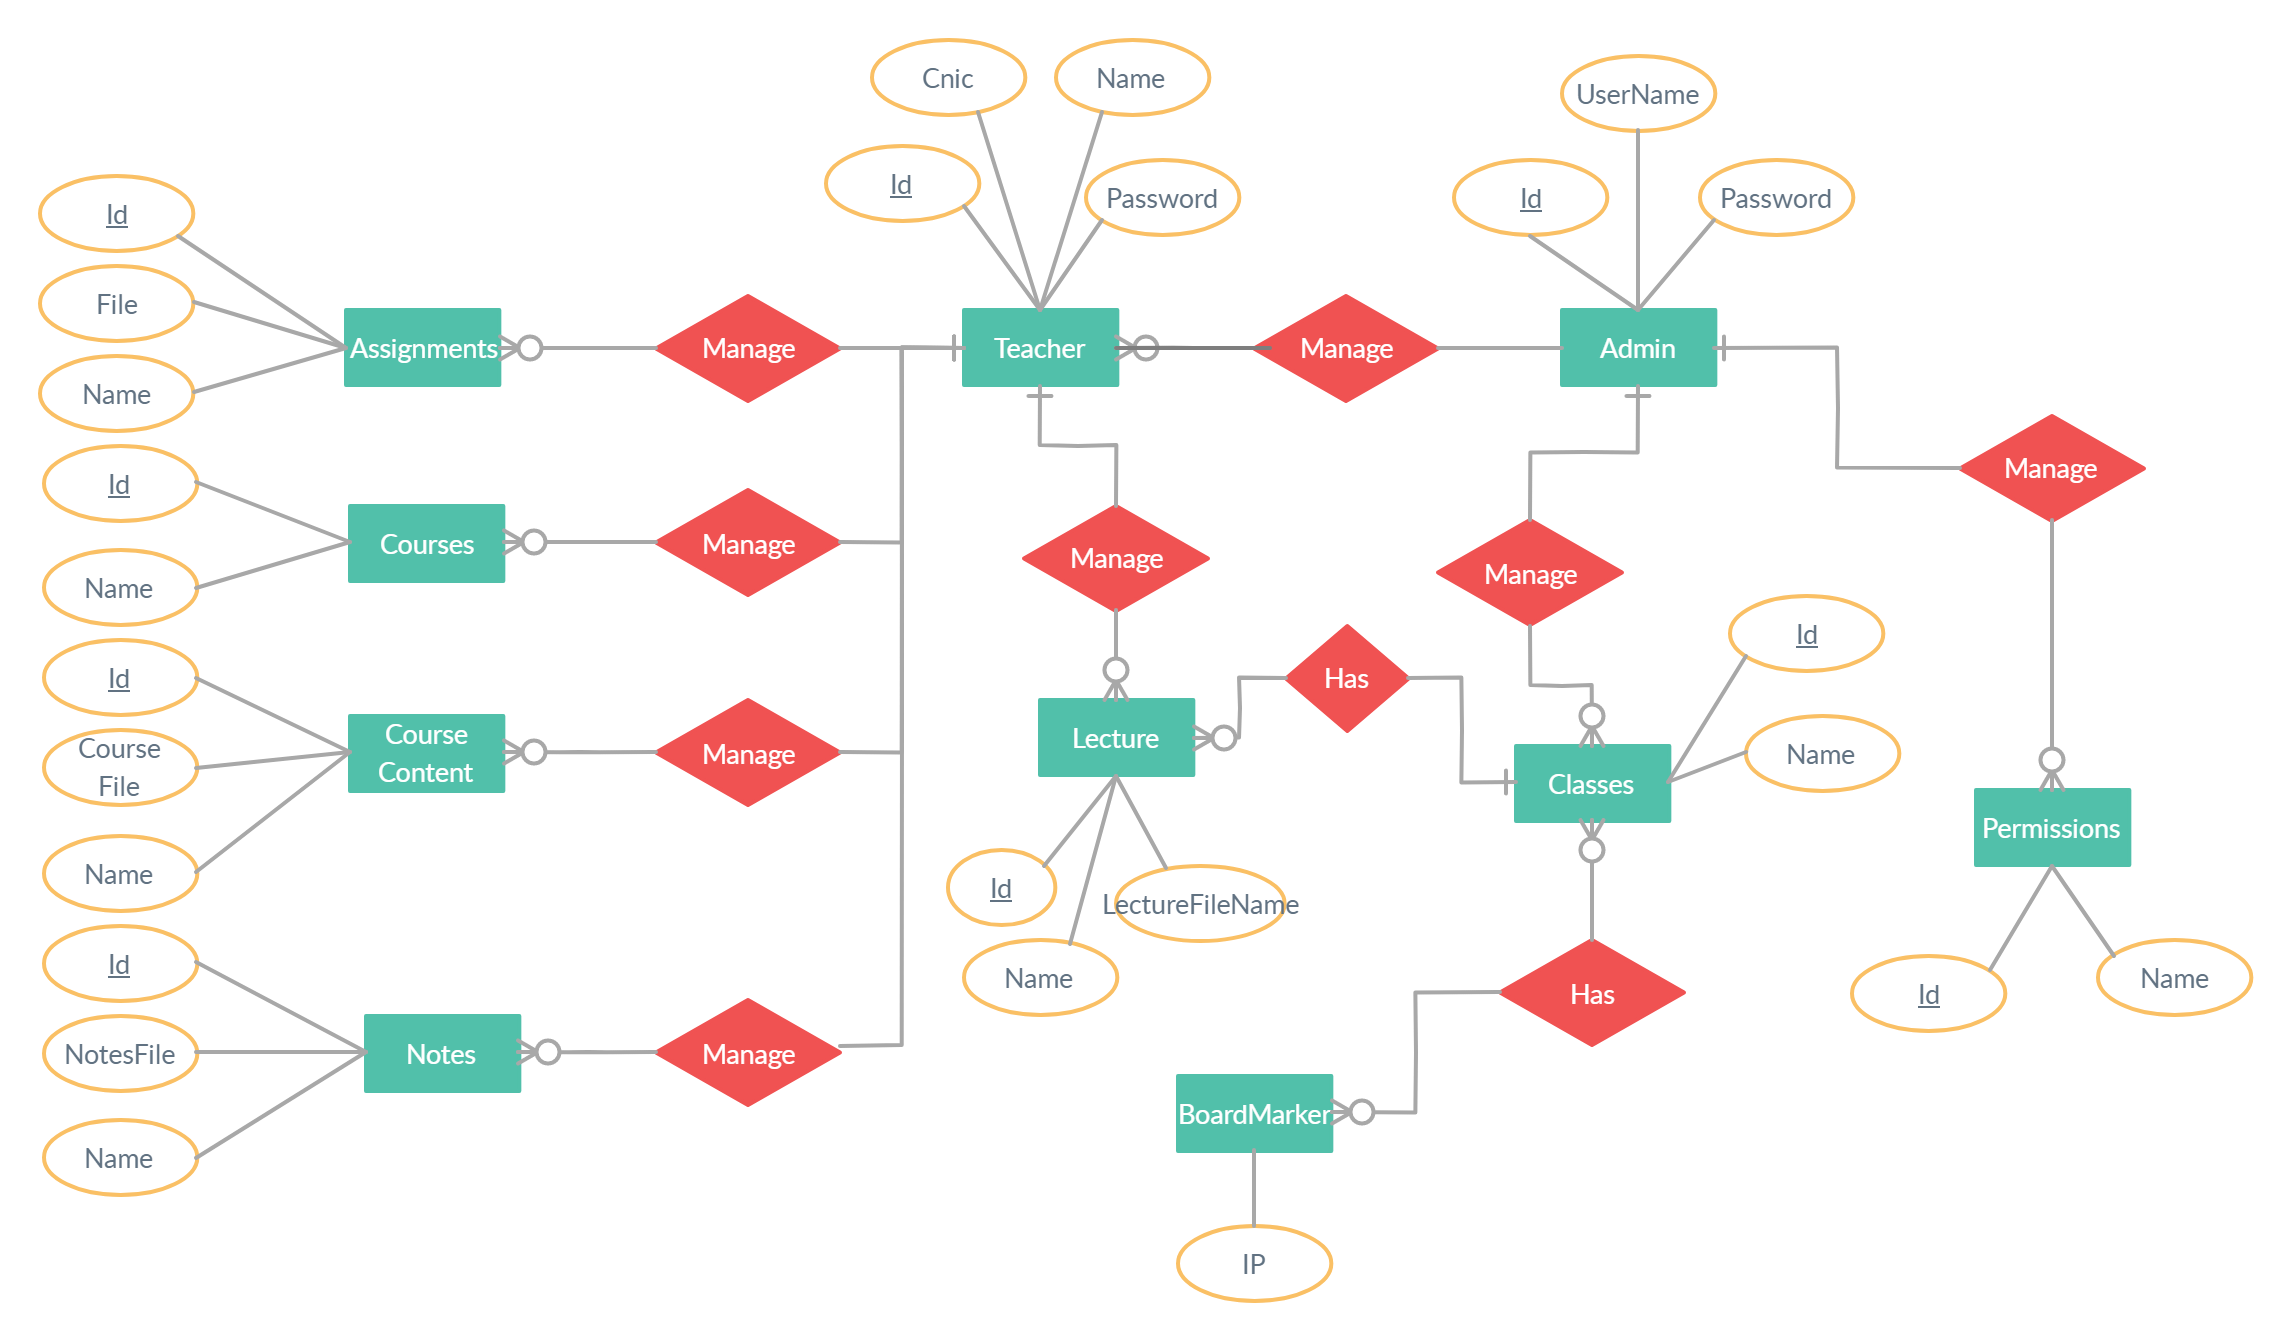
\includegraphics[width=13cm, height=7cm]{Entity Diagram}
  \caption{ER Diagram of LMS}
\end{figure}
\newpage


\subsubsection{Database Diagram}
\begin{figure}[h]
  \centering
  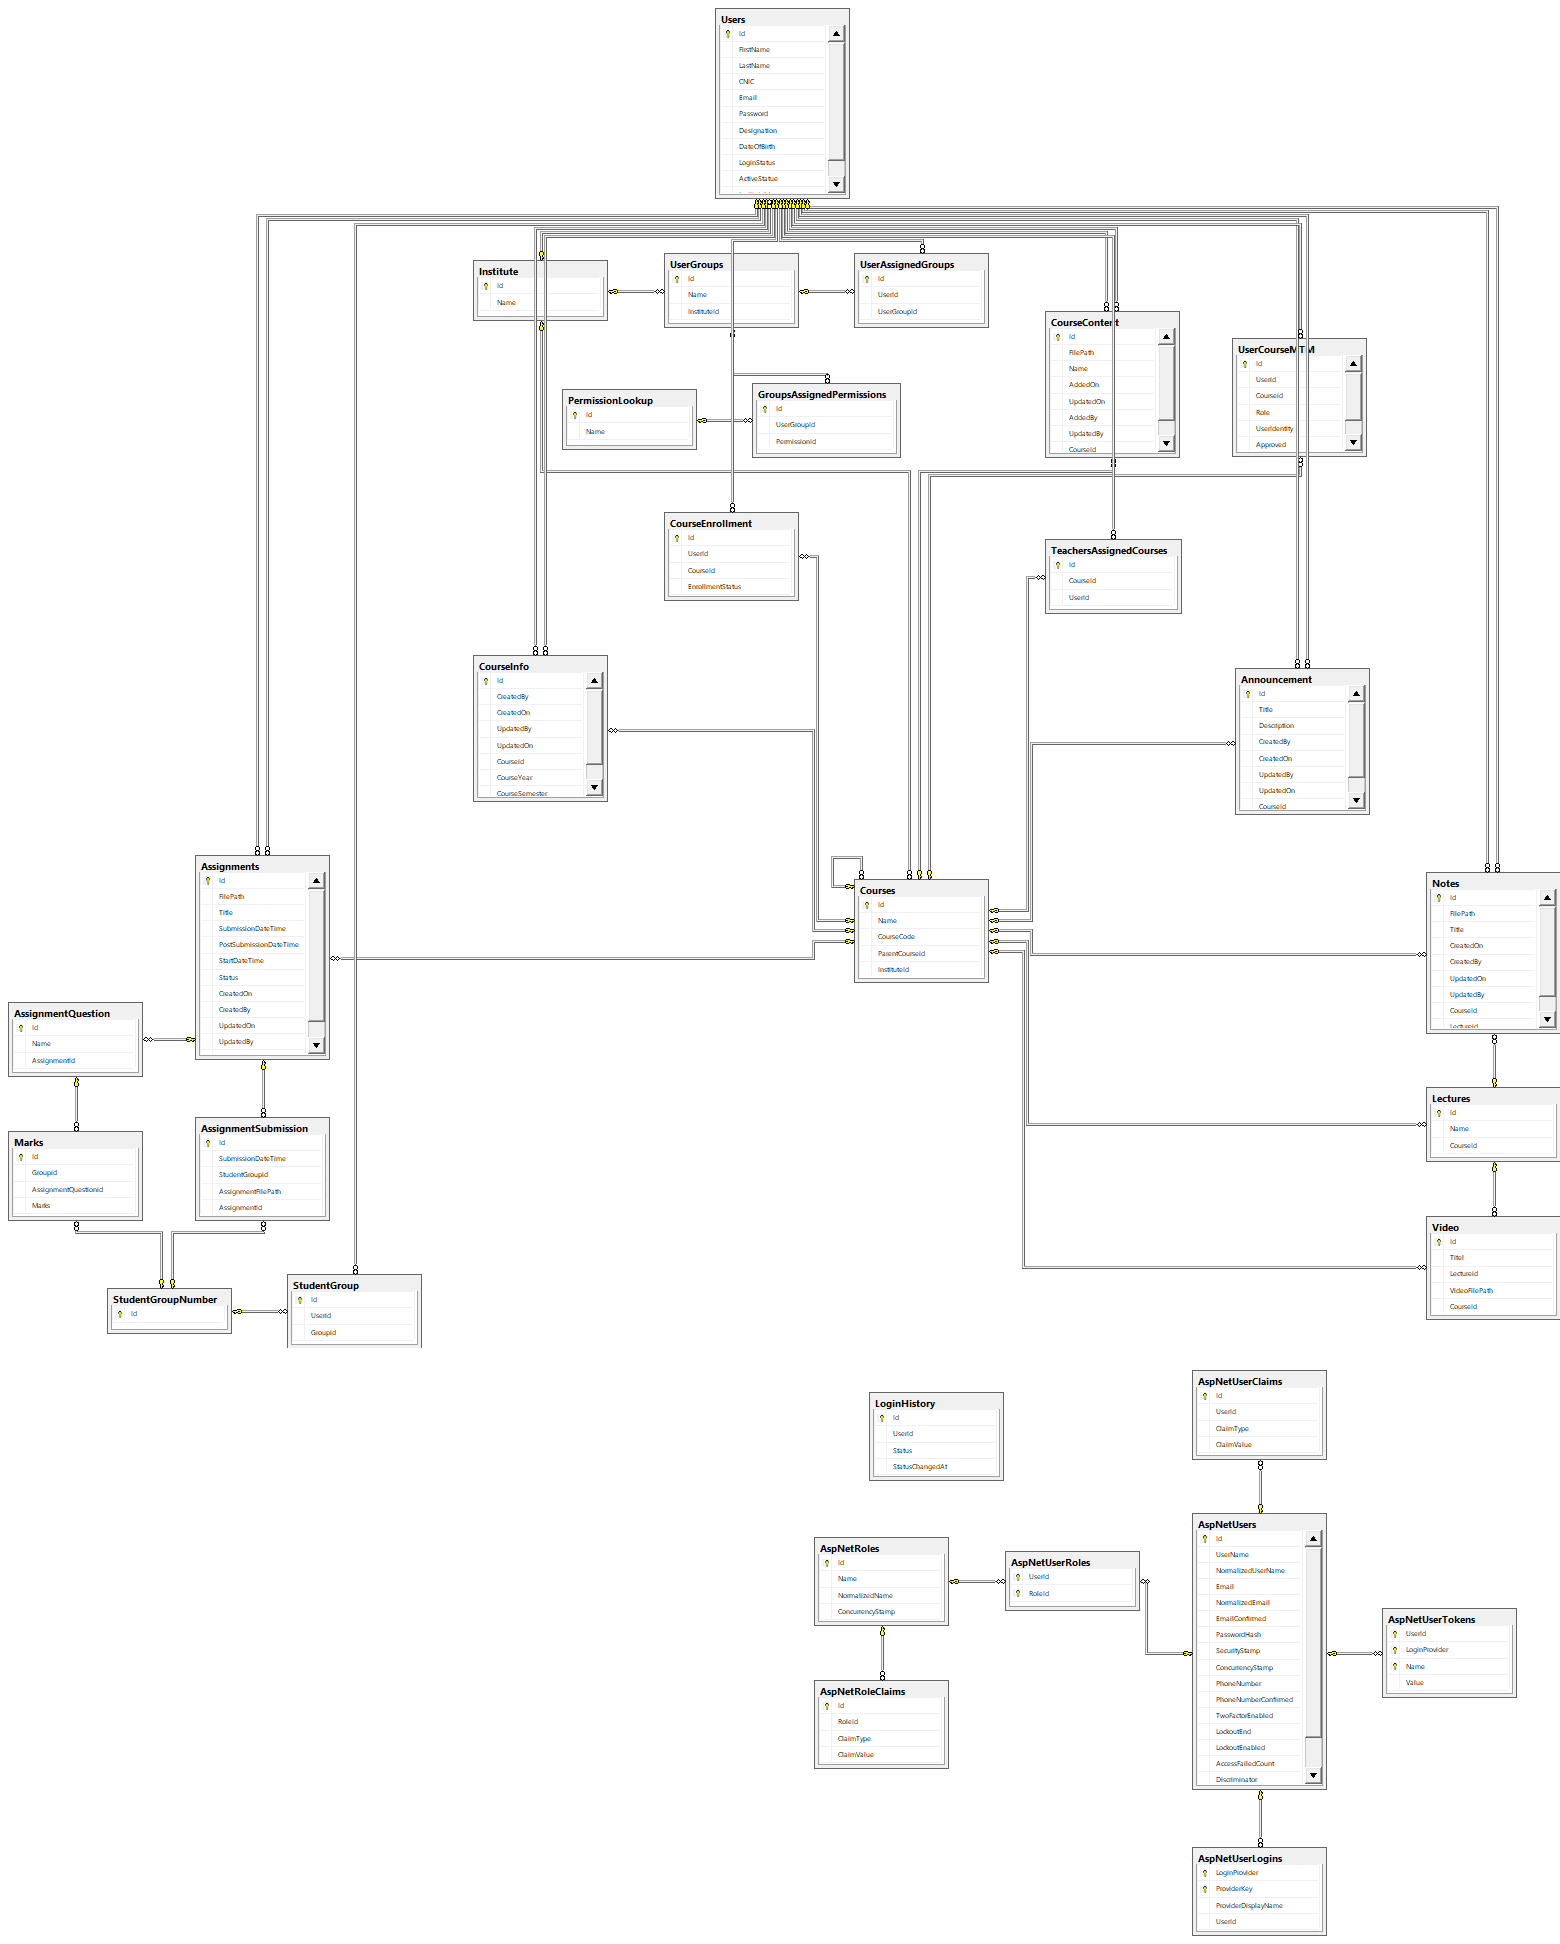
\includegraphics[width=15cm, height=13cm]{DBM_DB_Diagram}
  \caption{DB Diagram of LMS}
\end{figure}

%
%
%
%
%
%%\begin{figure}[h]
%%  \centering
%%  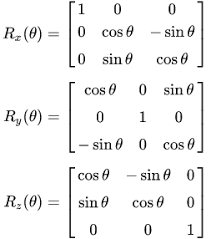
\includegraphics[width=1cm, height=1cm]{EulerAngles}
%%%  \caption{General Flow of the Project}
%%\end{figure}
%
%
%
%
%
%
%
%
%
%
%
%
%
%
%
%
%
%
%
 % Experimental Setup

% Chapter 4

\chapter{Implementation Details} % Write in your own chapter title
\label{Chapter4}
\lhead{Chapter 4. \emph{Implementation Details}} % Write in your own chapter title to set the page header

\section{Implementation}
The system consists of five major modules i.e. Marker Hardware, Audio Hardware, Controller Application, Player Application and LMS Web Application. Implementation detail of each module is discussed below.

%\mbox{}\\

\section{Overall Project Structure}
This diagram shows how the modules are connected and how the effort is implemented to develop modules and connect them to form a Digital Board Marker system.

\mbox{}\\

\begin{figure}[h]
  \centering
  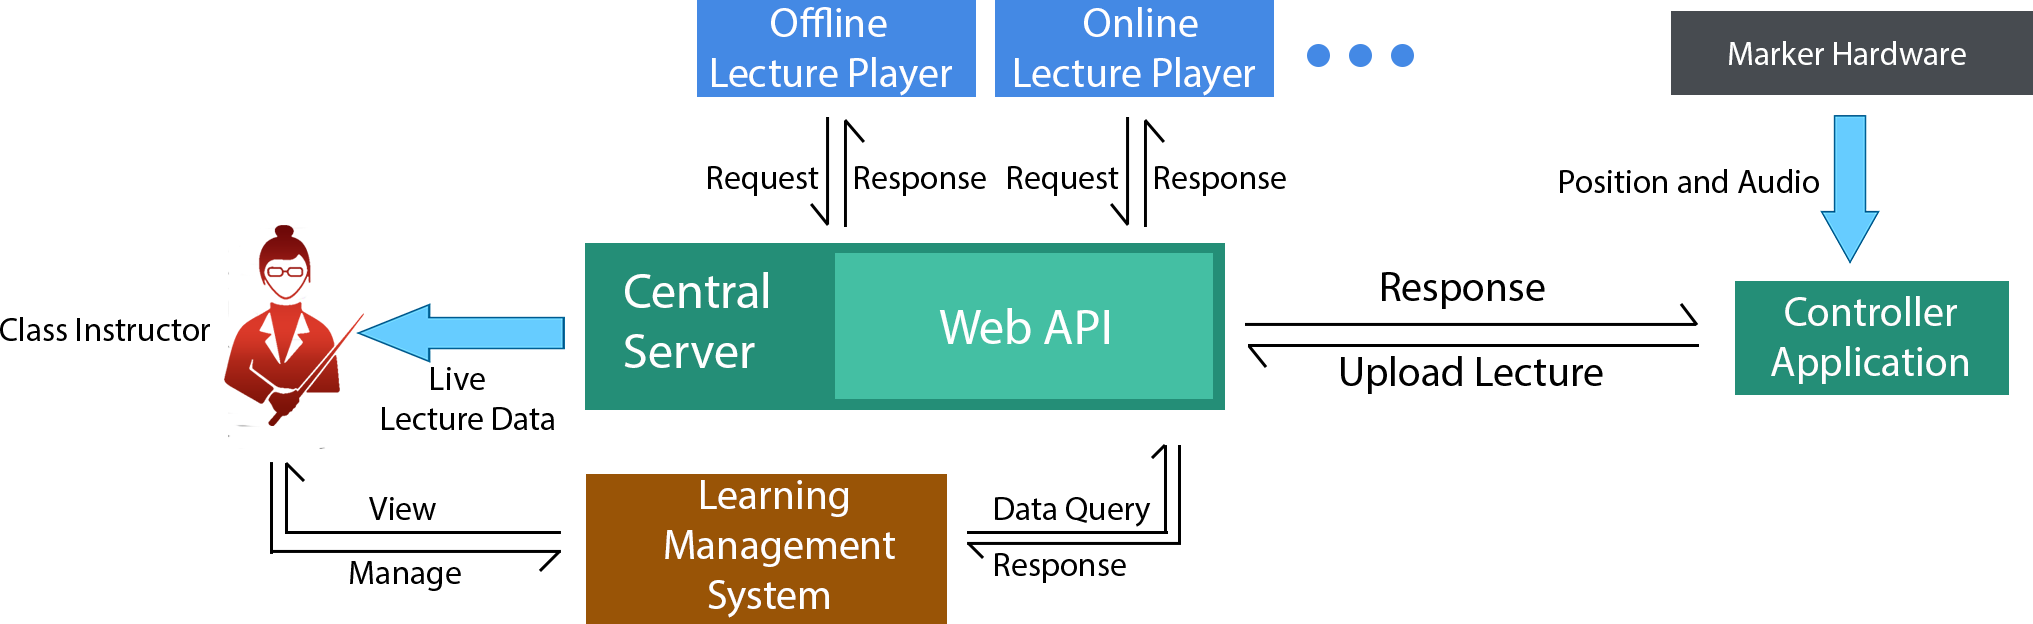
\includegraphics[width=15cm, height=4cm]{Project Structure}
  \caption{Overall Project Structure}
\end{figure}
\newpage
\section{Marker Hardware}
The role of this module is to give orientation and tip pressure of the marker. The module sends data packet that contain encoded orientation of marker in 3d space in form of Euler angles.

\subsection{Requirements Addressed}


\begin{longtable}{|C{1cm}|>{\raggedright\arraybackslash}p{10cm}|C{2cm}|}

\hline


\multicolumn{1}{|>{\centering\arraybackslash}p{1cm}|}{\textbf{\#}} &
\multicolumn{1}{>{\centering\arraybackslash}p{10cm}|}{\textbf{Requirements}}
    & \multicolumn{1}{>{\centering\arraybackslash}p{2cm}|}{\textbf{Priority}}\\
\hline
% Row 1
1 &
Determine orientation of board marker and calculate respective Euler angles &
HIGH \\
\hline

2 &
Transmit the calculated Euler angles to desktop app via nrf24l01 module &
HIGH \\
\hline

3 &
Transmit the calculated Euler angles to desktop app via RS232 serial connection &
LOW \\
\hline

4 &
Turn on using 3.6 volts Li-po battery with Boost converter circuit &
MEDIUM \\
\hline

5 &
Build battery charging circuit within board marker &
LOW \\
\hline

6 &
Implement RGB Led for positioning purpose (Input for camera module) &
HIGH \\
\hline

\caption{Board Marker Hardware Requirements}

\end{longtable}

\subsection{General Flow}
\begin{itemize}

\item Board Marker try to establish wireless connection with the receiver. RGB Led fades meanwhile.
\item RGB Led turns to constant red after successful connection.
\item Accelerometer unit in the Board Marker determines the orientation data.
\item NRF24l01 wireless module in the Board Marker transmits the orientation data to Receiver wirelessly.
\item Receiver Transfers orientation data to desktop app via serial connection.

\end{itemize}

\subsection{Detailed Design}
Marker hardware has two major sub-modules named as \textbf{Transmitter} (marker itself) and \textbf{Receiver}. Below is the detail of components:
\subsubsection{Tact Tactile Switch}
Toggle switch that turns on/off the system when runs on Battery. It does not have any effect when system is running via USB cable.

\begin{figure}[h]
  \centering
  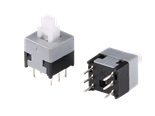
\includegraphics[width=7cm, height=6cm]{Tact Tactile Switch}
  \caption{Tact Tactile Switch}
\end{figure}

\subsubsection{USB DC-DC Boost Converter}
Converts the 3.7V to 5V to turn on and constantly run the Arduino nano prototype board. This sub-module has built-in charging circuit that charges the battery through USB connection.

\begin{figure}[h]
  \centering
  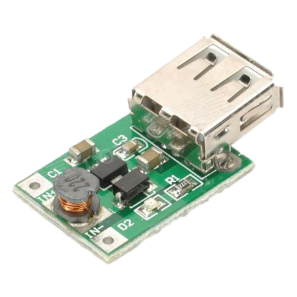
\includegraphics[width=7cm, height=7cm]{DC-DC Boost Converter}
  \caption{DC-DC Boost Converter}
\end{figure}


\subsubsection{Glowing Ball}
Round shaped glowing ball can glow in any combination of RGB colors. It is not for just looks but acts as an input to Stereo cameras for position tracking.

\begin{figure}[h]
  \centering
  
\includegraphics[width=6cm, height=7cm]{Glowing Ball}
  \caption{Glowing Ball}
\end{figure}


\subsubsection{Arduino nano}
Arduino nano acts as main processing board to which all modules and sensors are attached. It acts just like a motherboard with central processor chip soldered on mainboard.

\begin{figure}[h]
  \centering
  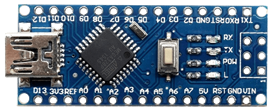
\includegraphics[width=9cm, height=4cm]{Arduino nano}
  \caption{Arduino nano}
\end{figure}


\subsubsection{Li-po battery}
600mAh 3.7V Li-po battery used to run system while there is no USB connection. Voltage may be up to 4.2 volts when fully charged. \\
\underline{DC-DC Boost Converter} is hooked up with the battery that charges the battery as well as raises its voltage to 5V to make the \underline{Board Marker Transmitter} working properly.
\newpage
\begin{figure}[h]
  \centering
  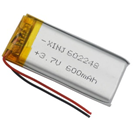
\includegraphics[width=7cm, height=6cm]{Li-po Battery}
  \caption{Li-po Battery}
\end{figure}


\subsubsection{dc-le14112 RGB Led}
3W RGB Led used to create custom color of choice, the corresponding color that is required for position sensing can glow in Glowing ball. It may be given external power source but, in our case, it is directly connected to \underline{Arduino nano}.

\begin{figure}[h]
  \centering
  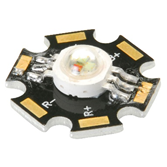
\includegraphics[width=7cm, height=7cm]{RGB Led}
  \caption{RGB Led}
\end{figure}


\subsubsection{MPU-6050}
MPU-6050 or GY-521 board contains accelerometer and gyroscope packed in a single chip. It senses the orientation of the object. It is connected to \underline{Arduino nano} via I2C bus.
\newpage
\begin{figure}[h]
  \centering
  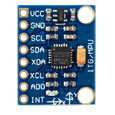
\includegraphics[width=5cm, height=6cm]{MPU-6050}
  \caption{MPU-6050}
\end{figure}


\subsubsection{nRF24L01}
nRF24L01 is a single chip radio transceiver. It is responsible for transmitting orientation data from transmitter module to receiver.

\begin{figure}[h]
  \centering
  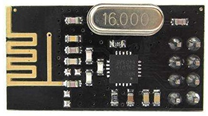
\includegraphics[width=8cm, height=4cm]{nRF24L01}
  \caption{nRF24L01}
\end{figure}

\subsection{Marker Transmitter}
The objective of the transmitter module is to extract orientation of the board marker. The challenge is the marker is changing its orientation while writing on the board. Transmitter module is designed as a back cap of board marker. It is attached to the board marker to record orientation of marker. The role of this sub-module is to transmit the tip pressure and orientation of marker in space. Further details of each part constituting the transmitter are given below.

\subsubsection{Components Used}
Detailed description of electronic components excluding discrete consumer parts, e.g. wires, is given below and described above.
\newpage
\begin{figure}[h]
  \centering
  \includegraphics[width=7cm, height=9cm]{Marker Parts}
  \caption{Board Marker with Transmitter Components}
\end{figure}

\subsubsection{Component Connection Diagram}
This diagram represents how sub-modules or components are connected in Transmitter module.
\begin{figure}[h]
  \centering
  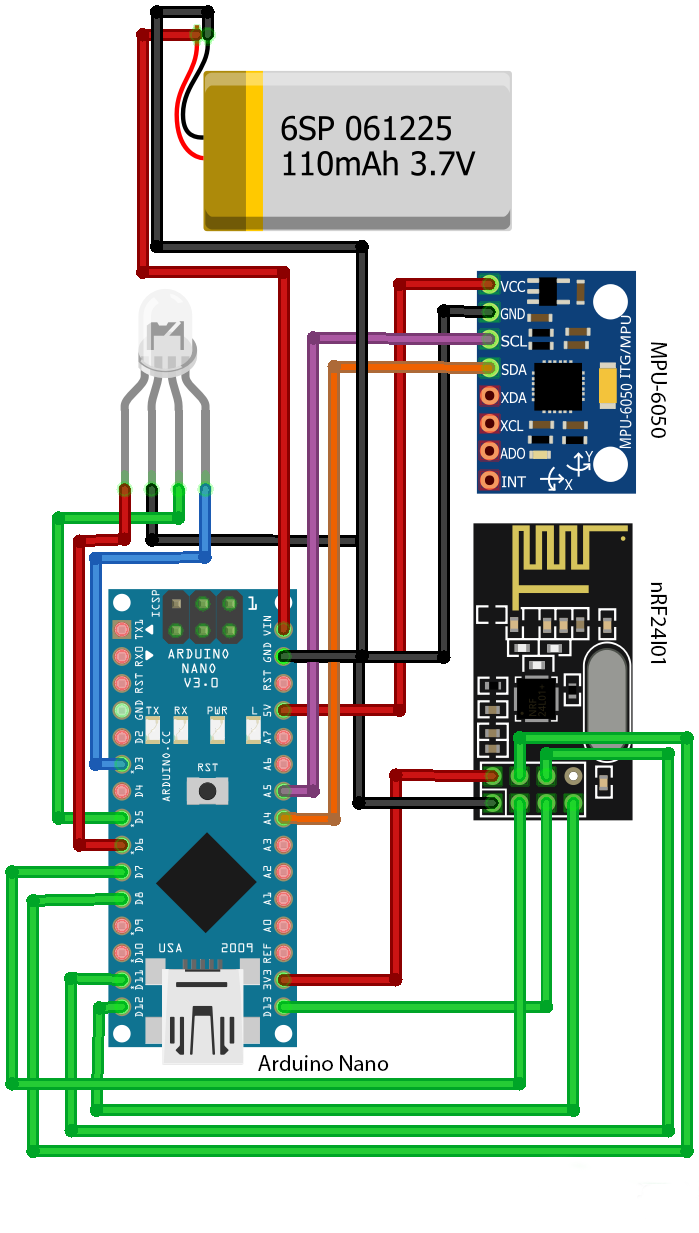
\includegraphics[width=6cm, height=9cm]{Marker Transmitter_bb}
  \caption{Component connection diagram of Board Marker Transmitter}
\end{figure}

\subsubsection{Schematic Diagram}
Schematic diagram of Board Marker Transmitter can be seen as below

\begin{figure}[h]
  \centering
  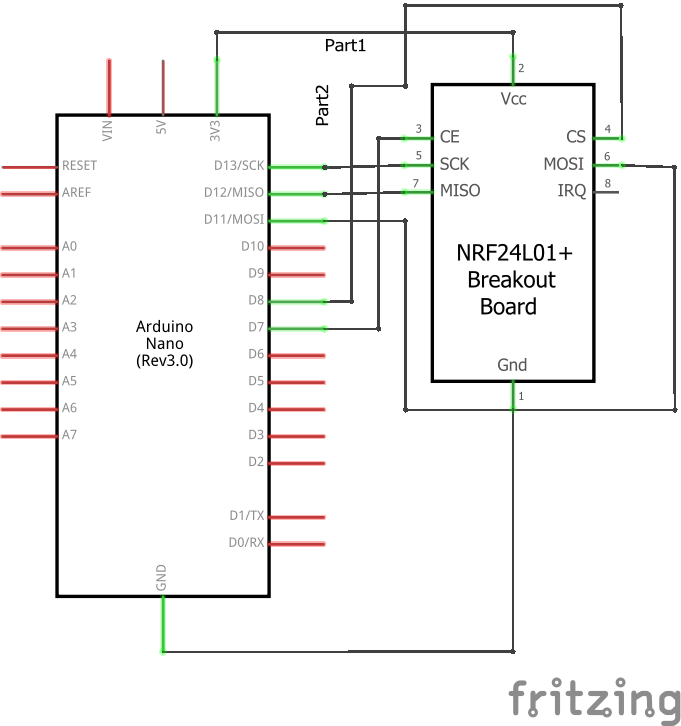
\includegraphics[width=6cm, height=8cm]{Marker Receiver_schem}
  \caption{Schematic diagram of Board Marker Transmitter}
\end{figure}


\subsubsection{General Flow}

\begin{figure}[h]
  \centering
  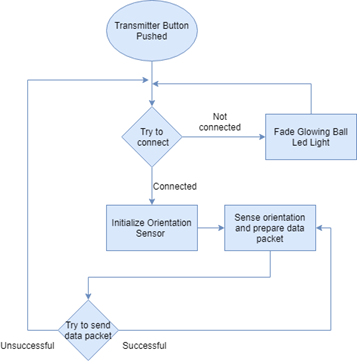
\includegraphics[width=9cm, height=10cm]{Marker Transmitter}
  \caption{General Flow of Board Marker Transmitter}
\end{figure}


\subsection{Marker Receiver}
Receiver module receives orientation data as Euler angles and transfer it to the desktop application via USB connection. As it is connected via USB so it does not need any external power source.

\subsubsection{Component Connection Diagram}

\begin{figure}[h]
  \centering
  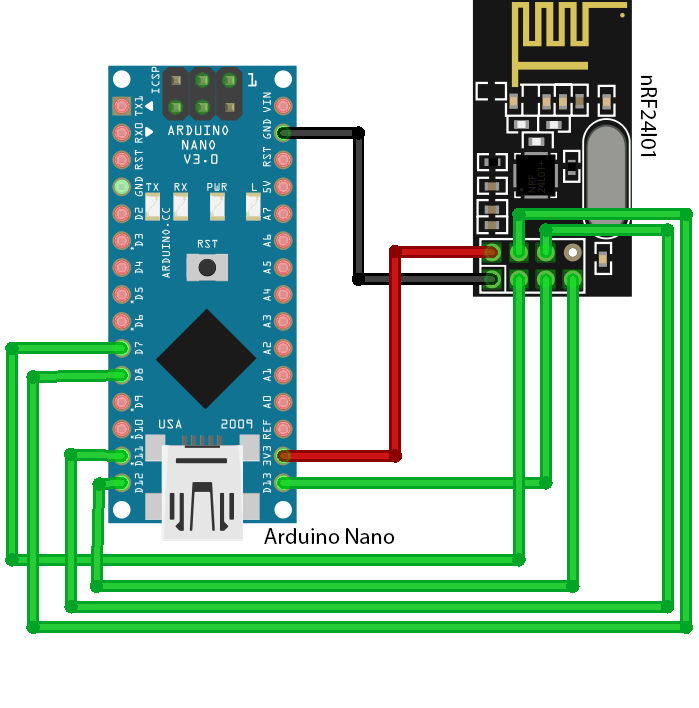
\includegraphics[width=5cm, height=6cm]{Marker Receiver_bb}
  \caption{Component connection diagram of Board Marker Receiver}
\end{figure}

\subsubsection{Schematic Diagram}
Schematic diagram that shows abstract component view of Receiver module is given below

\begin{figure}[h]
  \centering
  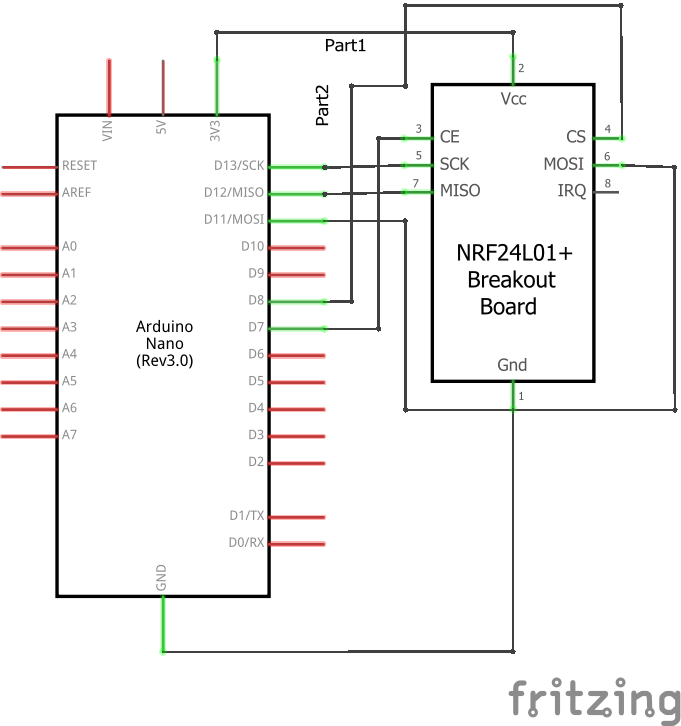
\includegraphics[width=5cm, height=7cm]{Marker Receiver_schem}
  \caption{Schematic diagram of Board Marker Receiver}
\end{figure}
\newpage
\subsubsection{General Flow}
\begin{figure}[h]
  \centering
  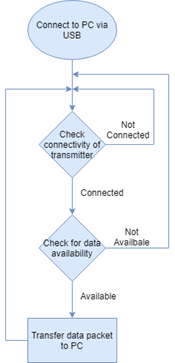
\includegraphics[width=5cm, height=9cm]{Marker Receiver}
  \caption{General Flow of Board Marker Receiver}
\end{figure}

\subsection{Rules and Assumptions}
Following are rules and cases of assumptions that are assumed to be true while normal working
\begin{itemize}

\item Board Marker Transmitter and Receiver are in range of 2 meters for less noise and preventing latency issues.
\item Pressure threshold of board marker tip is 5Pascals that is equivalent to pressure of lead pencil tip. Above this pressure, marker will write and otherwise not.
\item Glowing ball of board marker must be at least partially visible by either of the cameras. Precision of marker position decreases from Case 1 to 6. Best Accuracy in Case 1 and no output at all in Case 6.
\item User is supposed to be not touching the Marker tip while recording the lecture.
\item User is supposed to be write only in the boundary of the defined platform i.e. whiteboard. 

\end{itemize}
\newpage
\begin{figure}[h]
  \centering
  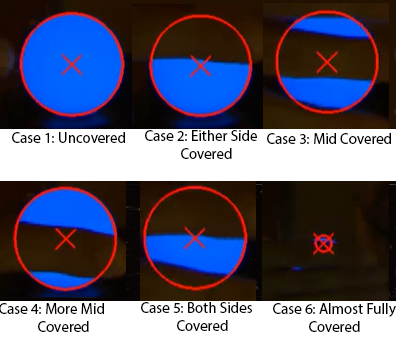
\includegraphics[width=9cm, height=8cm]{Ball cover}
  \caption{Glowing Ball Detection While Covered}
\end{figure}

\subsection{Tools and Technologies used}
List all software that are used to develop and needed to operate the developed module are detailed below.

\subsubsection{Arduino IDE v1.8.9}
Code environment in which all code for Board Maker Transmitter and Receiver is written. This IDE is numerously used as a debugging tool as well.

\subsubsection{Processing v3.5.3}
This tool is used for debugging and visualization of Board Marker Transmitter as a teapot object. In order to view Board Marker Transmitter and verify the placement of MPU-6050 orientation sensor and latency, we visualized the teapot object moving in the window of Processing software. Following parameters and properties are visualized and debugged.

\begin{itemize}

\item Correct orientation data packet format of Board Marker Transmitter.
\item Generation of noise with respect to obstacles and distance involved while data transmission.
\item Latency in data transmission with respect to obstacles and distance involved while data transmission.

\end{itemize}

Sample image of object is given below
\newpage
\begin{figure}[h]
  \centering
  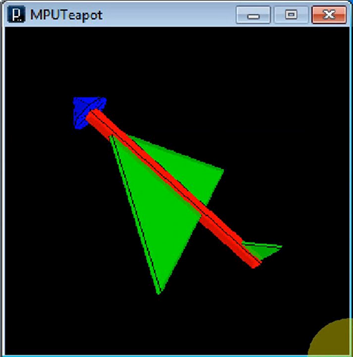
\includegraphics[width=11cm, height=10cm]{Teapot}
  \caption{Marker Orientation Image in Processing Software}
\end{figure}

\section{Audio Hardware}
Role of Audio Hardware is to establish a wireless voice communication between Teacher and Controller Application. The module wirelessly transmits the voice of Teacher to controller app. The module works on 2.4G frequency band approved and approved by RoHS.

\subsection{Requirements Addressed}
\begin{longtable}{|C{1cm}|>{\raggedright\arraybackslash}p{10cm}|C{2cm}|}

\hline


\multicolumn{1}{|>{\centering\arraybackslash}p{1cm}|}{\textbf{\#}} &
\multicolumn{1}{>{\centering\arraybackslash}p{10cm}|}{\textbf{Requirements}}
    & \multicolumn{1}{>{\centering\arraybackslash}p{2cm}|}{\textbf{Priority}}\\
\hline
% Row 1
1 &
Transfer Voice data from one point to another. &
HIGH \\
\hline

2 &
Transfer Voice data from transmitter to receiver wirelessly.  &
HIGH \\
\hline

3 &
Transmitter should be standalone in terms of power. &
HIGH \\
\hline

4 &
Receiver should output voice data as analogue audio wave. &
MEDIUM \\
\hline

5 &
Implement noise control knob in transmitter. &
MEDIUM \\
\hline


\caption{Audio Hardware Requirements}

\end{longtable}

\subsection{General Flow}

\begin{itemize}

\item Transmitter try to connect to the Receiver
\item After a successful connection, Transmitter reads analogue signal and converts it into digital PWM wave.
\item Transmitter then starts transmitting the voice data through nRF24L01 module.
\item Voice data arrives at nRF24L01 of Receiver.
\item Receiver converts the incoming signal into audio wave.


\end{itemize}

\subsection{Detailed Design}
Audio hardware has two major sub-modules named as Transmitter and Receiver

\subsubsection{Electret Microphone}
9767 Condenser Electret Microphone used to capture voice.
\begin{figure}[h]
  \centering
  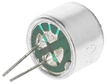
\includegraphics[width=4cm, height=4cm]{Mic}
  \caption{Electret Microphone}
\end{figure}


\subsubsection{100K Resistor}
Used to adjust input gain of microphone. It is connected with the \underline{Microphone Circuit}.

\begin{figure}[h]
  \centering
  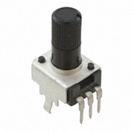
\includegraphics[width=5cm, height=4cm]{Pot}
  \caption{100K Resistor}
\end{figure}

\subsubsection{Microphone Circuit}
An electric circuit implemented on a dotted Veroboard. It transfers the voltage change due to microphone to the \underline{Arduino nano} mainboard


\subsubsection{Input Audio Socket}
3.5mm Audio Socket that is used to input the audio wave. It acts as mono input audio channel.

\subsubsection{Output Audio Socket}
3.5mm Audio Socket that is used to output the audio wave. It acts as mono output audio channel.

\begin{figure}[h]
  \centering
  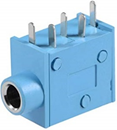
\includegraphics[width=5cm, height=6cm]{3.5mm jack}
  \caption{Audio Jack}
\end{figure}

\subsubsection{Arduino nano}
Arduino nano acts as main processing board to which all modules and sensors are attached. It acts just like a motherboard with central processor chip soldered on mainboard.

\begin{figure}[h]
  \centering
  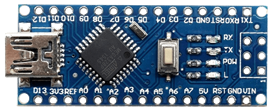
\includegraphics[width=6cm, height=3cm]{Arduino nano}
  \caption{Arduino nano}
\end{figure}

\subsubsection{nRF24L01 Adapter}
5V to 3.3V nRF24L01 adapter gives constant 3.3V from input 5V. It prevents nRF24L01 module not to drain power from \underline{Arduino nano} mainboard.


\begin{figure}[h]
  \centering
  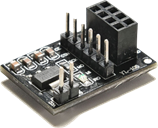
\includegraphics[width=8cm, height=6cm]{nrf Adapter}
  \caption{nRF24L01 Adapter}
\end{figure}

\subsubsection{Noise Reduction Circuit}
The circuit is used to reduce random noise with the help of gradual grounding the input audio wave.


\subsubsection{nRF24L01}
nRF24L01 is a single chip radio transceiver. It is responsible for transmitting voice data from transmitter module to receiver.

\begin{figure}[h]
  \centering
  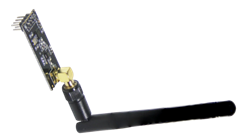
\includegraphics[width=8cm, height=6cm]{nrf Antenna Version}
  \caption{nRF24L01 Antenna Version}
\end{figure}

\subsection{Audio Transmitter}
The objective of the Audio Transmitter is to get voice data from microphone and transmit it to the Audio Receiver. After getting the data from microphone, it converts analogue audio data into a digital Pulse Width Modulation or PWM wave.

\subsection{Components Used}
Detailed description of electronic components excluding discrete consumer parts, e.g. wires, is given below and described above.

\begin{figure}[h]
  \centering
  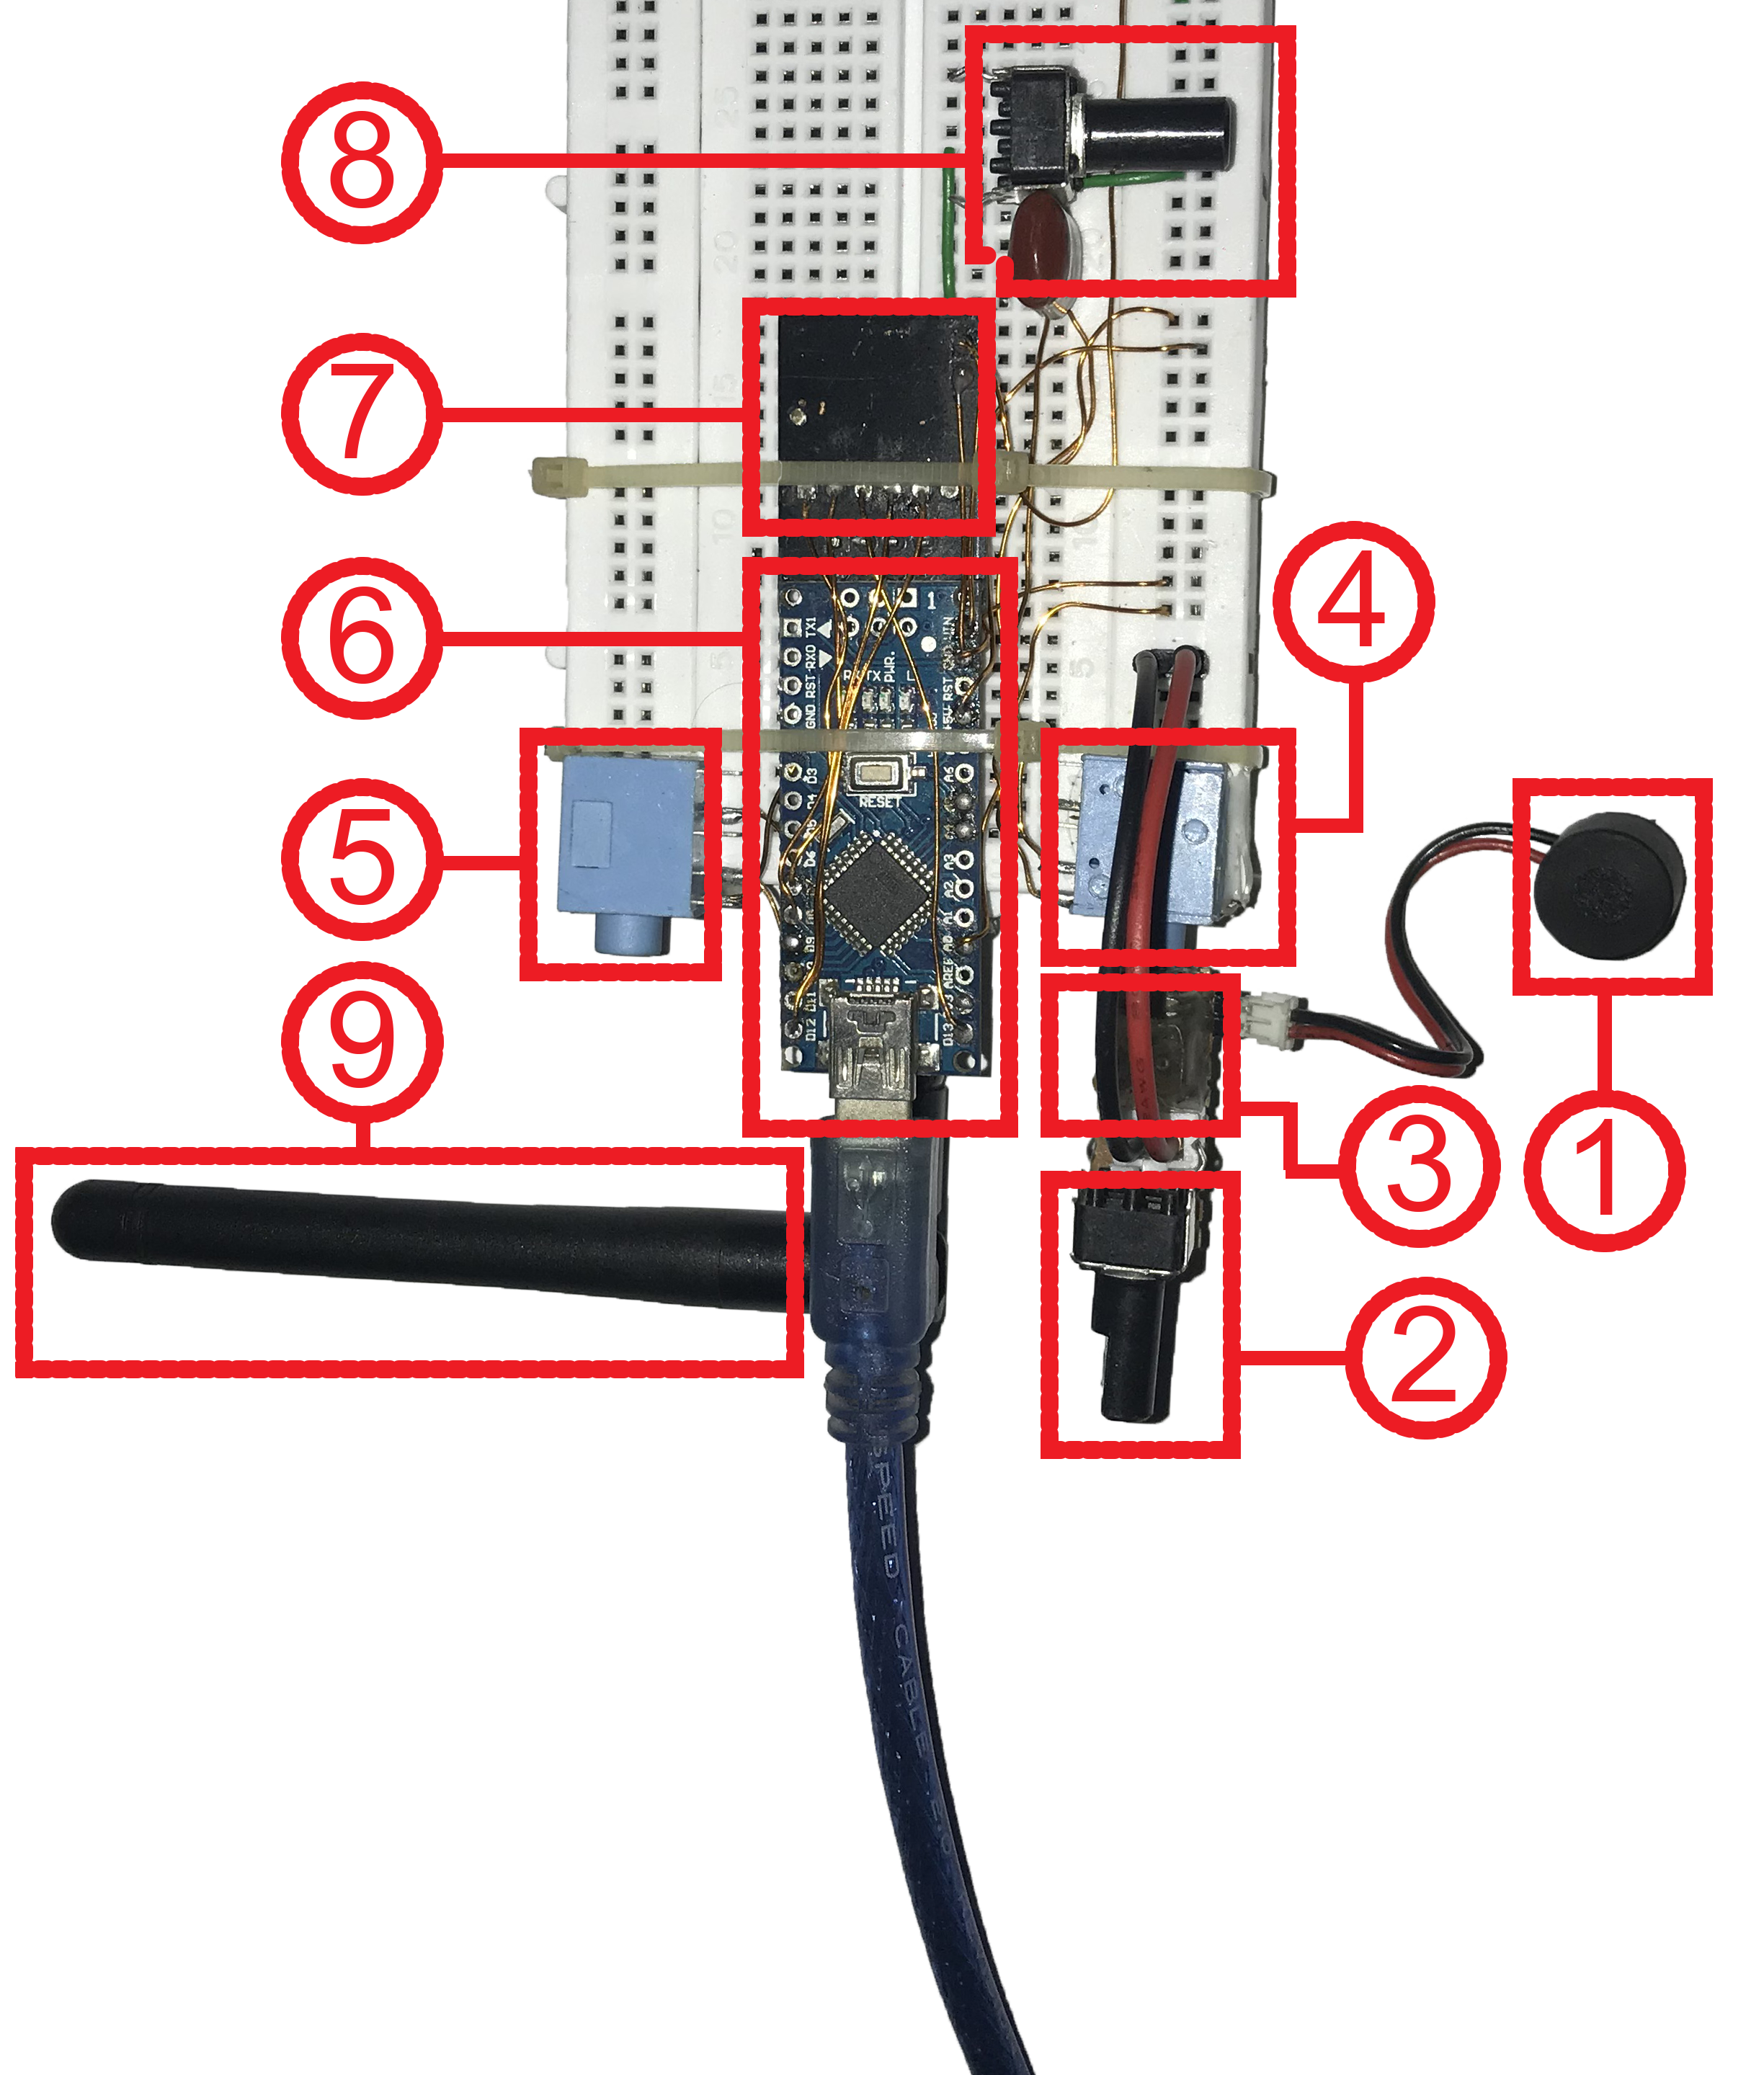
\includegraphics[width=6cm, height=8cm]{Audio Trans num}
  \caption{nRF24L01 Audio Transceiver Component Detail}
\end{figure}

\subsection{Component Connection Diagram}
This diagram represents how sub-modules or components are connected in Transceiver module.


\begin{figure}[h]
  \centering
  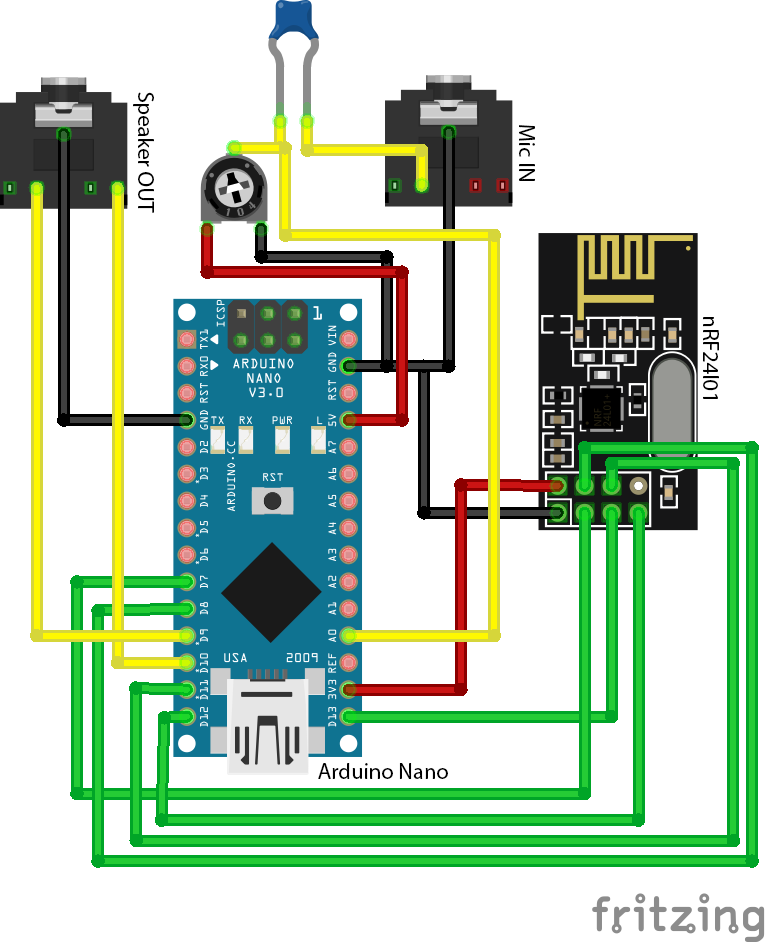
\includegraphics[width=5cm, height=7cm]{Audio Receiver_bb}
  \caption{Audio Transceiver Component Connection Diagram}
\end{figure}


\subsection{Schematic Diagram}

\begin{figure}[h]
  \centering
  \includegraphics[width=7cm, height=8cm]{Audio Receiver_schem}
  \caption{Audio Transceiver Schematic Diagram}
\end{figure}


\subsection{General Flow}

\begin{figure}[h]
  \centering
  \includegraphics[width=8cm, height=9cm]{Audion transmitter flow}
  \caption{General Flow of Audio Transmitter}
\end{figure}

\subsection{Audio Receiver}
Receiver module receives audio data from transmitter. Although the Arduino nano mainboard is programmed differently but the circuit and composition of receiver module is identical to transmitter module.

\subsection{Components Used}
Detailed description of electronic components excluding discrete consumer parts, e.g. wires, is given below and described above.

\begin{figure}[h]
  \centering
  \includegraphics[width=6cm, height=7cm]{Audio Recv num}
  \caption{Component Diagram of Audio Receiver}
\end{figure}

\subsection{General Flow}

\begin{figure}[h]
  \centering
  \includegraphics[width=5cm, height=7cm]{Audion Reciever flow}
  \caption{General Flow of Audio Receiver}
\end{figure}


\subsection{Rules and Assumptions}
Following are rules and cases of assumptions that are assumed to be true while normal working:

\begin{itemize}

\item Audio Transmitter and Audio Receiver must be in range of 5 meters.
\item Microphone should be in range of 10cm from the audio source i.e. speaker's mouth.

\end{itemize}

\subsection{Tools and Technologies used}
List all software that are used to develop and needed to operate the developed module are detailed below:

\subsubsection{Arduino IDE v1.8.9}
Code environment in which all code for Audio Transmitter and Audio Receiver is written. This IDE is numerously used as a debugging tool as well. 

\section{Controller Application}
This module controls the recording of lecture. It acts as a receiver end from the Marker and Audio Hardware point of view. It generates a lecture file with .dbm extension. That file is then uploaded to central server. Lecture file now can be played on the website using WebGL player or Offline player application.\\

Complete description along with UI screens of controller application are given below:

\subsection{Home Screen}
Controller application has navigation bar on left side that control panel and sub-panels that contain buttons. Buttons navigate to the corresponding form. A hierarchy that describe the categorization of forms is given below.

\begin{enumerate}

\item Home Panel
\begin{itemize}
\item Player
\item Home Screen
\end{itemize}

\item Settings Panel
\begin{enumerate}[a.]

\item Hardware Input Sub-Panel
\begin{itemize}

\item Position
\item Camera
\item Orientation
\item Filter

\end{itemize}

\end{enumerate}

\end{enumerate}

\textbf{Home Screen:} Home Screen button is clicked; home screen of Controller Application is shown. It acts just as splash indicating that application is running fine. Application show home screen by default on launch.

\begin{figure}[h]
  \centering
  \includegraphics[width=15cm, height=12cm]{Controller App Home}
  \caption{Home Screen Controller Application}
\end{figure}

\subsection{Record Panel Screen}
When player button is clicked, application opens the lecture recording control panel. This panel contain the following controls:

\begin{enumerate}

\item Seek bar: Indicates the current playing time of the lecture video. It also indicates how much video as passed and how much is remaining.
\item Start Recording button: Lecture recording is started after pressing this button.
\item Stop Recording button: Lecture recording is stopped after pressing this button.
\item Start Playing button: Plays the recorded lecture.
\item Duster button: Press it when you want to erase a little.
\item Clear button: Press it when whole board is to be erased.
\item Enable Device Input button: Press it to enable Marker hardware and Audio hardware input to controller application for lecture recording. When disabled, mouse input is considered i.e. you will be using mouse to write on canvas.
\item Save File button: To save the recorded lecture file. It will generate a file with .dbm extension.
\item Load File button: To load the recorded lecture file. It will open a file browser from which a file with .dbm extension is selected.
\item Thickness Trackbar: Controls the line thickness of writing being written and also duster size.
\item Tick Resolution numeric up down: Controls the refresh rate of Canvas. Lower the value, higher the resolution and hence better quality but more storage required.
\item Color picker: Change the color of writing. In case you are using multiple board markers with different colors.
\item Position textbox: Indicates the current position of pointer on the Canvas. 
\item Load Saved button: Load the saved settings on local storage.
\item Save Settings button: Save the settings from local storage.
\item Canvas: Black window on which words are being written i.e. Board.

\end{enumerate}

\newpage

\begin{figure}[h]
  \centering
  \includegraphics[width=12cm, height=11cm]{Controller Application Record Panel}
  \caption{Controller Application Record Panel}
\end{figure}

\subsection{Position Calibration Screen}
When Settings->Hardware Input->Position from navigation bar is clicked, Position Calibration form is displayed. It contains the following controls

\begin{enumerate}

\item Canvas: A container that holds visual elements of either side of board. It contains the lines of sight of each camera and red circle indicates the glowing ball position of the marker. The blue dot indicates the tip position of the marker.
\item Invert Left button: Inverts the control of left-side camera.
\item Invert Right button: Inverts the control of right-side camera.
\item Position textbox: Indicates the current tip position of the Marker Hardware.
\item Load button: Load the saved settings from local storage.
\item Save button: Save settings on local storage.

\end{enumerate}

\newpage
\begin{figure}[h]
  \centering
  \includegraphics[width=12cm, height=11cm]{Controller App Position Calibration}
  \caption{Controller App Position Settings}
\end{figure}

\subsection{Camera Control Panel Screen}
When Settings->Hardware Input->Camera from navigation bar is clicked, Camera Control Panel form is displayed. Role of this form is to start camera stream and preview in the form window from connected cameras. It contains at least two sub-forms that contain settings of each camera. Each camera form contains the following controls:

\begin{enumerate}

\item Select Camera dropdown: Contains list of all connected cameras from which any of the cameras can be selected. Choose carefully i.e. what camera is placed on Left or Right on the board.
\item FPS textbox: The framerate of camera. Higher the framerate, better the performance. Framerate should not exceed from the mentioned framerate on camera.
\item Capture button: Start the camera capture.
\item Preview button: Camera preview is displayed on the preview box below.
\item Load Saved button: Load saved settings from the local storage.
\item Save Settings button: Save the settings on local storage.

\end{enumerate}


\begin{figure}[h]
  \centering
  \includegraphics[width=12cm, height=10cm]{Controller App Camera Settings}
  \caption{Controller App Camera Settings}
\end{figure}

\subsection{Orientation Calibration Screen}
When Settings->Hardware Input->Orientation from navigation bar is clicked, Orientation Control Panel form is displayed. Role of this form is to calibrate and visualize the orientation of the board marker. It contains the following controls:

\begin{enumerate}

\item Start button: Starts the orientation input from Marker Hardware.
Refresh button: Refreshes the list of available communication serial ports.
\item Serial Port dropdown: Dropdown list of available serial ports. \item Choose the one with which Marker Hardware is connected.
\item Current Orientation group-box: Shows X-axis, Y-axis and Z-axis rotation of Marker Hardware along its pivot point.
\item Current Pressure textbox: Shows the amount of pressure applied on the tip of Marker.
\item Tip Offset textbox: Shows the calculated tip offset from the origin point as compared to when Marker was kept at 90 degree with the Board.
\item Apply Offset group-box: Trackbars that give offset to calculated angles alone X-axis, Y-axis and Z-axis respectively to calibrate the orientation.
\item Load Saved button: Load saved settings from the local storage.
\item Save Settings button: Save the settings on local storage.
\item Show 3d Orientation button: Opens another form that show orientation of Marker in 3d space.
\item Show 2d Orientation button: Opens another form that show orientation of Marker in 2d plane.

\end{enumerate}

\begin{figure}[h]
  \centering
  \includegraphics[width=12cm, height=11cm]{Controller App Orientation Calibration}
  \caption{Controller App Orientation Calibration}
\end{figure}

\subsection{3d Orientation Screen}
When ‘Show 3d Orientation’ button from Orientation Calibration Form is clicked, 3d Orientation form is displayed. It shows orientation of marker in three-dimensional space. Box of 3d model show tail of the marker and conical head show tip of marker.

\newpage
\begin{figure}[h]
  \centering
  \includegraphics[width=8cm, height=8cm]{Controller App Orientation Visualization}
  \caption{Controller App Orientation Visualization in 3d Space}
\end{figure}

\subsection{2d Orientation Screen}
When ‘Show 2d Orientation’ button from Orientation Calibration Form is clicked, 3d Orientation form is displayed. It shows orientation of marker in three-dimensional space. Box of 3d model show tail of the marker and conical head show tip of marker.
\begin{figure}[h]
  \centering
  \includegraphics[width=10cm, height=8cm]{Controller App 2d Orientation Visualization}
  \caption{Controller App Orientation Visualization in 2d Space}
\end{figure}

\subsection{Filter Control Panel Screen}
When Settings->Hardware Input->Filter from navigation bar is clicked, Filter Control Panel form is displayed. Role of this form is to perform computer vision algorithms and filters to get the position of the glowing ball of the board marker. It contains at least two sub-forms that contain settings of each camera filter. Each filter form contains the following controls:

\begin{enumerate}

\item Upper Limit group-box: Contains three trackbars that is used to adjust the upper limit of color filter in HSV color space.
\item Lower Limit group-box: Contains three trackbars that is used to adjust the lower limit of color filter in HSV color space.
\item Preview button: Launches the filter preview form.
\item Load Saved button: Load saved settings from the local storage.
\item Save Settings button: Save the settings on local storage.

\end{enumerate}


\begin{figure}[h]
  \centering
  \includegraphics[width=12cm, height=9cm]{Controller App Filter Control Panel}
  \caption{Controller App Camera Filter Control Panel}
\end{figure}

\subsection{Filter Preview Screen}
When ‘Preview’ button from Filter Control Panel Form is clicked, 3d Orientation form is displayed. Role of this form is to display the mask applied to camera to extract the position of glowing ball. It contains the following controls:

\begin{enumerate}

\item Offset textbox: Displays the relative position of glowing ball with respect to mid. It displays the value in percentage.
\item Show Mask: Toggle show filter and normal preview.
\item Undo button: undo last placed dot on this preview screen.
\item Preview Screen: Dots i.e. particularly three, can be placed. First two dots display a line that is aligned with the surface of Board. Third dot display the corner of the board just ahead of the camera.
\item Load Saved button: Load saved settings from the local storage.
\item Save Settings button: Save the settings on local storage.

\end{enumerate}

\begin{figure}[h]
  \centering
  \includegraphics[width=12cm, height=10cm]{Controller App Filter Preview}
  \caption{Controller App Camera Filter Preview}
\end{figure}

\subsection{Flow Diagram}
The general flow diagram of controller application is given below:

\begin{figure}[h]
  \centering
  \includegraphics[width=8cm, height=10cm]{Controller App}
  \caption{Controller App Flow Diagram}
\end{figure}

\subsection{Rules and Assumptions}
Following are rules and cases of assumptions that are assumed to be true while normal working:

\begin{itemize}

\item Application is not closed while recording otherwise all recording will be wasted.

\end{itemize}

\subsection{Tools and Technologies used}
List all software that are used to develop and needed to operate the developed module are detailed below:

\subsection{Visual Studio 2019}
Code environment in which all code for Controller application is written. This IDE is numerously used as a debugging tool as well.

\textbf{Libraries Used}\mbox{}\\
Following external libraries are used while development of controller application:

\begin{itemize}

\item Newtonsoft.Json v12.0.3: To serialize and deserialize data into and from Json objects.
\item ColorMine v1.1.3: For Inter-conversion of color spaces i.e. RGB and HSV
\item EMGU.CV v4.1.1.3497: OpenCV image processing library used in capturing and filter formation.
\item DirectShowLib v1.0.0: Used to get list of all connected cameras.
\item OpenTK v3.1.0: Used to render 3d model of marker for orientation calibration.

\end{itemize}

\section{Player Application}
This module acts just like regular media player that play video file. The difference is that it plays a lecture file only, generated by controller application. File if of .dbm extension.\\
Player application has navigation bar on left side that control panel and sub-panels that contain buttons. Buttons navigate to the corresponding form. A hierarchy that describe the categorization of forms is given below:

\begin{enumerate}

\item Home Panel
\begin{enumerate}[a.]

\item Player
\item Home Screen

\end{enumerate}


\item Settings Panel
\begin{enumerate}[a.]

\item Player Settings

\end{enumerate}

\end{enumerate}

Complete description along with UI screens of controller application are given below

\subsection{Player Screen}
When ‘Player’ button from navigation bar is clicked, Player screen is displayed. It contains the following controls

\begin{enumerate}

\item Seek bar: Indicates the current playing time of the lecture video. It also indicates how much video as passed and how much is remaining.
\item Start Playing button: Plays the recorded lecture.
\item Load File button: To load the recorded lecture file. It will open a file browser from which a file with .dbm extension is selected.
\item Thickness Trackbar: Controls the line thickness of writing being written and also duster size.
\item Load Saved button: Load the saved settings on local storage.
\item Save Settings button: Save the settings from local storage.
\item Canvas: Black window on which words are being written i.e. Board.

\end{enumerate}

\begin{figure}[h]
  \centering
  \includegraphics[width=13cm, height=13cm]{Player App (2)}
  \caption{Player Application Main Screen}
\end{figure}

\newpage
\subsection{Flow Diagram}
\begin{figure}[h]
  \centering
  \includegraphics[width=3cm, height=10cm]{Player Application}
  \caption{Player App Flow Diagram}
\end{figure}

\subsection{Tools and Technologies used}
List all software that are used to develop and needed to operate the developed module are detailed below.

\subsubsection{Visual Studio 2019}
Code environment in which all code for Controller application is written. This IDE is numerously used as a debugging tool as well.

\textbf{Libraries Used}\\
Following external libraries are used while development of controller application:

\begin{itemize}

\item Newtonsoft.Json v12.0.3: To serialize and deserialize data into and from Json objects.
\item ColorMine v1.1.3: For Inter-conversion of color spaces i.e. RGB and HSV
\item EMGU.CV v4.1.1.3497: OpenCV image processing library used in capturing and filter formation.

\end{itemize}

\section{Web Application}
This is a website which is a platform where all the lectures are available with respect to particular course.

\subsection{Main Page}
Here is the main page of web application. User can navigate to different pages from this page. 

\begin{figure}[h]
  \centering
  \includegraphics[width=13cm, height=8cm]{MainPage(1)}
  \caption{Web Application: Main Page (1)}
\end{figure}

\begin{figure}[h]
  \centering
  \includegraphics[width=13cm, height=8cm]{MainPage(2)}
  \caption{Web Application: Main Page (2)}
\end{figure}

\newpage

\subsection{Sign Up Page}
User will enter all the required information to access all the functionalities of the system. After entering the information, user will click the sign up button. After sign up, user can not login until receive approval email from the system.

\begin{figure}[h]
  \centering
  \includegraphics[width=13cm, height=7cm]{SignUp}
  \caption{Web Application: Sign Up}
\end{figure}

\subsection{Login Page}
After signup request approval, User can access the login page by clicking on login button from main page.  User will enter login information i.e. Email and password to login to the system.

\begin{figure}[h]
  \centering
  \includegraphics[width=11cm, height=7cm]{Login}
  \caption{Web Application: Login}
\end{figure}

\subsection{All Courses Page}
After login, teacher can view the courses. Teacher will be able to view only those courses that are assigned by the admin. Student can also view the course once he/she will get logged into the system. Both users can view the course details by clicking on the "View" button which will appeared as user will move cursor over the course.

\begin{figure}[h]
  \centering
  \includegraphics[width=13cm, height=6cm]{AllCourses}
  \caption{Web Application: All Courses}
\end{figure}

\subsection{Course Enrolment Page}
Student can also view all the courses once they are logged into the system by clicking on the courses button in the header of main page. They can make the enrolment request for particular course by clicking on the "Enroll" button and can view the details by clicking on the view button, once they are enrolled in that course.

\begin{figure}[h]
  \centering
  \includegraphics[width=13cm, height=6cm]{ViewCourse}
  \caption{Web Application: Course Enrolment}
\end{figure}

\subsection{Enrolment Requests Page}
Teacher can approve/disapprove the student's enrolment requests by accessing this page as shown below.  For approving the enrolment request, teacher will click the "Approve" button and an approval email will be sent to that user by the system automatically. For disapproving the enrolment request, teacher will click the "Disapprove" button and an disapproval email will be sent to that user by the system automatically.

\begin{figure}[h]
  \centering
  \includegraphics[width=13cm, height=5cm]{CourseEnrollmentRequests}
  \caption{Web Application: Course Enrolment Requests}
\end{figure}

\subsection{Course Assignments Page}
By clicking on view button, system will redirect the user to course dashboard where he/she can see the course assignments in the assignments tab along with description and submission date and time for that assignment.  Teacher or student can download assignments. "Add assignments" , "Edit" and "Delete" button will only visible to the teacher from where teacher will upload assignments, can edit the uploaded the assignments and can also delete that assignments. Students will be able to download and submit the assignment by clicking on the "Download" and "Submit" button respectively. 

\begin{figure}[h]
  \centering
  \includegraphics[width=13cm, height=5cm]{CourseAssignments}
  \caption{Web Application: Course Assignments}
\end{figure}

\subsection{Assignments Submission Page}
After clicking on the submit button in the assignment tab of the course dashboard, system will redirect the user to new page. Where student will add the assignment file and will enter group member's registration numbers in case of group assignments.  Student will click the "Submit" button and assignment will be submitted.

\begin{figure}[h]
  \centering
  \includegraphics[width=13cm, height=6cm]{AssignmentSubmission}
  \caption{Web Application: Course Assignments Submission}
\end{figure}

\subsection{Add Course Assignment Page}
For uploading the course assignment, teacher will go to the course dashboard and click on the assignment tab. Teacher can upload assignment by clicking on the "Add Assignment" button and upload the assignment file along with title of the assignment and submission time.

\begin{figure}[h]
  \centering
  \includegraphics[width=13cm, height=6cm]{UploadAssignment}
  \caption{Web Application: Add Course Assignments}
\end{figure}

\subsection{View Course Lectures Page}
User can view course lecture by clicking on the lectures tab in the course dashboard. Where he/she can play the videos of the lectures and can view notes. Teacher will only be able to upload the lecture and see enrolment requests of the course.

\begin{figure}[h]
  \centering
  \includegraphics[width=14cm, height=7cm]{Lectures}
  \caption{Web Application: Course Lectures}
\end{figure}

\subsection{Lectures Notes Page}
User can view lecture notes and also download the lectures by navigating to the lecture notes page. Teacher can add notes as well as delete the lecture notes.

\begin{figure}[h]
  \centering
  \includegraphics[width=14cm, height=7cm]{LecturesNotes}
  \caption{Web Application: Lecture Notes}
\end{figure}

\subsection{Add Lectures Notes Page}
Teacher can upload the notes by clicking the “Add Notes” button un all lectures page.  After clicking this button system will redirect the user to the Upload notes page where he/she can upload notes file along with notes description. After adding notes files,  teacher  will click the add button and notes will get uploaded.

\begin{figure}[h]
  \centering
  \includegraphics[width=15cm, height=7cm]{AddNotes}
  \caption{Web Application: Add Lecture Notes}
\end{figure}

\subsection{Add Lecture Video Page}
Teacher can upload the lecture video by clicking on video link in the lectures page. Teacher will enter lecture video description along with the video file.

\begin{figure}[h]
  \centering
  \includegraphics[width=15cm, height=7cm]{UploadLectureVideo}
  \caption{Web Application: Add Lecture Video}
\end{figure}

\subsection{View Course Announcements Page}
Users i.e. can view all the course related announcements by clicking on the announcements tab in the course dashboard along with the announcements posted date.  Teacher can also add the announcement by clicking on the "Add Announcements" button. 

\begin{figure}[h]
  \centering
  \includegraphics[width=15cm, height=7cm]{Announcement}
  \caption{Web Application: See All Announcements}
\end{figure}

\subsection{Add Course Announcements Page}
Teacher can add announcement of any course by providing the announcement title along with further description of announcement. Teacher will click the "Add" button and announcement will be uploaded.

\begin{figure}[h]
  \centering
  \includegraphics[width=15cm, height=7cm]{AddAnouncement}
  \caption{Web Application: Add Announcements}
\end{figure}


\subsection{Assign Course to Teacher Page}
Admin can assign different courses to different teacher so can teacher can add course content and can access the course details. Admin will click on the assign courses button in the header of main page and system will redirect the user to the course assigned page. Admin will select the course and teacher and click on the "Assign" button. That course will be assigned to teacher. Now teacher will be able to access that course information and can upload course content.

\begin{figure}[h]
  \centering
  \includegraphics[width=15cm, height=7cm]{AssignCourseToTeacher}
  \caption{Web Application: Assign Course to Teacher}
\end{figure}


























































































 % Experiment 1

% Chapter 5

\chapter{Evaluation Criteria} % Write in your own chapter title
\label{Chapter5}
\lhead{Chapter 5. \emph{Evaluation Criteria}} % Write in your own chapter title to set the page header



Here are the test cases for evaluation of the project:
\section{Web Application}
\subsection{Test Scenario TS-1: User Registration Functionality}
\textbf{Post-Conditions: } User data successfully sent to admin request approval page.
\subsubsection{\underline{Test Case TC-1: Enter all valid credentials}}
\textbf{Test Steps:}
\begin{itemize}

\item Enter valid First Name, Last Name, Email, Password and Registration Number.
\item Select a designation \& date of birth.
\item Click on register button.
\item Registration Number: 2016-CS-123

\end{itemize}

\textbf{Test Data:}
\begin{itemize}

\item First Name: abc
\item Last Name: xyz
\item Email: someone@example.com (Email should be already registered on any service.)
\item Password: abcd (At least four characters).
\item Registration Number: 2016-CS-123

\end{itemize}

\subsubsection{\underline{Test Case TC-2: Enter Invalid First Name}}
\textbf{Test Steps:}
\begin{itemize}

\item Enter invalid First Name
\item Enter valid Last Name, Email, Password and Registration Number.
\item Select a designation \& date of birth.
\item Click on register button.

\end{itemize}

\textbf{Test Data:}
\begin{itemize}

\item First Name: abc12
\item Last Name: xyz
\item Email: someone@example.com (Email should be already registered on any service.)
\item Password: abcd (At least four characters).
\item Registration Number: 2016-CS-123

\end{itemize}

\subsubsection{\underline{Test Case TC-3: Enter Invalid Last Name}}
\textbf{Test Steps:}
\begin{itemize}

\item Enter invalid Last Name
\item Enter valid First Name, Email, Passwordand Registration Number.
\item Select a designation \& date of birth.
\item Click on register button.
\item Registration Number: 2016-CS-123

\end{itemize}

\textbf{Test Data:}
\begin{itemize}

\item First Name: abc
\item Last Name: xyz12
\item Email: someone@example.com (Email should be already registered on any service.)
\item Password: abcd (At least four characters).
\item Registration Number: 2016-CS-123

\end{itemize}

\subsubsection{\underline{Test Case TC-4: Enter Invalid Email}}
\textbf{Test Steps:}
\begin{itemize}

\item Enter invalid Email
\item Enter valid First Name, Password and Registration Number.
\item Select a designation \& date of birth.
\item Click on register button.
\item Registration Number: 2016-CS-123

\end{itemize}

\textbf{Test Data:}
\begin{itemize}

\item First Name: abc
\item Last Name: xyz
\item Email: someone.com (Email should be already registered on any service.)
\item Password: abcd (At least four characters).
\item Registration Number: 2016-CS-123

\end{itemize}

\subsubsection{\underline{Test Case TC-5: Enter Invalid Password}}
\textbf{Test Steps:}
\begin{itemize}

\item Enter invalid Password.
\item Enter valid First Name, Password and Registration Number.
\item Select a designation \& date of birth.
\item Click on register button.
\item Registration Number: 2016-CS-123

\end{itemize}

\textbf{Test Data:}
\begin{itemize}

\item First Name: abc
\item Last Name: xyz
\item Email: someone@example.com (Email should be already registered on any service.)
\item Password: abc (At least four characters).
\item Registration Number: 2016-CS-123

\end{itemize}

\subsubsection{\underline{Test Case TC-6: Enter Invalid Registration Number}}
\textbf{Test Steps:}
\begin{itemize}

\item Enter invalid Registration Number.
\item Enter valid First Name, Password and Registration Number.
\item Select a designation \& date of birth.
\item Click on register button.
\item Registration Number: 2016-CS-123

\end{itemize}

\textbf{Test Data:}
\begin{itemize}

\item First Name: abc
\item Last Name: xyz
\item Email: someone@example.com (Email should be already registered on any service.)
\item Password: abcd (At least four characters).
\item Registration Number: 2016-CS--1, 2016-CS-A, 2008-123-A, 2016-!A-1, 2016-!A-A, 2019-!A-£, 20!1-AB-1

\end{itemize}


\subsection{Test Scenario TS-2: User Login Functionality}
\textbf{Pre-Conditions: } 
\begin{itemize}

\item User is approved by the admin.
\item User identified and authenticated.
\item User's record is saved.

\end{itemize}

\textbf{Post-Conditions: } User is successfully log in to the system.
\subsubsection{\underline{Test Case TC-1: Enter all valid credentials}}
\textbf{Test Steps:}
\begin{itemize}

\item Enter valid Email and Password.
\item Click on login button.

\end{itemize}

\textbf{Test Data:}
\begin{itemize}

\item Email: someone@example.com (Email should be already registered in that system.)
\item Password: abcd (password should already registered into the system).

\end{itemize}

\subsubsection{\underline{Test Case TC-2: Enter Invalid Email}}
\textbf{Test Steps:}
\begin{itemize}

\item Enter invalid Email
\item Click on login button.

\end{itemize}

\textbf{Test Data:}
\begin{itemize}

\item Email: someone.example.com (Email should be already registered in that system)
\item Password: abcd (password should already registered into the system).

\end{itemize}

\subsubsection{\underline{Test Case TC-3: Enter Invalid Password}}
\textbf{Test Steps:}
\begin{itemize}

\item Enter invalid Password.
\item Enter valid First Name, Password and Registration Number.
\item Select a designation \& date of birth.
\item Click on register button.
\item Registration Number: 2016-CS-123

\end{itemize}

\textbf{Test Data:}
\begin{itemize}

\item Email: someone@example.com (Email should be already registered in that system)
\item Password: c*d (password should already registered into the system).

\end{itemize}




\subsection{Test Scenario TS-3: Teacher's Request Approval Functionality}
\textbf{Pre-Conditions: }
\begin{itemize}

\item Admin is logged into the system.
\item Admin is identified and authenticated.
\item Registration request is sent by the teacher.

\end{itemize}
\textbf{Post-Conditions: } Request is approved by system and approval email is sent to the teacher.

\textbf{Test Steps:}
\begin{itemize}

\item Click on the approve button.
\item Approval email is sent to the user.

\end{itemize}


\subsection{Test Scenario TS-4: Teacher's Request Disapproval Functionality}
\textbf{Pre-Conditions: }
\begin{itemize}

\item Admin is logged into the system.
\item Admin is identified and authenticated.
\item Registration request is sent by the teacher.

\end{itemize}
\textbf{Post-Conditions: } Request is disapproved by system and disapproval email is sent to the teacher. 

\textbf{Test Steps:}
\begin{itemize}

\item Click on the disapprove button.
\item Disapproval email is sent to the user.

\end{itemize}

\subsection{Test Scenario TS-5: Students' Request Approval Functionality}
\textbf{Pre-Conditions: }
\begin{itemize}

\item Admin is logged into the system.
\item Admin is identified and authenticated.
\item Registration request is sent by the student.

\end{itemize}
\textbf{Post-Conditions: } Request is approved by system and approval email is sent to the student. 

\textbf{Test Steps:}
\begin{itemize}

\item Click on the approve button.
\item Approval email is sent to the user.

\end{itemize}

\subsection{Test Scenario TS-6: Students' Request Disapproval Functionality}
\textbf{Pre-Conditions: }
\begin{itemize}

\item Admin is logged into the system.
\item Admin is identified and authenticated.
\item Registration request is sent by the student.

\end{itemize}
\textbf{Post-Conditions: } Request is approved by system and approval email is sent to the teacher. 

\textbf{Test Steps:}
\begin{itemize}

\item Click on the disapprove button.
\item Disapproval email is sent to the user.

\end{itemize}

\subsection{Test Scenario TS-7: Add Course Functionality}
\textbf{Pre-Conditions: } 
\begin{itemize}

\item Admin is logged into the system.
\item Admin is identified and authenticated.

\end{itemize}

\textbf{Post-Conditions: }
\begin{itemize}
\item Course is successfully added into system.
\end{itemize}

\subsubsection{\underline{Test Case TC-1: Enter all valid data}}
\textbf{Test Steps:}
\begin{itemize}

\item Enter valid Course Name and Course Code.
\item Click on Add Course button.

\end{itemize}

\textbf{Test Data:}
\begin{itemize}

\item Course name: ABC (course name should contain only alphabets)
\item Course Code: 201 (Course code should be unique and not already registered in the system)

\end{itemize}

\subsubsection{\underline{Test Case TC-2: Enter Invalid Course Name}}
\textbf{Test Steps:}
\begin{itemize}

\item Enter invalid Course Name.
\item Click on Add Course button.

\end{itemize}

\textbf{Test Data:}
\begin{itemize}

\item Course name: ABC12 (course name should contain only alphabets)
\item Course Code: 201 (Course code should be unique and not already registered in the system)

\end{itemize}

\subsubsection{\underline{Test Case TC-3: Enter Invalid Course Code}}
\textbf{Test Steps:}
\begin{itemize}

\item Enter invalid Course Code.
\item Enter valid Course Name.

\end{itemize}

\textbf{Test Data:}
\begin{itemize}

\item Course name: ABC (course name should contain only alphabets)
\item Course Code: 2B1 (Course code should be unique and contains only numbers)

\end{itemize}


\subsection{Test Scenario TS-8: Update Course Functionality}
\textbf{Pre-Conditions: } 
\begin{itemize}

\item Admin is logged into the system.
\item Admin is identified and authenticated.

\end{itemize}

\textbf{Post-Conditions: }
\begin{itemize}
\item Course is successfully updated.
\end{itemize}

\subsubsection{\underline{Test Case TC-1: Enter all valid data}}
\textbf{Test Steps:}
\begin{itemize}

\item Enter valid Course Name and Course Code.
\item Click on Add Course button.

\end{itemize}

\textbf{Test Data:}
\begin{itemize}

\item Course name: ABC (course name should contain only alphabets)
\item Course Code: 201 (Course code should be unique and contains only digits.)

\end{itemize}

\subsubsection{\underline{Test Case TC-2: Enter Invalid Course Name}}
\textbf{Test Steps:}
\begin{itemize}

\item Enter invalid Course Name.
\item Click on Add Course button.

\end{itemize}

\textbf{Test Data:}
\begin{itemize}

\item Course name: ABC12 (course name should contain only alphabets)
\item Course Code: 201 (Course code should be unique)

\end{itemize}

\subsubsection{\underline{Test Case TC-3: Enter Invalid Course Code}}
\textbf{Test Steps:}
\begin{itemize}

\item Enter invalid Course Code.
\item Enter valid Course Name.
\item Click on the Add Course Button.

\end{itemize}

\textbf{Test Data:}
\begin{itemize}

\item Course name: ABC (course name should contain only alphabets)
\item Course Code: 2B1 (Course code should be unique and contains only numbers)

\end{itemize}

\subsection{Test Scenario TS-9: Course Deletion Functionality}
\textbf{Pre-Conditions: }
\begin{itemize}

\item Admin is logged into the system.
\item Admin is identified and authenticated.
\item Course must be added successfully.

\end{itemize}

\textbf{Post-Conditions: } 
\begin{itemize}
\item Course details are successfully deleted from the system.
\end{itemize}


\textbf{Test Steps:}
\begin{itemize}

\item Click on the delete button.

\end{itemize}

\subsection{Test Scenario TS-10: View Course Functionality}
\textbf{Pre-Conditions: }
\begin{itemize}

\item User is logged into the system.
\item User is identified and authenticated.
\item Course must be added successfully.

\end{itemize}
\textbf{Post-Conditions: }
\begin{itemize}
\item Course details are viewed.
\end{itemize}

\textbf{Test Steps:}
\begin{itemize}

\item Click on the View button.

\end{itemize}


\subsection{Test Scenario TS-11: Upload Course Assignment Functionality}
\textbf{Pre-Conditions: } 
\begin{itemize}

\item Teacher is logged into the system.
\item Admin is identified and authenticated.
\item Course is added in the system.
\item Course is assigned to that teacher.

\end{itemize}

\textbf{Post-Conditions: } 
\begin{itemize}
\item Course assignment is uploaded successfully updated.
\end{itemize}

\textbf{Test Steps:}
\begin{itemize}

\item Upload assignment file.
\item Click on Upload Assignment button.

\end{itemize}


\subsection{Test Scenario TS-12: Downloading Assignment Functionality}
\textbf{Pre-Conditions: }
\begin{itemize}

\item User is logged into the system.
\item User is identified and authenticated.
\item Assignment must be uploaded successfully.

\end{itemize}
\textbf{Post-Conditions: }
\begin{itemize}
\item Assignment is downloaded successfully.
\end{itemize}

\textbf{Test Steps:}
\begin{itemize}

\item Click on the download button.

\end{itemize}

\subsection{Test Scenario TS-13: Assignment Deletion Functionality}
\textbf{Pre-Conditions: }
\begin{itemize}

\item Teacher is logged into the system.
\item Teacher is identified and authenticated.
\item Assignment must be uploaded successfully.

\end{itemize}
\textbf{Post-Conditions: }
\begin{itemize}
\item Assignment is deleted successfully.
\end{itemize}

\textbf{Test Steps:}
\begin{itemize}

\item Click on the delete button.

\end{itemize}






\subsection{Test Scenario TS-14: Add Course Announcement Functionality}
\textbf{Pre-Conditions: }
\begin{itemize}

\item Teacher is logged in the system.
\item Teacher is identified and authenticated.
\item Course is assigned to the teacher.

\end{itemize}

\textbf{Post-Conditions: }
\begin{itemize}

\item Course Announcement is added successfully.

\end{itemize}


\textbf{Test Steps:}
\begin{itemize}

\item Go to particular course.
\item Go to announcements tab.
\item Click on Add Announcement button.
\item Enter text for announcement.
\item Click on add button.

\end{itemize}



\subsection{Test Scenario TS-15: Edit Course Announcement Functionality}
\textbf{Pre-Conditions: }
\begin{itemize}

\item Teacher is identified and authenticated.
\item Teacher is logged in the system.
\item Course is assigned to the teacher.

\end{itemize}

\textbf{Post-Conditions: }
\begin{itemize}

\item Course Announcement is updated successfully.

\end{itemize}
\textbf{Test Steps:}
\begin{itemize}

\item Go to particular course.
\item Go to announcements tab.
\item Click on edit button.
\item Update the announcement.
\item Click on save button.

\end{itemize}


\subsection{Test Scenario TS-16: Delete Course Announcement Functionality}
\textbf{Pre-Conditions: }
\begin{itemize}

\item User is identified and authenticated.
\item User is logged in the system.
\item Course is assigned to the teacher.

\end{itemize}

\textbf{Post-Conditions: }
\begin{itemize}

\item Course announcement is deleted successfully.

\end{itemize}
\textbf{Test Steps:}
\begin{itemize}

\item Go to particular course.
\item Go to announcements tab.
\item Click on delete button.

\end{itemize}



\subsection{Test Scenario TS-17: Students Assignment Submission Functionality}
\textbf{Pre-Conditions: }
\begin{itemize}

\item User is identified and authenticated.
\item User is logged in the system.
\item Student is enrolled in that course.

\end{itemize}

\textbf{Post-Conditions: }
\begin{itemize}

\item Assignment is submitted successfully.

\end{itemize}
\textbf{Test Steps:}
\begin{itemize}

\item Go to particular course.
\item Click on submit link in front of particular assignment.
\item Select assignment file from device.
\item Click on submit button.

\end{itemize}


\subsection{Test Scenario TS-18: Upload Course Notes Functionality}
\textbf{Pre-Conditions: }
\begin{itemize}

\item Teacher is logged in the system.
\item User is identified and authenticated.
\item Course is assigned to the teacher.

\end{itemize}

\textbf{Post-Conditions: }
\begin{itemize}

\item Course notes uploaded successfully.

\end{itemize}
\textbf{Test Steps:}
\begin{itemize}

\item Go to particular course.
\item Click on upload notes button.
\item Select notes file from device.
\item Click on upload button.

\end{itemize}



\subsection{Test Scenario TS-19: View Course Notes Functionality}
\textbf{Pre-Conditions: }
\begin{itemize}

\item User is identified and authenticated.
\item User is logged in the system.
\item Student is enrolled in that course.
\item Course is assigned to teacher.
\item Course Notes are added.

\end{itemize}

\textbf{Post-Conditions: }
\begin{itemize}

\item Course notes viewed successfully.

\end{itemize}
\textbf{Test Steps:}
\begin{itemize}

\item Go to particular course.
\item Go to notes tab to all notes in a list.

\end{itemize}


\subsection{Test Scenario TS-20: Download Course Notes Functionality}
\textbf{Pre-Conditions: }
\begin{itemize}

\item User is logged in the system.
\item User is identified and authenticated.
\item Course is assigned to the teacher.
\item Student is enrolled in that course.
\item Course notes are added.

\end{itemize}

\textbf{Post-Conditions: }
\begin{itemize}

\item Course notes downloaded successfully.

\end{itemize}
\textbf{Test Steps:}
\begin{itemize}

\item Go to particular course.
\item Go to notes tab.
\item Click on download button in front of the notes in table.

\end{itemize}


\subsection{Test Scenario TS-21: Delete Course Notes Functionality}
\textbf{Pre-Conditions: }
\begin{itemize}

\item Teacher is logged in the system.
\item User is identified and authenticated.
\item Course is assigned to the teacher.
\item Course lectures are added.

\end{itemize}

\textbf{Post-Conditions: }
\begin{itemize}

\item Course lectures deleted successfully.

\end{itemize}
\textbf{Test Steps:}
\begin{itemize}

\item Go to particular course.
\item Go to notes tab.
\item Click on delete button in front of the notes in table.

\end{itemize}




\subsection{Test Scenario TS-22: Student Enrolment in Course Functionality}
\textbf{Pre-Conditions: }
\begin{itemize}

\item User is identified and authenticated.
\item User is logged in the system.
\item Course must be added.

\end{itemize}

\textbf{Post-Conditions: }
\begin{itemize}
\item Course enrolment request sent to the teacher successfully.

\end{itemize}
\textbf{Test Steps:}
\begin{itemize}

\item Go to all courses page.
\item Click on enrol button.

\end{itemize}



\subsection{Test Scenario TS-23: Course Enrolment Requests Disapproval Functionality}
\textbf{Pre-Conditions: }
\begin{itemize}

\item Teacher is identified and authenticated.
\item Teacher is logged in the system.
\item Course is added.
\item Teacher is assigned a course.

\end{itemize}

\textbf{Post-Conditions: }
\begin{itemize}
\item Course enrolment requests are approved.
\item On disapproval email is sent to the student.

\end{itemize}
\textbf{Test Steps:}
\begin{itemize}

\item Go to the particular course.
\item Click on see enrolment requests button.
\item Click on disapprove button to disapprove each student.

\end{itemize}



\subsection{Test Scenario TS-24: Course Enrolment Requests Approval Functionality}
\textbf{Pre-Conditions: }
\begin{itemize}

\item Teacher is identified and authenticated.
\item Teacher is logged in the system.
\item Course is added.
\item Teacher is assigned a course.

\end{itemize}

\textbf{Post-Conditions: }
\begin{itemize}
\item Course enrolment requests are approved.
\item On approval email is sent to the student.
\item Students can view course details.


\end{itemize}
\textbf{Test Steps:}
\begin{itemize}

\item Go to the particular course.
\item Click on see enrolment requests button.
\item Click on approve button to approve each student.

\end{itemize}


\subsection{Test Scenario TS-25: Assign Courses Functionality}
\textbf{Pre-Conditions: }
\begin{itemize}

\item User is logged in the system.
\item User is identified and authenticated.
\item Courses must be added.

\end{itemize}

\textbf{Post-Conditions: }
\begin{itemize}
\item Course is assigned successfully.

\end{itemize}
\textbf{Test Steps:}
\begin{itemize}

\item Go to the assigned courses link.
\item Select teacher from the dropdown.
\item Select course from dropdown.
\item Click on assign course button.

\end{itemize}



\subsection{Test Scenario TS-26: View Students' Assignments Functionality}
\textbf{Pre-Conditions: }
\begin{itemize}

\item Teacher is identified and authenticated.
\item Teacher is logged in the system.
\item Course is added.
\item Teacher is assigned a course.
\item Course assignments uploaded.

\end{itemize}

\textbf{Post-Conditions: }
\begin{itemize}
\item Students assignments viewed successfully.

\end{itemize}
\textbf{Test Steps:}
\begin{itemize}

\item Go to the particular course assigned to teacher.
\item Click on all submitted assignments link to see all students assignments.

\end{itemize}


\subsection{Test Scenario TS-27: Download Students' Assignments Functionality}
\textbf{Pre-Conditions: }
\begin{itemize}

\item Teacher is identified and authenticated.
\item Teacher is logged in the system.
\item Course is added.
\item Teacher is assigned a course.
\item Students have submitted the assignments.

\end{itemize}

\textbf{Post-Conditions: }
\begin{itemize}
\item Teacher downloaded the assignments successfully.

\end{itemize}
\textbf{Test Steps:}
\begin{itemize}

\item Click on download link in front of students' registration number.

\end{itemize}

\section{Offline Player Application}
\subsection{Test Scenario TS-1: User Authentication Functionality}

\textbf{Post-Conditions: }
\begin{itemize}
\item User data successfully sent to server and token successfully saved in local database.
\end{itemize}
\subsubsection{\underline{Test Case TC-1: Enter Valid Credentials}}
\textbf{Test Steps:}
\begin{itemize}

\item Enter valid email.
\item Enter valid password.
\item Click on login button.

\end{itemize}

\textbf{Test Data:}
\begin{itemize}

\item Email: abc@gmail.com
\item Password: abcd

\end{itemize}

\subsubsection{\underline{Test Case TC-2: Enter Invalid Email}}
\textbf{Test Steps:}
\begin{itemize}

\item Enter invalid email.
\item Enter valid password.
\item Click on login button.

\end{itemize}

\textbf{Test Data:}
\begin{itemize}

\item Email: abc.com
\item Password: abcd

\end{itemize}

\subsubsection{\underline{Test Case TC-3: Enter Invalid Password}}
\textbf{Test Steps:}
\begin{itemize}

\item Enter valid email.
\item Enter invalid password.
\item Click on login button.

\end{itemize}

\textbf{Test Data:}
\begin{itemize}

\item Email: abc@gmail.com
\item Password: abc

\end{itemize}

\subsubsection{\underline{Test Case TC-4: Enter All Invalid Credentials}}
\textbf{Test Steps:}
\begin{itemize}

\item Enter invalid email.
\item Enter invalid password.
\item Click on login button.

\end{itemize}

\textbf{Test Data:}
\begin{itemize}

\item Email: abc.com
\item Password: abc

\end{itemize}



\subsection{Test Scenario TS-2: View Lecture Functionality}

\textbf{Pre-Conditions: }
\begin{itemize}

\item User must be authenticated.

\end{itemize}


\textbf{Post-Conditions: }
\begin{itemize}

\item All the downloaded and recently fetched lectures from website are shown in lecture play list.

\end{itemize}


\textbf{Test Steps:}
\begin{itemize}

\item Go to play list page.
\item Click fetch lectures button.

\end{itemize}



\subsection{Test Scenario TS-3: Play Lecture Functionality}

\textbf{Pre-Conditions: }
\begin{itemize}

\item User must be authenticated.

\end{itemize}


\textbf{Post-Conditions: }
\begin{itemize}

\item All the downloaded and recently fetched lectures from website are shown in lecture play list.

\end{itemize}


\textbf{Test Steps:}
\begin{itemize}

\item Go to play list page.
\item Click on play button and player screen will open.

\end{itemize}


\subsection{Test Scenario TS-4: Download Lecture Functionality}

\textbf{Pre-Conditions: }
\begin{itemize}

\item User must be authenticated.

\end{itemize}


\textbf{Post-Conditions: }
\begin{itemize}

\item Lecture is downloaded

\end{itemize}


\textbf{Test Steps:}
\begin{itemize}

\item Go to play list page.
\item Click on download button.

\end{itemize}


\subsection{Test Scenario TS-5: View About Page Functionality}

\textbf{Pre-Conditions: }
\begin{itemize}

\item User must be authenticated.

\end{itemize}



\textbf{Test Steps:}
\begin{itemize}

\item Click on about tab.

\end{itemize}


\subsection{Test Scenario TS-6: View Contact Us Page Functionality}

\textbf{Pre-Conditions: }
\begin{itemize}

\item User must be authenticated.

\end{itemize}



\textbf{Test Steps:}
\begin{itemize}

\item Click on Contact Us tab.

\end{itemize}

 % Experiment 2

% Chapter 6

\chapter{Results} % Write in your own chapter title
\label{Chapter6}
\lhead{Chapter 6. \emph{Results}} % Write in your own chapter title to set the page header

\section{Web Application}
\subsection{Test Scenario TS-1: User Registration Functionality}
\textbf{Postconditions:}
\begin{itemize}

\item User data successfully sent to admin request approval page.

\end{itemize}

\bigskip

\begin{longtable}{|p{1cm}|p{3cm}|p{2cm}|p{2cm}|p{2cm}|p{2cm}|}
\hline
\textbf{Test Case Id} & \textbf{Description} & \textbf{Expected Result} & \textbf{Actual Result} & \textbf{Executed By} & \textbf{Status}\\
\hline
% Row 1
TC-1 &
Enter all valid credentials &
Successful registration and pop up message "User Successfully registered" &
Successful registration and pop up message "User Successfully registered" &
Haris &
Pass \\
\hline


% Row 2
TC-2 &
Enter Invalid First Name &
Sign up button disabled &
Sign up button disabled &
Haris &
Pass \\
\hline

TC-3 &
Enter Invalid Last Name &
Sign up button disabled &
Sign up button disabled &
Haris &
Pass \\
\hline

TC-4 &
Enter Invalid Email &
Sign up button disabled &
Sign up button disabled &
Haris &
Pass \\
\hline

TC-5 &
Enter Invalid Password &
Sign up button disabled &
Sign up button disabled &
Haris &
Pass \\
\hline

TC-6 &
Enter Invalid Registration Number &
Sign up button disabled &
Sign up button disabled &
Haris &
Pass \\
\hline



\caption{Web App: Test Scenario TS-1 Results}
\end{longtable}




\subsection{Test Scenario TS-2: User Login Functionality}

\textbf{Pre-Conditions: } 
\begin{itemize}

\item User is approved by the admin.
\item User identified and authenticated.
\item User's record is saved.

\end{itemize}

\textbf{Postconditions:}
\begin{itemize}

\item User is successfully log in to the system.

\end{itemize}

\bigskip

\begin{longtable}{|p{1cm}|p{3cm}|p{2cm}|p{2cm}|p{2cm}|p{2cm}|}
\hline
\textbf{Test Case Id} & \textbf{Description} & \textbf{Expected Result} & \textbf{Actual Result} & \textbf{Executed By} & \textbf{Status}\\
\hline
% Row 1
TC-1 &
Enter all valid credentials &
Successful login &
Successful login &
Haris &
Pass \\
\hline


% Row 2
TC-2 &
Enter Invalid Email &
Login button disabled &
Login button disabled &
Haris &
Pass \\
\hline

TC-3 &
Enter Invalid Password &
Login button disabled &
Login button disabled &
Haris &
Pass \\
\hline




\caption{Web App: Test Scenario TS-2 Results}
\end{longtable}



\subsection{Test Scenario TS-3: Teacher's Request Approval Functionality}

\textbf{Pre-Conditions: }
\begin{itemize}

\item Admin is logged into the system.
\item Admin is identified and authenticated.
\item Registration request is sent by the teacher.

\end{itemize}
\textbf{Post-Conditions: } Request is approved by system and approval email is sent to the teacher.

\bigskip

\begin{longtable}{|p{4cm}|p{4cm}|p{2cm}|p{2cm}|}
\hline
\textbf{Expected Result} & \textbf{Actual Result} & \textbf{Executed By} & \textbf{Status}\\
\hline
% Row 1
Teacher's request approved and teacher can now login &
Teacher's request approved and teacher can now login &
Haris &
Pass \\
\hline

\caption{Web App: Test Scenario TS-3 Results}
\end{longtable}



\subsection{Test Scenario TS-4: Teacher's Request Disapproval Functionality}

\textbf{Pre-Conditions: }
\begin{itemize}

\item Admin is logged into the system.
\item Admin is identified and authenticated.
\item Registration request is sent by the teacher.

\end{itemize}
\textbf{Post-Conditions: } 
\begin{itemize}
\item Request is disapproved by system and disapproval email is sent to the teacher.
\end{itemize} 

\bigskip
\newpage
\begin{longtable}{|p{4cm}|p{4cm}|p{2cm}|p{2cm}|}
\hline
\textbf{Expected Result} & \textbf{Actual Result} & \textbf{Executed By} & \textbf{Status}\\
\hline
% Row 1
Teacher's request disapproved and teacher cannot login &
Teacher's request disapproved and teacher cannot login &
Haris &
Pass \\
\hline

\caption{Web App: Test Scenario TS-4 Results}
\end{longtable}



\subsection{Test Scenario TS-5: Students' Request Approval Functionality}

\textbf{Pre-Conditions: }
\begin{itemize}

\item Admin is logged into the system.
\item Admin is identified and authenticated.
\item Registration request is sent by the student.

\end{itemize}
\textbf{Post-Conditions: } Request is approved by system and approval email is sent to the student. 

\bigskip

\begin{longtable}{|p{4cm}|p{4cm}|p{2cm}|p{2cm}|}
\hline
\textbf{Expected Result} & \textbf{Actual Result} & \textbf{Executed By} & \textbf{Status}\\
\hline
% Row 1
Student's request approved and student can now login &
Student's request approved and student can now login &
Haris &
Pass \\
\hline

\caption{Web App: Test Scenario TS-5 Results}
\end{longtable}





\subsection{Test Scenario TS-6: Students' Request Disapproval Functionality}

\textbf{Pre-Conditions: }
\begin{itemize}

\item Admin is logged into the system.
\item Admin is identified and authenticated.
\item Registration request is sent by the student.

\end{itemize}
\textbf{Post-Conditions: } Request is approved by system and approval email is sent to the teacher. 

\bigskip

\begin{longtable}{|p{4cm}|p{4cm}|p{2cm}|p{2cm}|}
\hline
\textbf{Expected Result} & \textbf{Actual Result} & \textbf{Executed By} & \textbf{Status}\\
\hline
% Row 1
Student's request disapproved and student cannot login &
Student's request disapproved and student cannot login &
Haris &
Pass \\
\hline

\caption{Web App: Test Scenario TS-6 Results}
\end{longtable}



\subsection{Test Scenario TS-7: Add Course Functionality}

\textbf{Pre-Conditions: } 
\begin{itemize}

\item Admin is logged into the system.
\item Admin is identified and authenticated.

\end{itemize}

\textbf{Post-Conditions: }
\begin{itemize}
\item Course is successfully added into system.
\end{itemize}

\begin{longtable}{|p{1cm}|p{3cm}|p{2cm}|p{2cm}|p{2cm}|p{2cm}|}
\hline
\textbf{Test Case Id} & \textbf{Description} & \textbf{Expected Result} & \textbf{Actual Result} & \textbf{Executed By} & \textbf{Status}\\
\hline
% Row 1
TC-1 &
Enter all valid data &
Pop up message "Course Added Successfully" &
Pop up message "Course Added Successfully" &
Haris &
Pass \\
\hline


% Row 2
TC-2 &
Enter Invalid Course Name &
Add button disabled &
Add button disabled &
Haris &
Pass \\
\hline

TC-3 &
Enter Invalid Course Code &
Add button disabled &
Add button disabled &
Haris &
Pass \\
\hline

\caption{Web App: Test Scenario TS-7 Results}
\end{longtable}




\subsection{Test Scenario TS-8: Update Course Functionality}

\textbf{Pre-Conditions: } 
\begin{itemize}

\item Admin is logged into the system.
\item Admin is identified and authenticated.

\end{itemize}

\textbf{Post-Conditions: }
\begin{itemize}
\item Course is successfully updated.
\end{itemize}

\bigskip

\begin{longtable}{|p{1cm}|p{3cm}|p{2cm}|p{2cm}|p{2cm}|p{2cm}|}
\hline
\textbf{Test Case Id} & \textbf{Description} & \textbf{Expected Result} & \textbf{Actual Result} & \textbf{Executed By} & \textbf{Status}\\
\hline
% Row 1
TC-1 &
Enter all valid data &
Pop up message "Course Updated Successfully" &
Pop up message "Course Updated Successfully" &
Haris &
Pass \\
\hline


% Row 2
TC-2 &
Enter Invalid Course Name &
Save button disabled &
Save button disabled &
Haris &
Pass \\
\hline

TC-3 &
Enter Invalid Course Code &
Save button disabled &
Save button disabled &
Haris &
Pass \\
\hline

\caption{Web App: Test Scenario TS-8 Results}
\end{longtable}


\subsection{Test Scenario TS-9: Course Deletion Functionality}

\textbf{Pre-Conditions: }
\begin{itemize}

\item Admin is logged into the system.
\item Admin is identified and authenticated.
\item Registration request is sent by the student.

\end{itemize}
\textbf{Post-Conditions: } Request is approved by system and approval email is sent to the teacher. 

\bigskip

\begin{longtable}{|p{4cm}|p{4cm}|p{2cm}|p{2cm}|}
\hline
\textbf{Expected Result} & \textbf{Actual Result} & \textbf{Executed By} & \textbf{Status}\\
\hline
% Row 1
Pop up message "Course deleted successfully" &
Pop up message "Course deleted successfully" &
Haris &
Pass \\
\hline

\caption{Web App: Test Scenario TS-9 Results}
\end{longtable}




\subsection{Test Scenario TS-10: View Course Functionality}

\textbf{Pre-Conditions: }
\begin{itemize}

\item User is logged into the system.
\item User is identified and authenticated.
\item Course must be added successfully.

\end{itemize}
\textbf{Post-Conditions: }
\begin{itemize}
\item Course details are viewed.
\end{itemize}

\begin{longtable}{|p{4cm}|p{4cm}|p{2cm}|p{2cm}|}
\hline
\textbf{Expected Result} & \textbf{Actual Result} & \textbf{Executed By} & \textbf{Status}\\
\hline
% Row 1
Course details page opens on View button click &
Course details page opens on View button click &
Haris &
Pass \\
\hline

\caption{Web App: Test Scenario TS-10 Results}
\end{longtable}


\subsection{Test Scenario TS-11: Upload Course Assignment Functionality}
%\mbox
\textbf{Pre-Conditions: } 
\begin{itemize}

\item Teacher is logged into the system.
\item Admin is identified and authenticated.
\item Course is added in the system.
\item Course is assigned to that teacher.

\end{itemize}

\textbf{Post-Conditions: } 
\begin{itemize}
\item Course assignment is uploaded successfully updated.
\end{itemize}

\begin{longtable}{|p{4cm}|p{4cm}|p{2cm}|p{2cm}|}
\hline
\textbf{Expected Result} & \textbf{Actual Result} & \textbf{Executed By} & \textbf{Status}\\
\hline
% Row 1
Pop up message "Course Assignment Added Successfully &
Pop up message "Course Assignment Added Successfully &
Haris &
Pass \\
\hline

\caption{Web App: Test Scenario TS-11 Results}
\end{longtable}



\subsection{Test Scenario TS-12: Downloading Assignment Functionality}

\textbf{Pre-Conditions: }
\begin{itemize}

\item User is logged into the system.
\item User is identified and authenticated.
\item Assignment must be uploaded successfully.

\end{itemize}
\textbf{Post-Conditions: }
\begin{itemize}
\item Assignment is downloaded successfully.
\end{itemize}


\bigskip

\begin{longtable}{|p{4cm}|p{4cm}|p{2cm}|p{2cm}|}
\hline
\textbf{Expected Result} & \textbf{Actual Result} & \textbf{Executed By} & \textbf{Status}\\
\hline
% Row 1
Assignment downloaded successfully &
Assignment downloaded successfully &
Haris &
Pass \\
\hline

\caption{Web App: Test Scenario TS-12 Results}
\end{longtable}


\subsection{Test Scenario TS-13: Assignment Deletion Functionality}

\textbf{Pre-Conditions: }
\begin{itemize}

\item Teacher is logged into the system.
\item Teacher is identified and authenticated.
\item Assignment must be uploaded successfully.

\end{itemize}
\textbf{Post-Conditions: }
\begin{itemize}
\item Assignment is deleted successfully.
\end{itemize}


\bigskip


\begin{longtable}{|p{4cm}|p{4cm}|p{2cm}|p{2cm}|}
\hline
\textbf{Expected Result} & \textbf{Actual Result} & \textbf{Executed By} & \textbf{Status}\\
\hline
% Row 1
Pop up message "Assignment Deleted Successfully &
Pop up message "Assignment Deleted Successfully &
Haris &
Pass \\
\hline

\caption{Web App: Test Scenario TS-13 Results}
\end{longtable}



\subsection{Test Scenario TS-14: Add Course Announcement Functionality}

\textbf{Pre-Conditions: }
\begin{itemize}

\item Teacher is logged in the system.
\item Teacher is identified and authenticated.
\item Course is assigned to the teacher.

\end{itemize}

\textbf{Post-Conditions: }
\begin{itemize}

\item Course Announcement is added successfully.

\end{itemize}


\bigskip
\newpage
\begin{longtable}{|p{4cm}|p{4cm}|p{2cm}|p{2cm}|}
\hline
\textbf{Expected Result} & \textbf{Actual Result} & \textbf{Executed By} & \textbf{Status}\\
\hline
% Row 1
Toast message "Announcement Added Successfully" &
Toast message "Announcement Added Successfully" &
Haris &
Pass \\
\hline

\caption{Web App: Test Scenario TS-14 Results}
\end{longtable}



\subsection{Test Scenario TS-15: Edit Course Announcement Functionality}

\textbf{Pre-Conditions: }
\begin{itemize}

\item Teacher is identified and authenticated.
\item Teacher is logged in the system.
\item Course is assigned to the teacher.

\end{itemize}

\textbf{Post-Conditions: }
\begin{itemize}

\item Course Announcement is updated successfully.

\end{itemize}


\bigskip

\begin{longtable}{|p{4cm}|p{4cm}|p{2cm}|p{2cm}|}
\hline
\textbf{Expected Result} & \textbf{Actual Result} & \textbf{Executed By} & \textbf{Status}\\
\hline
% Row 1
Toast message "Announcement Updated Successfully" &
Toast message "Announcement Updated Successfully" &
Haris &
Pass \\
\hline

\caption{Web App: Test Scenario TS-15 Results}
\end{longtable}


\subsection{Test Scenario TS-16: Delete Course Announcement Functionality}

\textbf{Pre-Conditions: }
\begin{itemize}

\item User is identified and authenticated.
\item User is logged in the system.
\item Course is assigned to the teacher.

\end{itemize}

\textbf{Post-Conditions: }
\begin{itemize}

\item Course announcement is deleted successfully.

\end{itemize}


\bigskip

\begin{longtable}{|p{4cm}|p{4cm}|p{2cm}|p{2cm}|}
\hline
\textbf{Expected Result} & \textbf{Actual Result} & \textbf{Executed By} & \textbf{Status}\\
\hline
% Row 1
Toast message "Announcement Deleted Successfully" &
Toast message "Announcement Deleted Successfully" &
Haris &
Pass \\
\hline

\caption{Web App: Test Scenario TS-16 Results}
\end{longtable}


\subsection{Test Scenario TS-17: Students Assignment Submission Functionality}

\textbf{Pre-Conditions: }
\begin{itemize}

\item User is identified and authenticated.
\item User is logged in the system.
\item Student is enrolled in that course.

\end{itemize}

\textbf{Post-Conditions: }
\begin{itemize}

\item Assignment is submitted successfully.

\end{itemize}


\bigskip

\begin{longtable}{|p{4cm}|p{4cm}|p{2cm}|p{2cm}|}
\hline
\textbf{Expected Result} & \textbf{Actual Result} & \textbf{Executed By} & \textbf{Status}\\
\hline
% Row 1
Toast message "Assignment Submitted Successfully &
Toast message "Assignment Submitted Successfully &
Haris &
Pass \\
\hline

\caption{Web App: Test Scenario TS-17 Results}
\end{longtable}


\subsection{Test Scenario TS-18: Upload Course Notes Functionality}

\textbf{Pre-Conditions: }
\begin{itemize}

\item Teacher is logged in the system.
\item User is identified and authenticated.
\item Course is assigned to the teacher.

\end{itemize}

\textbf{Post-Conditions: }
\begin{itemize}

\item Course notes uploaded successfully.

\end{itemize}


\bigskip

\begin{longtable}{|p{4cm}|p{4cm}|p{2cm}|p{2cm}|}
\hline
\textbf{Expected Result} & \textbf{Actual Result} & \textbf{Executed By} & \textbf{Status}\\
\hline
% Row 1
Toast message "Notes Added Successfully" &
Toast message "Notes Added Successfully" &
Haris &
Pass \\
\hline

\caption{Web App: Test Scenario TS-18 Results}
\end{longtable}



\subsection{Test Scenario TS-19: View Course Notes Functionality}

\textbf{Pre-Conditions: }
\begin{itemize}

\item User is identified and authenticated.
\item User is logged in the system.
\item Student is enrolled in that course.
\item Course is assigned to teacher.
\item Course Notes are added.

\end{itemize}

\textbf{Post-Conditions: }
\begin{itemize}

\item Course notes viewed successfully.

\end{itemize}


\bigskip

\begin{longtable}{|p{4cm}|p{4cm}|p{2cm}|p{2cm}|}
\hline
\textbf{Expected Result} & \textbf{Actual Result} & \textbf{Executed By} & \textbf{Status}\\
\hline
% Row 1
Notes list shown &
Notes list shown &
Haris &
Pass \\
\hline

\caption{Web App: Test Scenario TS-19 Results}
\end{longtable}


\subsection{Test Scenario TS-20: Download Course Notes Functionality}

\textbf{Pre-Conditions: }
\begin{itemize}

\item User is logged in the system.
\item User is identified and authenticated.
\item Course is assigned to the teacher.
\item Student is enrolled in that course.
\item Course notes are added.

\end{itemize}

\textbf{Post-Conditions: }
\begin{itemize}

\item Course notes downloaded successfully.

\end{itemize}


\bigskip

\begin{longtable}{|p{4cm}|p{4cm}|p{2cm}|p{2cm}|}
\hline
\textbf{Expected Result} & \textbf{Actual Result} & \textbf{Executed By} & \textbf{Status}\\
\hline
% Row 1
Notes file downloaded successfully &
Notes file downloaded successfully &
Haris &
Pass \\
\hline

\caption{Web App: Test Scenario TS-20 Results}
\end{longtable}


\subsection{Test Scenario TS-21: Delete Course Notes Functionality}

\textbf{Pre-Conditions: }
\begin{itemize}

\item Teacher is logged in the system.
\item User is identified and authenticated.
\item Course is assigned to the teacher.
\item Course lectures are added.

\end{itemize}

\textbf{Post-Conditions: }
\begin{itemize}

\item Course lectures deleted successfully.

\end{itemize}


\bigskip

\begin{longtable}{|p{4cm}|p{4cm}|p{2cm}|p{2cm}|}
\hline
\textbf{Expected Result} & \textbf{Actual Result} & \textbf{Executed By} & \textbf{Status}\\
\hline
% Row 1
Toast message "Notes file deleted successfully" &
Toast message "Notes file deleted successfully" &
Haris &
Pass \\
\hline

\caption{Web App: Test Scenario TS-21 Results}
\end{longtable}


\subsection{Test Scenario TS-22: Student Enrolment in Course Functionality}

\textbf{Pre-Conditions: }
\begin{itemize}

\item User is identified and authenticated.
\item User is logged in the system.
\item Course must be added.

\end{itemize}

\textbf{Post-Conditions: }
\begin{itemize}
\item Course enrolment request sent to the teacher successfully.

\end{itemize}


\bigskip

\begin{longtable}{|p{4cm}|p{4cm}|p{2cm}|p{2cm}|}
\hline
\textbf{Expected Result} & \textbf{Actual Result} & \textbf{Executed By} & \textbf{Status}\\
\hline
% Row 1
Student enrolment request sent to admin. &
Student enrolment request sent to admin. &
Haris &
Pass \\

% Row 2
Enrol button changes to pending. &
Enrol button changes to pending. &
Haris &
Pass \\

\hline

\caption{Web App: Test Scenario TS-22 Results}
\end{longtable}



\subsection{Test Scenario TS-23: Course Enrolment Requests Disapproval Functionality}

\textbf{Pre-Conditions: }
\begin{itemize}

\item Teacher is identified and authenticated.
\item Teacher is logged in the system.
\item Course is added.
\item Teacher is assigned a course.

\end{itemize}

\textbf{Post-Conditions: }
\begin{itemize}
\item Course enrolment requests are approved.
\item On disapproval email is sent to the student.

\end{itemize}


\bigskip

\begin{longtable}{|p{4cm}|p{4cm}|p{2cm}|p{2cm}|}
\hline
\textbf{Expected Result} & \textbf{Actual Result} & \textbf{Executed By} & \textbf{Status}\\
\hline
% Row 1
Disapproval mail is sent &
Disapproval mail is sent &
Haris &
Pass \\
\hline

\caption{Web App: Test Scenario TS-23 Results}
\end{longtable}

\subsection{Test Scenario TS-24: Course Enrolment Requests Approval Functionality}

\textbf{Pre-Conditions: }
\begin{itemize}

\item Teacher is identified and authenticated.
\item Teacher is logged in the system.
\item Course is added.
\item Teacher is assigned a course.

\end{itemize}

\textbf{Post-Conditions: }
\begin{itemize}
\item Course enrolment requests are approved.
\item On approval email is sent to the student.
\item Students can view course details.


\end{itemize}


\bigskip

\begin{longtable}{|p{4cm}|p{4cm}|p{2cm}|p{2cm}|}
\hline
\textbf{Expected Result} & \textbf{Actual Result} & \textbf{Executed By} & \textbf{Status}\\
\hline
% Row 1
Approval mail is sent &
Approval mail is sent &
Haris &
Pass \\
\hline

\caption{Web App: Test Scenario TS-24 Results}
\end{longtable}


\subsection{Test Scenario TS-25: Assign Courses Functionality}

\textbf{Pre-Conditions: }
\begin{itemize}

\item User is logged in the system.
\item User is identified and authenticated.
\item Courses must be added.

\end{itemize}

\textbf{Post-Conditions: }
\begin{itemize}
\item Course is assigned successfully.

\end{itemize}


\bigskip

\begin{longtable}{|p{4cm}|p{4cm}|p{2cm}|p{2cm}|}
\hline
\textbf{Expected Result} & \textbf{Actual Result} & \textbf{Executed By} & \textbf{Status}\\
\hline
% Row 1
Selected course get assigned to teacher and he can now manage that course &
Selected course get assigned to teacher and he can now manage that course &
Haris &
Pass \\
\hline

\caption{Web App: Test Scenario TS-25 Results}
\end{longtable}



\subsection{Test Scenario TS-26: View Students' Assignments Functionality}

\textbf{Pre-Conditions: }
\begin{itemize}

\item Teacher is identified and authenticated.
\item Teacher is logged in the system.
\item Course is added.
\item Teacher is assigned a course.
\item Course assignments uploaded.

\end{itemize}

\textbf{Post-Conditions: }
\begin{itemize}
\item Students assignments viewed successfully.

\end{itemize}


\bigskip

\begin{longtable}{|p{4cm}|p{4cm}|p{2cm}|p{2cm}|}
\hline
\textbf{Expected Result} & \textbf{Actual Result} & \textbf{Executed By} & \textbf{Status}\\
\hline
% Row 1
Students assignment page shows all students assignment &
Students assignment page shows all students assignment &
Haris &
Pass \\
\hline

\caption{Web App: Test Scenario TS-26 Results}
\end{longtable}


\subsection{Test Scenario TS-27: Download Students' Assignments Functionality}

\textbf{Pre-Conditions: }
\begin{itemize}

\item Teacher is identified and authenticated.
\item Teacher is logged in the system.
\item Course is added.
\item Teacher is assigned a course.
\item Students have submitted the assignments.

\end{itemize}

\textbf{Post-Conditions: }
\begin{itemize}
\item Teacher downloaded the assignments successfully.

\end{itemize}


\bigskip

\begin{longtable}{|p{4cm}|p{4cm}|p{2cm}|p{2cm}|}
\hline
\textbf{Expected Result} & \textbf{Actual Result} & \textbf{Executed By} & \textbf{Status}\\
\hline
% Row 1
Assignment file downloaded successfully &
Assignment file downloaded successfully &
Haris &
Pass \\
\hline

\caption{Web App: Test Scenario TS-27 Results}
\end{longtable}


\section{Offline Player Application}

\subsection{Test Scenario TS-1: User Authentication Functionality}

\textbf{Post-Conditions: }
\begin{itemize}
\item User data successfully sent to server and token successfully saved in local database.
\end{itemize}

\bigskip

\begin{longtable}{|p{1cm}|p{3cm}|p{2cm}|p{2cm}|p{2cm}|p{2cm}|}
\hline
\textbf{Test Case Id} & \textbf{Description} & \textbf{Expected Result} & \textbf{Actual Result} & \textbf{Executed By} & \textbf{Status}\\
\hline
% Row 1
TC-1 &
Enter Valid Credentials &
Successful login &
Successful login &
Hamza &
Pass \\
\hline


% Row 2
TC-2 &
Enter Invalid Email &
Pop up message "Invalid email or password" &
Pop up message "Invalid email or password" &
Hamza &
Pass \\
\hline

TC-3 &
Enter Invalid Password &
Pop up message "Invalid email or password" &
Pop up message "Invalid email or password" &
Hamza &
Pass \\
\hline



TC-4 &
Enter all invalid credentials &
Pop up message "Invalid email or password" &
Pop up message "Invalid email or password" &
Hamza &
Pass \\
\hline




\caption{Offline Player App: Test Scenario TS-1 Results}
\end{longtable}


\subsection{Test Scenario TS-2: View Lecture Functionality}

\textbf{Pre-Conditions: }
\begin{itemize}

\item User must be authenticated.

\end{itemize}


\textbf{Post-Conditions: }
\begin{itemize}

\item All the downloaded and recently fetched lectures from website are shown in lecture play list.

\end{itemize}



\bigskip

\begin{longtable}{|p{4cm}|p{4cm}|p{2cm}|p{2cm}|}
\hline
\textbf{Expected Result} & \textbf{Actual Result} & \textbf{Executed By} & \textbf{Status}\\
\hline
% Row 1
Lectures view successfully &
Lectures view successfully &
Hamza &
Pass \\
\hline

\caption{Offline Player App: Test Scenario TS-2 Results}
\end{longtable}

\subsection{Test Scenario TS-3: Play Lecture Functionality}

\textbf{Pre-Conditions: }
\begin{itemize}

\item User must be authenticated.

\end{itemize}


\textbf{Post-Conditions: }
\begin{itemize}

\item All the downloaded and recently fetched lectures from website are shown in lecture play list.

\end{itemize}



\bigskip

\begin{longtable}{|p{4cm}|p{4cm}|p{2cm}|p{2cm}|}
\hline
\textbf{Expected Result} & \textbf{Actual Result} & \textbf{Executed By} & \textbf{Status}\\
\hline
% Row 1
Player screen opens and lecture start. &
Player screen opens and lecture start. &
Hamza &
Pass \\
\hline

\caption{Offline Player App: Test Scenario TS-3 Results}
\end{longtable}

\subsection{Test Scenario TS-4: Download Lecture Functionality}

\textbf{Pre-Conditions: }
\begin{itemize}

\item User must be authenticated.

\end{itemize}


\textbf{Post-Conditions: }
\begin{itemize}

\item Lecture is downloaded

\end{itemize}



\bigskip

\begin{longtable}{|p{4cm}|p{4cm}|p{2cm}|p{2cm}|}
\hline
\textbf{Expected Result} & \textbf{Actual Result} & \textbf{Executed By} & \textbf{Status}\\
\hline
% Row 1
Lecture downloaded successfully &
Lecture downloaded successfully &
Hamza &
Pass \\
\hline

\caption{Offline Player App: Test Scenario TS-4 Results}
\end{longtable}

\subsection{Test Scenario TS-5: View About Page Functionality}

\textbf{Pre-Conditions: }
\begin{itemize}

\item User must be authenticated.

\end{itemize}




\bigskip

\begin{longtable}{|p{4cm}|p{4cm}|p{2cm}|p{2cm}|}
\hline
\textbf{Expected Result} & \textbf{Actual Result} & \textbf{Executed By} & \textbf{Status}\\
\hline
% Row 1
About page opens &
About page opens &
Hamza &
Pass \\
\hline

\caption{Offline Player App: Test Scenario TS-5 Results}
\end{longtable}

\subsection{Test Scenario TS-6: View Contact Us Page Functionality}

\textbf{Pre-Conditions: }
\begin{itemize}

\item User must be authenticated.

\end{itemize}



\bigskip

\begin{longtable}{|p{4cm}|p{4cm}|p{2cm}|p{2cm}|}
\hline
\textbf{Expected Result} & \textbf{Actual Result} & \textbf{Executed By} & \textbf{Status}\\
\hline
% Row 1
Contact Us page opens &
Contact Us page opens &
Hamza &
Pass \\
\hline

\caption{Offline Player App: Test Scenario TS-6 Results}
\end{longtable}

























 % Results and Discussion

% Chapter 7

\chapter{Future Work} % Write in your own chapter title
\label{Chapter7}
\lhead{Chapter 2. \emph{Future Work}} % Write in your own chapter title to set the page header



 % Conclusion

%% ----------------------------------------------------------------
% Now begin the Appendices, including them as separate files

\addtocontents{toc}{\vspace{2em}} % Add a gap in the Contents, for aesthetics

\appendix % Cue to tell LaTeX that the following 'chapters' are Appendices

%% Appendix A

\chapter{Introduction to Latex}
\label{AppendixA}
\lhead{Appendix A. \emph{Introduction to Latex}}

The material provided in this appendix is taken from \\
\href{http://www.sunilpatel.co.uk/thesistemplate.php}{\texttt{http://www.sunilpatel.co.uk/thesistemplate.php}}

\section{Learning \LaTeX{}}

\LaTeX{} is not a WYSIWYG (What You See is What You Get) program, unlike word processors such as Microsoft Word or Corel WordPerfect. Instead, a document written for \LaTeX{} is actually a simple, plain text file that contains \emph{no formatting}. You tell \LaTeX{} how you want the formatting in the finished document by writing in simple commands amongst the text, for example, if I want to use \emph{italic text for emphasis}, I write the `$\backslash$\texttt{emph}\{\}' command and put the text I want in italics in between the curly braces. This means that \LaTeX{} is a ``mark-up'' language, very much like HTML.

\subsection{A (not so short) Introduction to \LaTeX{}}

If you are new to \LaTeX{}, there is a very good eBook -- freely available online as a PDF file -- called, ``The Not So Short Introduction to \LaTeX{}''. The book's title is typically shortened to just ``lshort''. You can download the latest version (as it is occasionally updated) from here:\\
\href{http://www.ctan.org/tex-archive/info/lshort/english/lshort.pdf}{\texttt{http://www.ctan.org/tex-archive/info/lshort/english/lshort.pdf}}

It is also available in several other languages. Find yours from the list on this page:\\
\href{http://www.ctan.org/tex-archive/info/lshort/}{\texttt{http://www.ctan.org/tex-archive/info/lshort/}}

It is recommended to take a little time out to learn how to use \LaTeX{} by creating several, small `test' documents. Making the effort now means you're not stuck learning the system when what you \emph{really} need to be doing is writing your thesis.

\subsection{A Short Math Guide for \LaTeX{}}

If you are writing a technical or mathematical thesis, then you may want to read the document by the AMS (American Mathematical Society) called, ``A Short Math Guide for \LaTeX{}''. It can be found online here:\\
\href{http://www.ams.org/tex/amslatex.html}{\texttt{http://www.ams.org/tex/amslatex.html}}\\
under the ``Additional Documentation'' section towards the bottom of the page.

\subsection{Common \LaTeX{} Math Symbols}
There are a multitude of mathematical symbols available for \LaTeX{} and it would take a great effort to learn the commands for them all. The most common ones you are likely to use are shown on this page:\\
\href{http://www.sunilpatel.co.uk/latexsymbols.html}{\texttt{http://www.sunilpatel.co.uk/latexsymbols.html}}

You can use this page as a reference or crib sheet, the symbols are rendered as large, high quality images so you can quickly find the \LaTeX{} command for the symbol you need.



\subsection{Figures}

There will hopefully be many figures in your thesis (that should be placed in the `Figures' folder). The way to insert figures into your thesis is to use a code template like this:
\begin{verbatim}
\begin{figure}[htbp]
  \centering
    \includegraphics[width = 1.5in]{./Figures/uet_logo.pdf}
    \rule{35em}{0.5pt}
  \caption{The UET Laore logo.}
  \label{fig:uet_logo}
\end{figure}
\end{verbatim}
Also look in the source file. Putting this code into the source file produces the picture of the UET logo that you can see in the figure below.

\begin{figure}[htbp]
	\centering
		\includegraphics[width = 1.5in]{./Figures/uet_logo.pdf}
		\rule{35em}{0.5pt}
	\caption{The UET Laore logo.}
	\label{fig:uet_logo}
\end{figure}

Sometimes figures don't always appear where you write them in the source. The placement depends on how much space there is on the page for the figure. Sometimes there is not enough room to fit a figure directly where it should go (in relation to the text) and so \LaTeX{} puts it at the top of the next page. Positioning figures is the job of \LaTeX{} and so you should only worry about making them look good!

Figures usually should have labels just in case you need to refer to them (such as in figure \ref{fig:uet_logo}). The `$\backslash$\texttt{caption}' command contains two parts, the first part, inside the square brackets is the title that will appear in the `List of Figures', and so should be short. The second part in the curly brackets should contain the longer and more descriptive caption text.

The `$\backslash$\texttt{rule}' command is optional and simply puts an aesthetic horizontal line below the image. If you do this for one image, do it for all of them.

The \LaTeX{} Thesis Template is able to use figures that are either in the PDF or JPEG file format. It is recommended that you read this short guide on how to get the best out of figures in \LaTeX{}, available here:\\
\href{http://www.sunilpatel.co.uk/texhelp5.html}{\texttt{http://www.sunilpatel.co.uk/texhelp5.html}}

Though it is geared more towards users of Mac and OS X systems, much of the advice applies to creating and using figures in general. It also explains why the PDF file format is preferred in figures over JPEG.

\subsection{Typesetting mathematics}

If your thesis is going to contain heavy mathematical content, be sure that \LaTeX{} will make it look beautiful, even though it won't be able to solve the equations for you.

The ``Not So Short Introduction to \LaTeX{}'' (available \href{http://www.ctan.org/tex-archive/info/lshort/english/lshort.pdf}{here}) should tell you everything you need to know for most cases of typesetting mathematics. If you need more information, a much more thorough mathematical guide is available from the AMS called, ``A Short Math Guide to \LaTeX{}'' and can be downloaded from:\\
\href{ftp://ftp.ams.org/pub/tex/doc/amsmath/short-math-guide.pdf}{\texttt{ftp://ftp.ams.org/pub/tex/doc/amsmath/short-math-guide.pdf}}

There are many different \LaTeX{} symbols to remember, luckily you can find the most common symbols \href{http://www.sunilpatel.co.uk/latexsymbols.html}{here}. You can use the web page as a quick reference or crib sheet and because the symbols are grouped and rendered as high quality images (each with a downloadable PDF), finding the symbol you need is quick and easy.

You can write an equation, which is automatically given an equation number by \LaTeX{} like this:
\begin{verbatim}
\begin{equation}
E = mc^{2}
  \label{eqn:Einstein}
\end{equation}
\end{verbatim}

This will produce Einstein's famous energy-matter equivalence equation:
\begin{equation}
E = mc^{2}
\label{eqn:Einstein}
\end{equation}

All equations you write (which are not in the middle of paragraph text) are automatically given equation numbers by \LaTeX{}. If you don't want a particular equation numbered, just put the command, `$\backslash$\texttt{nonumber}' immediately after the equation.


\section{Sectioning and Subsectioning}

You should break your thesis up into nice, bite-sized sections and subsections. \LaTeX{} automatically builds a table of Contents by looking at all the `$\backslash$\texttt{chapter}$\{\}$', `$\backslash$\texttt{section}$\{\}$' and `$\backslash$\texttt{subsection}$\{\}$' commands you write in the source.

The table of Contents should only list the sections to three (3) levels. A `$\backslash$\texttt{chapter}$\{\}$' is level one (1). A `$\backslash$\texttt{section}$\{\}$' is level two (2) and so a `$\backslash$\texttt{subsection}$\{\}$' is level three (3). In your thesis it is likely that you will even use a `$\backslash$\texttt{subsubsection}$\{\}$', which is level four (4). Adding all these will create an unnecessarily cluttered table of Contents and so you should use the `$\backslash$\texttt{subsubsection$^{*}\{\}$}' command instead (note the asterisk). The asterisk ($^{*}$) tells \LaTeX{} to omit listing the subsubsection in the Contents, keeping it clean and tidy.
	% Appendix Title

%\input{./Chapters/AppendixB} % Appendix Title

%\input{./Chapters/AppendixC} % Appendix Title

\addtocontents{toc}{\vspace{2em}}  % Add a gap in the Contents, for aesthetics
\backmatter

%% ----------------------------------------------------------------
\label{References}
\lhead{\emph{References}}  % Change the left side page header to "References"

\bibliographystyle{plainnat}  % Use "unsrtnat" BibTeX style for formatting the references

\bibliography{references}  % The references information are stored in the file named "references.bib"


\end{document}  % The End
%% ----------------------------------------------------------------
